%********************************************%
%*       Generated from PreTeXt source      *%
%*       on 2021-03-24T13:32:48-05:00       *%
%*   A recent stable commit (2020-08-09):   *%
%* 98f21740783f166a773df4dc83cab5293ab63a4a *%
%*                                          *%
%*         https://pretextbook.org          *%
%*                                          *%
%********************************************%
\documentclass[oneside,10pt,]{book}
%% Custom Preamble Entries, early (use latex.preamble.early)
%% Default LaTeX packages
%%   1.  always employed (or nearly so) for some purpose, or
%%   2.  a stylewriter may assume their presence
\usepackage{geometry}
%% Some aspects of the preamble are conditional,
%% the LaTeX engine is one such determinant
\usepackage{ifthen}
%% etoolbox has a variety of modern conveniences
\usepackage{etoolbox}
\usepackage{ifxetex,ifluatex}
%% Raster graphics inclusion
\usepackage{graphicx}
%% Color support, xcolor package
%% Always loaded, for: add/delete text, author tools
%% Here, since tcolorbox loads tikz, and tikz loads xcolor
\PassOptionsToPackage{usenames,dvipsnames,svgnames,table}{xcolor}
\usepackage{xcolor}
%% begin: defined colors, via xcolor package, for styling
%% end: defined colors, via xcolor package, for styling
%% Colored boxes, and much more, though mostly styling
%% skins library provides ``enhanced'' skin, employing tikzpicture
%% boxes may be configured as ``breakable'' or ``unbreakable''
%% ``raster'' controls grids of boxes, aka side-by-side
\usepackage{tcolorbox}
\tcbuselibrary{skins}
\tcbuselibrary{breakable}
\tcbuselibrary{raster}
%% We load some ``stock'' tcolorbox styles that we use a lot
%% Placement here is provisional, there will be some color work also
%% First, black on white, no border, transparent, but no assumption about titles
\tcbset{ bwminimalstyle/.style={size=minimal, boxrule=-0.3pt, frame empty,
colback=white, colbacktitle=white, coltitle=black, opacityfill=0.0} }
%% Second, bold title, run-in to text/paragraph/heading
%% Space afterwards will be controlled by environment,
%% independent of constructions of the tcb title
%% Places \blocktitlefont onto many block titles
\tcbset{ runintitlestyle/.style={fonttitle=\blocktitlefont\upshape\bfseries, attach title to upper} }
%% Spacing prior to each exercise, anywhere
\tcbset{ exercisespacingstyle/.style={before skip={1.5ex plus 0.5ex}} }
%% Spacing prior to each block
\tcbset{ blockspacingstyle/.style={before skip={2.0ex plus 0.5ex}} }
%% xparse allows the construction of more robust commands,
%% this is a necessity for isolating styling and behavior
%% The tcolorbox library of the same name loads the base library
\tcbuselibrary{xparse}
%% Hyperref should be here, but likes to be loaded late
%%
%% Inline math delimiters, \(, \), need to be robust
%% 2016-01-31:  latexrelease.sty  supersedes  fixltx2e.sty
%% If  latexrelease.sty  exists, bugfix is in kernel
%% If not, bugfix is in  fixltx2e.sty
%% See:  https://tug.org/TUGboat/tb36-3/tb114ltnews22.pdf
%% and read ``Fewer fragile commands'' in distribution's  latexchanges.pdf
\IfFileExists{latexrelease.sty}{}{\usepackage{fixltx2e}}
%% Text height identically 9 inches, text width varies on point size
%% See Bringhurst 2.1.1 on measure for recommendations
%% 75 characters per line (count spaces, punctuation) is target
%% which is the upper limit of Bringhurst's recommendations
\geometry{letterpaper,total={340pt,9.0in}}
%% Custom Page Layout Adjustments (use latex.geometry)
%% This LaTeX file may be compiled with pdflatex, xelatex, or lualatex executables
%% LuaTeX is not explicitly supported, but we do accept additions from knowledgeable users
%% The conditional below provides  pdflatex  specific configuration last
%% begin: engine-specific capabilities
\ifthenelse{\boolean{xetex} \or \boolean{luatex}}{%
%% begin: xelatex and lualatex-specific default configuration
\ifxetex\usepackage{xltxtra}\fi
%% realscripts is the only part of xltxtra relevant to lualatex 
\ifluatex\usepackage{realscripts}\fi
%% end:   xelatex and lualatex-specific default configuration
}{
%% begin: pdflatex-specific default configuration
%% We assume a PreTeXt XML source file may have Unicode characters
%% and so we ask LaTeX to parse a UTF-8 encoded file
%% This may work well for accented characters in Western language,
%% but not with Greek, Asian languages, etc.
%% When this is not good enough, switch to the  xelatex  engine
%% where Unicode is better supported (encouraged, even)
\usepackage[utf8]{inputenc}
%% end: pdflatex-specific default configuration
}
%% end:   engine-specific capabilities
%%
%% Fonts.  Conditional on LaTex engine employed.
%% Default Text Font: The Latin Modern fonts are
%% ``enhanced versions of the [original TeX] Computer Modern fonts.''
%% We use them as the default text font for PreTeXt output.
%% Default Monospace font: Inconsolata (aka zi4)
%% Sponsored by TUG: http://levien.com/type/myfonts/inconsolata.html
%% Loaded for documents with intentional objects requiring monospace
%% See package documentation for excellent instructions
%% fontspec will work universally if we use filename to locate OTF files
%% Loads the ``upquote'' package as needed, so we don't have to
%% Upright quotes might come from the  textcomp  package, which we also use
%% We employ the shapely \ell to match Google Font version
%% pdflatex: ``varl'' package option produces shapely \ell
%% pdflatex: ``var0'' package option produces plain zero (not used)
%% pdflatex: ``varqu'' package option produces best upright quotes
%% xelatex,lualatex: add OTF StylisticSet 1 for shapely \ell
%% xelatex,lualatex: add OTF StylisticSet 2 for plain zero (not used)
%% xelatex,lualatex: add OTF StylisticSet 3 for upright quotes
%%
%% Automatic Font Control
%% Portions of a document, are, or may, be affected by defined commands
%% These are perhaps more flexible when using  xelatex  rather than  pdflatex
%% The following definitions are meant to be re-defined in a style, using \renewcommand
%% They are scoped when employed (in a TeX group), and so should not be defined with an argument
\newcommand{\divisionfont}{\relax}
\newcommand{\blocktitlefont}{\relax}
\newcommand{\contentsfont}{\relax}
\newcommand{\pagefont}{\relax}
\newcommand{\tabularfont}{\relax}
\newcommand{\xreffont}{\relax}
\newcommand{\titlepagefont}{\relax}
%%
\ifthenelse{\boolean{xetex} \or \boolean{luatex}}{%
%% begin: font setup and configuration for use with xelatex
%% Generally, xelatex is necessary for non-Western fonts
%% fontspec package provides extensive control of system fonts,
%% meaning *.otf (OpenType), and apparently *.ttf (TrueType)
%% that live *outside* your TeX/MF tree, and are controlled by your *system*
%% (it is possible that a TeX distribution will place fonts in a system location)
%%
%% The fontspec package is the best vehicle for using different fonts in  xelatex
%% So we load it always, no matter what a publisher or style might want
%%
\usepackage{fontspec}
%%
%% begin: xelatex main font (''font-xelatex-main'' template)
%% Latin Modern Roman is the default font for xelatex and so is loaded with a TU encoding
%% *in the format* so we can't touch it, only perhaps adjust it later
%% in one of two ways (then known by NFSS names such as ``lmr'')
%% (1) via NFSS with font family names such as ``lmr'' and ``lmss''
%% (2) via fontspec with commands like \setmainfont{Latin Modern Roman}
%% The latter requires the font to be known at the system-level by its font name,
%% but will give access to OTF font features through optional arguments
%% https://tex.stackexchange.com/questions/470008/
%% where-and-how-does-fontspec-sty-specify-the-default-font-latin-modern-roman
%% http://tex.stackexchange.com/questions/115321
%% /how-to-optimize-latin-modern-font-with-xelatex
%%
%% end:   xelatex main font (''font-xelatex-main'' template)
%% begin: xelatex mono font (''font-xelatex-mono'' template)
%% (conditional on non-trivial uses being present in source)
\IfFontExistsTF{Inconsolatazi4-Regular.otf}{}{\GenericError{}{The font ``Inconsolatazi4-Regular.otf'' requested by PreTeXt output is not available.  Either a file cannot be located in default locations via a filename, or a font is not known by its name as part of your system.}{Consult the PreTeXt Guide for help with LaTeX fonts.}{}}
\IfFontExistsTF{Inconsolatazi4-Bold.otf}{}{\GenericError{}{The font ``Inconsolatazi4-Bold.otf'' requested by PreTeXt output is not available.  Either a file cannot be located in default locations via a filename, or a font is not known by its name as part of your system.}{Consult the PreTeXt Guide for help with LaTeX fonts.}{}}
\usepackage{zi4}
\setmonofont[BoldFont=Inconsolatazi4-Bold.otf,StylisticSet={1,3}]{Inconsolatazi4-Regular.otf}
%% end:   xelatex mono font (''font-xelatex-mono'' template)
%% begin: xelatex font adjustments (''font-xelatex-style'' template)
%% end:   xelatex font adjustments (''font-xelatex-style'' template)
%%
%% Extensive support for other languages
\usepackage{polyglossia}
%% Set main/default language based on pretext/@xml:lang value
%% document language code is ``en-US'', US English
%% usmax variant has extra hypenation
\setmainlanguage[variant=usmax]{english}
%% Enable secondary languages based on discovery of @xml:lang values
%% Enable fonts/scripts based on discovery of @xml:lang values
%% Western languages should be ably covered by Latin Modern Roman
%% end:   font setup and configuration for use with xelatex
}{%
%% begin: font setup and configuration for use with pdflatex
%% begin: pdflatex main font (''font-pdflatex-main'' template)
\usepackage{lmodern}
\usepackage[T1]{fontenc}
%% end:   pdflatex main font (''font-pdflatex-main'' template)
%% begin: pdflatex mono font (''font-pdflatex-mono'' template)
%% (conditional on non-trivial uses being present in source)
\usepackage[varqu,varl]{inconsolata}
%% end:   pdflatex mono font (''font-pdflatex-mono'' template)
%% begin: pdflatex font adjustments (''font-pdflatex-style'' template)
%% end:   pdflatex font adjustments (''font-pdflatex-style'' template)
%% end:   font setup and configuration for use with pdflatex
}
%% Symbols, align environment, commutative diagrams, bracket-matrix
\usepackage{amsmath}
\usepackage{amscd}
\usepackage{amssymb}
%% allow page breaks within display mathematics anywhere
%% level 4 is maximally permissive
%% this is exactly the opposite of AMSmath package philosophy
%% there are per-display, and per-equation options to control this
%% split, aligned, gathered, and alignedat are not affected
\allowdisplaybreaks[4]
%% allow more columns to a matrix
%% can make this even bigger by overriding with  latex.preamble.late  processing option
\setcounter{MaxMatrixCols}{30}
%% xfrac package for 'beveled fractions': http://tex.stackexchange.com/questions/3372/how-do-i-typeset-arbitrary-fractions-like-the-standard-symbol-for-5-%C2%BD
\usepackage{xfrac}
%%
%% pdfpages package for front and back covers as PDFs
\usepackage[final]{pdfpages}
%%
%% Division Titles, and Page Headers/Footers
%% titlesec package, loading ``titleps'' package cooperatively
%% See code comments about the necessity and purpose of ``explicit'' option.
%% The ``newparttoc'' option causes a consistent entry for parts in the ToC 
%% file, but it is only effective if there is a \titleformat for \part.
%% ``pagestyles'' loads the  titleps  package cooperatively.
\usepackage[explicit, newparttoc, pagestyles]{titlesec}
%% The companion titletoc package for the ToC.
\usepackage{titletoc}
%% Fixes a bug with transition from chapters to appendices in a ``book''
%% See generating XSL code for more details about necessity
\newtitlemark{\chaptertitlename}
%% begin: customizations of page styles via the modal ``titleps-style'' template
%% Designed to use commands from the LaTeX ``titleps'' package
%% Plain pages should have the same font for page numbers
\renewpagestyle{plain}{%
\setfoot{}{\pagefont\thepage}{}%
}%
%% Single pages as in default LaTeX
\renewpagestyle{headings}{%
\sethead{\pagefont\slshape\MakeUppercase{\ifthechapter{\chaptertitlename\space\thechapter.\space}{}\chaptertitle}}{}{\pagefont\thepage}%
}%
\pagestyle{headings}
%% end: customizations of page styles via the modal ``titleps-style'' template
%%
%% Create globally-available macros to be provided for style writers
%% These are redefined for each occurence of each division
\newcommand{\divisionnameptx}{\relax}%
\newcommand{\titleptx}{\relax}%
\newcommand{\subtitleptx}{\relax}%
\newcommand{\shortitleptx}{\relax}%
\newcommand{\authorsptx}{\relax}%
\newcommand{\epigraphptx}{\relax}%
%% Create environments for possible occurences of each division
%% Environment for a PTX ``acknowledgement'' at the level of a LaTeX ``chapter''
\NewDocumentEnvironment{acknowledgement}{mmmmmm}
{%
\renewcommand{\divisionnameptx}{Acknowledgements}%
\renewcommand{\titleptx}{#1}%
\renewcommand{\subtitleptx}{#2}%
\renewcommand{\shortitleptx}{#3}%
\renewcommand{\authorsptx}{#4}%
\renewcommand{\epigraphptx}{#5}%
\chapter*{#1}%
\addcontentsline{toc}{chapter}{#3}
\label{#6}%
}{}%
%% Environment for a PTX ``preface'' at the level of a LaTeX ``chapter''
\NewDocumentEnvironment{preface}{mmmmmm}
{%
\renewcommand{\divisionnameptx}{Preface}%
\renewcommand{\titleptx}{#1}%
\renewcommand{\subtitleptx}{#2}%
\renewcommand{\shortitleptx}{#3}%
\renewcommand{\authorsptx}{#4}%
\renewcommand{\epigraphptx}{#5}%
\chapter*{#1}%
\addcontentsline{toc}{chapter}{#3}
\label{#6}%
}{}%
%% Environment for a PTX ``chapter'' at the level of a LaTeX ``chapter''
\NewDocumentEnvironment{chapterptx}{mmmmmm}
{%
\renewcommand{\divisionnameptx}{Chapter}%
\renewcommand{\titleptx}{#1}%
\renewcommand{\subtitleptx}{#2}%
\renewcommand{\shortitleptx}{#3}%
\renewcommand{\authorsptx}{#4}%
\renewcommand{\epigraphptx}{#5}%
\chapter[{#3}]{#1}%
\label{#6}%
}{}%
%% Environment for a PTX ``section'' at the level of a LaTeX ``section''
\NewDocumentEnvironment{sectionptx}{mmmmmm}
{%
\renewcommand{\divisionnameptx}{Section}%
\renewcommand{\titleptx}{#1}%
\renewcommand{\subtitleptx}{#2}%
\renewcommand{\shortitleptx}{#3}%
\renewcommand{\authorsptx}{#4}%
\renewcommand{\epigraphptx}{#5}%
\section[{#3}]{#1}%
\label{#6}%
}{}%
%% Environment for a PTX ``subsection'' at the level of a LaTeX ``subsection''
\NewDocumentEnvironment{subsectionptx}{mmmmmm}
{%
\renewcommand{\divisionnameptx}{Subsection}%
\renewcommand{\titleptx}{#1}%
\renewcommand{\subtitleptx}{#2}%
\renewcommand{\shortitleptx}{#3}%
\renewcommand{\authorsptx}{#4}%
\renewcommand{\epigraphptx}{#5}%
\subsection[{#3}]{#1}%
\label{#6}%
}{}%
%% Environment for a PTX ``exercises'' at the level of a LaTeX ``subsection''
\NewDocumentEnvironment{exercises-subsection}{mmmmmm}
{%
\renewcommand{\divisionnameptx}{Exercises}%
\renewcommand{\titleptx}{#1}%
\renewcommand{\subtitleptx}{#2}%
\renewcommand{\shortitleptx}{#3}%
\renewcommand{\authorsptx}{#4}%
\renewcommand{\epigraphptx}{#5}%
\subsection[{#3}]{#1}%
\label{#6}%
}{}%
%% Environment for a PTX ``exercises'' at the level of a LaTeX ``subsection''
\NewDocumentEnvironment{exercises-subsection-numberless}{mmmmmm}
{%
\renewcommand{\divisionnameptx}{Exercises}%
\renewcommand{\titleptx}{#1}%
\renewcommand{\subtitleptx}{#2}%
\renewcommand{\shortitleptx}{#3}%
\renewcommand{\authorsptx}{#4}%
\renewcommand{\epigraphptx}{#5}%
\subsection*{#1}%
\addcontentsline{toc}{subsection}{#3}
\label{#6}%
}{}%
%% Environment for a PTX ``exercises'' at the level of a LaTeX ``subsubsection''
\NewDocumentEnvironment{exercises-subsubsection}{mmmmmm}
{%
\renewcommand{\divisionnameptx}{Exercises}%
\renewcommand{\titleptx}{#1}%
\renewcommand{\subtitleptx}{#2}%
\renewcommand{\shortitleptx}{#3}%
\renewcommand{\authorsptx}{#4}%
\renewcommand{\epigraphptx}{#5}%
\subsubsection[{#3}]{#1}%
\label{#6}%
}{}%
%% Environment for a PTX ``exercises'' at the level of a LaTeX ``subsubsection''
\NewDocumentEnvironment{exercises-subsubsection-numberless}{mmmmmm}
{%
\renewcommand{\divisionnameptx}{Exercises}%
\renewcommand{\titleptx}{#1}%
\renewcommand{\subtitleptx}{#2}%
\renewcommand{\shortitleptx}{#3}%
\renewcommand{\authorsptx}{#4}%
\renewcommand{\epigraphptx}{#5}%
\subsubsection*{#1}%
\addcontentsline{toc}{subsubsection}{#3}
\label{#6}%
}{}%
%% Environment for a PTX ``appendix'' at the level of a LaTeX ``chapter''
\NewDocumentEnvironment{appendixptx}{mmmmmm}
{%
\renewcommand{\divisionnameptx}{Appendix}%
\renewcommand{\titleptx}{#1}%
\renewcommand{\subtitleptx}{#2}%
\renewcommand{\shortitleptx}{#3}%
\renewcommand{\authorsptx}{#4}%
\renewcommand{\epigraphptx}{#5}%
\chapter[{#3}]{#1}%
\label{#6}%
}{}%
%% Environment for a PTX ``index'' at the level of a LaTeX ``chapter''
\NewDocumentEnvironment{indexptx}{mmmmmm}
{%
\renewcommand{\divisionnameptx}{Index}%
\renewcommand{\titleptx}{#1}%
\renewcommand{\subtitleptx}{#2}%
\renewcommand{\shortitleptx}{#3}%
\renewcommand{\authorsptx}{#4}%
\renewcommand{\epigraphptx}{#5}%
\chapter*{#1}%
\addcontentsline{toc}{chapter}{#3}
\label{#6}%
}{}%
%%
%% Styles for six traditional LaTeX divisions
\titleformat{\part}[display]
{\divisionfont\Huge\bfseries\centering}{\divisionnameptx\space\thepart}{30pt}{\Huge#1}
[{\Large\centering\authorsptx}]
\titleformat{\chapter}[display]
{\divisionfont\huge\bfseries}{\divisionnameptx\space\thechapter}{20pt}{\Huge#1}
[{\Large\authorsptx}]
\titleformat{name=\chapter,numberless}[display]
{\divisionfont\huge\bfseries}{}{0pt}{#1}
[{\Large\authorsptx}]
\titlespacing*{\chapter}{0pt}{50pt}{40pt}
\titleformat{\section}[hang]
{\divisionfont\Large\bfseries}{\thesection}{1ex}{#1}
[{\large\authorsptx}]
\titleformat{name=\section,numberless}[block]
{\divisionfont\Large\bfseries}{}{0pt}{#1}
[{\large\authorsptx}]
\titlespacing*{\section}{0pt}{3.5ex plus 1ex minus .2ex}{2.3ex plus .2ex}
\titleformat{\subsection}[hang]
{\divisionfont\large\bfseries}{\thesubsection}{1ex}{#1}
[{\normalsize\authorsptx}]
\titleformat{name=\subsection,numberless}[block]
{\divisionfont\large\bfseries}{}{0pt}{#1}
[{\normalsize\authorsptx}]
\titlespacing*{\subsection}{0pt}{3.25ex plus 1ex minus .2ex}{1.5ex plus .2ex}
\titleformat{\subsubsection}[hang]
{\divisionfont\normalsize\bfseries}{\thesubsubsection}{1em}{#1}
[{\small\authorsptx}]
\titleformat{name=\subsubsection,numberless}[block]
{\divisionfont\normalsize\bfseries}{}{0pt}{#1}
[{\normalsize\authorsptx}]
\titlespacing*{\subsubsection}{0pt}{3.25ex plus 1ex minus .2ex}{1.5ex plus .2ex}
\titleformat{\paragraph}[hang]
{\divisionfont\normalsize\bfseries}{\theparagraph}{1em}{#1}
[{\small\authorsptx}]
\titleformat{name=\paragraph,numberless}[block]
{\divisionfont\normalsize\bfseries}{}{0pt}{#1}
[{\normalsize\authorsptx}]
\titlespacing*{\paragraph}{0pt}{3.25ex plus 1ex minus .2ex}{1.5em}
%%
%% Styles for five traditional LaTeX divisions
\titlecontents{part}%
[0pt]{\contentsmargin{0em}\addvspace{1pc}\contentsfont\bfseries}%
{\Large\thecontentslabel\enspace}{\Large}%
{}%
[\addvspace{.5pc}]%
\titlecontents{chapter}%
[0pt]{\contentsmargin{0em}\addvspace{1pc}\contentsfont\bfseries}%
{\large\thecontentslabel\enspace}{\large}%
{\hfill\bfseries\thecontentspage}%
[\addvspace{.5pc}]%
\dottedcontents{section}[3.8em]{\contentsfont}{2.3em}{1pc}%
\dottedcontents{subsection}[6.1em]{\contentsfont}{3.2em}{1pc}%
\dottedcontents{subsubsection}[9.3em]{\contentsfont}{4.3em}{1pc}%
%%
%% Begin: Semantic Macros
%% To preserve meaning in a LaTeX file
%%
%% \mono macro for content of ``c'', ``cd'', ``tag'', etc elements
%% Also used automatically in other constructions
%% Simply an alias for \texttt
%% Always defined, even if there is no need, or if a specific tt font is not loaded
\newcommand{\mono}[1]{\texttt{#1}}
%%
%% Following semantic macros are only defined here if their
%% use is required only in this specific document
%%
%% Used for warnings, typically bold and italic
\newcommand{\alert}[1]{\textbf{\textit{#1}}}
%% Used for inline definitions of terms
\newcommand{\terminology}[1]{\textbf{#1}}
%% End: Semantic Macros
%% Division Numbering: Chapters, Sections, Subsections, etc
%% Division numbers may be turned off at some level (''depth'')
%% A section *always* has depth 1, contrary to us counting from the document root
%% The latex default is 3.  If a larger number is present here, then
%% removing this command may make some cross-references ambiguous
%% The precursor variable $numbering-maxlevel is checked for consistency in the common XSL file
\setcounter{secnumdepth}{3}
%%
%% AMS ``proof'' environment is no longer used, but we leave previously
%% implemented \qedhere in place, should the LaTeX be recycled
\newcommand{\qedhere}{\relax}
%%
%% A faux tcolorbox whose only purpose is to provide common numbering
%% facilities for most blocks (possibly not projects, 2D displays)
%% Controlled by  numbering.theorems.level  processing parameter
\newtcolorbox[auto counter, number within=section]{block}{}
%%
%% This document is set to number PROJECT-LIKE on a separate numbering scheme
%% So, a faux tcolorbox whose only purpose is to provide this numbering
%% Controlled by  numbering.projects.level  processing parameter
\newtcolorbox[auto counter, number within=section]{project-distinct}{}
%% A faux tcolorbox whose only purpose is to provide common numbering
%% facilities for 2D displays which are subnumbered as part of a ``sidebyside''
\makeatletter
\newtcolorbox[auto counter, number within=tcb@cnt@block, number freestyle={\noexpand\thetcb@cnt@block(\noexpand\alph{\tcbcounter})}]{subdisplay}{}
\makeatother
%%
%% tcolorbox, with styles, for THEOREM-LIKE
%%
%% theorem: fairly simple numbered block/structure
\tcbset{ theoremstyle/.style={bwminimalstyle, runintitlestyle, blockspacingstyle, after title={\space}, } }
\newtcolorbox[use counter from=block]{theorem}[3]{title={{Theorem~\thetcbcounter\notblank{#1#2}{\space}{}\notblank{#1}{\space#1}{}\notblank{#2}{\space(#2)}{}}}, phantomlabel={#3}, breakable, parbox=false, after={\par}, fontupper=\itshape, theoremstyle, }
%% corollary: fairly simple numbered block/structure
\tcbset{ corollarystyle/.style={bwminimalstyle, runintitlestyle, blockspacingstyle, after title={\space}, } }
\newtcolorbox[use counter from=block]{corollary}[3]{title={{Corollary~\thetcbcounter\notblank{#1#2}{\space}{}\notblank{#1}{\space#1}{}\notblank{#2}{\space(#2)}{}}}, phantomlabel={#3}, breakable, parbox=false, after={\par}, fontupper=\itshape, corollarystyle, }
%%
%% tcolorbox, with styles, for DEFINITION-LIKE
%%
%% definition: fairly simple numbered block/structure
\tcbset{ definitionstyle/.style={bwminimalstyle, runintitlestyle, blockspacingstyle, after title={\space}, after upper={\space\space\hspace*{\stretch{1}}\(\lozenge\)}, } }
\newtcolorbox[use counter from=block]{definition}[2]{title={{Definition~\thetcbcounter\notblank{#1}{\space\space#1}{}}}, phantomlabel={#2}, breakable, parbox=false, after={\par}, definitionstyle, }
%%
%% tcolorbox, with styles, for REMARK-LIKE
%%
%% remark: fairly simple numbered block/structure
\tcbset{ remarkstyle/.style={bwminimalstyle, runintitlestyle, blockspacingstyle, after title={\space}, } }
\newtcolorbox[use counter from=block]{remark}[2]{title={{Remark~\thetcbcounter\notblank{#1}{\space\space#1}{}}}, phantomlabel={#2}, breakable, parbox=false, after={\par}, remarkstyle, }
%%
%% tcolorbox, with styles, for EXAMPLE-LIKE
%%
%% example: fairly simple numbered block/structure
\tcbset{ examplestyle/.style={bwminimalstyle, runintitlestyle, blockspacingstyle, after title={\space}, after upper={\space\space\hspace*{\stretch{1}}\(\square\)}, } }
\newtcolorbox[use counter from=block]{example}[2]{title={{Example~\thetcbcounter\notblank{#1}{\space\space#1}{}}}, phantomlabel={#2}, breakable, parbox=false, after={\par}, examplestyle, }
%%
%% tcolorbox, with styles, for inline exercises
%%
%% inlineexercise: fairly simple numbered block/structure
\tcbset{ inlineexercisestyle/.style={bwminimalstyle, runintitlestyle, blockspacingstyle, after title={\space}, } }
\newtcolorbox[use counter from=block]{inlineexercise}[2]{title={{Checkpoint~\thetcbcounter\notblank{#1}{\space\space#1}{}}}, phantomlabel={#2}, breakable, parbox=false, after={\par}, inlineexercisestyle, }
%%
%% tcolorbox, with styles, for FIGURE-LIKE
%%
%% tableptx: 2-D display structure
\tcbset{ tableptxstyle/.style={bwminimalstyle, middle=1ex, blockspacingstyle, coltitle=black, bottomtitle=2ex, titlerule=-0.3pt, fonttitle=\blocktitlefont} }
\newtcolorbox[use counter from=block]{tableptx}[3]{title={{\textbf{Table~\thetcbcounter}\space#1}}, phantomlabel={#2}, unbreakable, parbox=false, tableptxstyle, }
%% figureptx: 2-D display structure
\tcbset{ figureptxstyle/.style={bwminimalstyle, middle=1ex, blockspacingstyle, fontlower=\blocktitlefont} }
\newtcolorbox[use counter from=block]{figureptx}[3]{lower separated=false, before lower={{\textbf{Figure~\thetcbcounter}\space#1}}, phantomlabel={#2}, unbreakable, parbox=false, figureptxstyle, }
%%
%% xparse environments for introductions and conclusions of divisions
%%
%% introduction: in a structured division
\NewDocumentEnvironment{introduction}{m}
{\notblank{#1}{\noindent\textbf{#1}\space}{}}{\par\medskip}
%%
%% tcolorbox, with styles, for miscellaneous environments
%%
%% proof: title is a replacement
\tcbset{ proofstyle/.style={bwminimalstyle, fonttitle=\blocktitlefont\itshape, attach title to upper, after title={\space}, after upper={\space\space\hspace*{\stretch{1}}\(\blacksquare\)},
} }
\newtcolorbox{proof}[2]{title={\notblank{#1}{#1}{Proof.}}, phantom={\hypertarget{#2}{}}, breakable, parbox=false, after={\par}, proofstyle }
%% paragraphs: the terminal, pseudo-division
%% We use the lowest LaTeX traditional division
\titleformat{\subparagraph}[runin]{\normalfont\normalsize\bfseries}{\thesubparagraph}{1em}{#1}
\titlespacing*{\subparagraph}{0pt}{3.25ex plus 1ex minus .2ex}{1em}
\NewDocumentEnvironment{paragraphs}{mm}
{\subparagraph*{#1}\hypertarget{#2}{}}{}
%% back colophon, at the very end, typically on its own page
\tcbset{ backcolophonstyle/.style={bwminimalstyle, blockspacingstyle, before skip=5ex, left skip=0.15\textwidth, right skip=0.15\textwidth, fonttitle=\blocktitlefont\large\bfseries, center title, halign=center, bottomtitle=2ex} }
\newtcolorbox{backcolophon}[1]{title={Colophon}, phantom={\hypertarget{#1}{}}, breakable, parbox=false, backcolophonstyle}
%% Divisional exercises (and worksheet) as LaTeX environments
%% Third argument is option for extra workspace in worksheets
%% Hanging indent occupies a 5ex width slot prior to left margin
%% Experimentally this seems just barely sufficient for a bold ``888.''
%% Division exercises, not in exercise group
\tcbset{ divisionexercisestyle/.style={bwminimalstyle, runintitlestyle, exercisespacingstyle, left=5ex, breakable, parbox=false } }
\newtcolorbox{divisionexercise}[4]{divisionexercisestyle, before title={\hspace{-5ex}\makebox[5ex][l]{#1.}}, title={\notblank{#2}{#2\space}{}}, phantom={\hypertarget{#4}{}}, after={\notblank{#3}{\newline\rule{\workspacestrutwidth}{#3\textheight}\newline}{}}}
%% Localize LaTeX supplied names (possibly none)
\renewcommand*{\appendixname}{Appendix}
\renewcommand*{\chaptername}{Chapter}
%% Equation Numbering
%% Controlled by  numbering.equations.level  processing parameter
%% No adjustment here implies document-wide numbering
\numberwithin{equation}{section}
%% ``tcolorbox'' environment for a single image, occupying entire \linewidth
%% arguments are left-margin, width, right-margin, as multiples of
%% \linewidth, and are guaranteed to be positive and sum to 1.0
\tcbset{ imagestyle/.style={bwminimalstyle} }
\NewTColorBox{image}{mmm}{imagestyle,left skip=#1\linewidth,width=#2\linewidth}
%% For improved tables
\usepackage{array}
%% Some extra height on each row is desirable, especially with horizontal rules
%% Increment determined experimentally
\setlength{\extrarowheight}{0.2ex}
%% Define variable thickness horizontal rules, full and partial
%% Thicknesses are 0.03, 0.05, 0.08 in the  booktabs  package
\newcommand{\hrulethin}  {\noalign{\hrule height 0.04em}}
\newcommand{\hrulemedium}{\noalign{\hrule height 0.07em}}
\newcommand{\hrulethick} {\noalign{\hrule height 0.11em}}
%% We preserve a copy of the \setlength package before other
%% packages (extpfeil) get a chance to load packages that redefine it
\let\oldsetlength\setlength
\newlength{\Oldarrayrulewidth}
\newcommand{\crulethin}[1]%
{\noalign{\global\oldsetlength{\Oldarrayrulewidth}{\arrayrulewidth}}%
\noalign{\global\oldsetlength{\arrayrulewidth}{0.04em}}\cline{#1}%
\noalign{\global\oldsetlength{\arrayrulewidth}{\Oldarrayrulewidth}}}%
\newcommand{\crulemedium}[1]%
{\noalign{\global\oldsetlength{\Oldarrayrulewidth}{\arrayrulewidth}}%
\noalign{\global\oldsetlength{\arrayrulewidth}{0.07em}}\cline{#1}%
\noalign{\global\oldsetlength{\arrayrulewidth}{\Oldarrayrulewidth}}}
\newcommand{\crulethick}[1]%
{\noalign{\global\oldsetlength{\Oldarrayrulewidth}{\arrayrulewidth}}%
\noalign{\global\oldsetlength{\arrayrulewidth}{0.11em}}\cline{#1}%
\noalign{\global\oldsetlength{\arrayrulewidth}{\Oldarrayrulewidth}}}
%% Single letter column specifiers defined via array package
\newcolumntype{A}{!{\vrule width 0.04em}}
\newcolumntype{B}{!{\vrule width 0.07em}}
\newcolumntype{C}{!{\vrule width 0.11em}}
%% Fancy Verbatim for consoles, preformatted, code display, literate programming
\usepackage{fancyvrb}
%% Pre-formatted text, a peer of paragraphs
\DefineVerbatimEnvironment{preformatted}{Verbatim}{}
%% Multiple column, column-major lists
\usepackage{multicol}
%% More flexible list management, esp. for references
%% But also for specifying labels (i.e. custom order) on nested lists
\usepackage{enumitem}
%% Support for index creation
%% imakeidx package does not require extra pass (as with makeidx)
%% Title of the ``Index'' section set via a keyword
%% Language support for the ``see'' and ``see also'' phrases
\usepackage{imakeidx}
\makeindex[title=Index, intoc=true]
\renewcommand{\seename}{See}
\renewcommand{\alsoname}{See also}
%% Package for tables spanning several pages
\usepackage{longtable}
%% hyperref driver does not need to be specified, it will be detected
%% Footnote marks in tcolorbox have broken linking under
%% hyperref, so it is necessary to turn off all linking
%% It *must* be given as a package option, not with \hypersetup
\usepackage[hyperfootnotes=false]{hyperref}
%% configure hyperref's  \url  to match listings' inline verbatim
\renewcommand\UrlFont{\small\ttfamily}
%% Hyperlinking active in electronic PDFs, all links solid and blue
\hypersetup{colorlinks=true,linkcolor=blue,citecolor=blue,filecolor=blue,urlcolor=blue}
\hypersetup{pdftitle={Mathematical Statistics I}}
%% If you manually remove hyperref, leave in this next command
\providecommand\phantomsection{}
%% Graphics Preamble Entries
\usepackage{tikz}
\usetikzlibrary{backgrounds}
\usetikzlibrary{arrows,matrix}
\usetikzlibrary{snakes}
%% If tikz has been loaded, replace ampersand with \amp macro
%% extpfeil package for certain extensible arrows,
%% as also provided by MathJax extension of the same name
%% NB: this package loads mtools, which loads calc, which redefines
%%     \setlength, so it can be removed if it seems to be in the 
%%     way and your math does not use:
%%     
%%     \xtwoheadrightarrow, \xtwoheadleftarrow, \xmapsto, \xlongequal, \xtofrom
%%     
%%     we have had to be extra careful with variable thickness
%%     lines in tables, and so also load this package late
\usepackage{extpfeil}
%% Custom Preamble Entries, late (use latex.preamble.late)
%% Begin: Author-provided packages
%% (From  docinfo/latex-preamble/package  elements)
%% End: Author-provided packages
%% Begin: Author-provided macros
%% (From  docinfo/macros  element)
%% Plus three from MBX for XML characters

\newcommand{\lt}{<}
\newcommand{\gt}{>}
\newcommand{\amp}{&}
%% End: Author-provided macros
%% Semantic macros for contributor list
\newcommand{\contributor}[1]{\parbox{\linewidth}{#1}\par\bigskip}
\newcommand{\contributorname}[1]{\textsc{#1}\\[0.25\baselineskip]}
\newcommand{\contributorinfo}[1]{\hspace*{0.05\linewidth}\parbox{0.95\linewidth}{\textsl{#1}}}
\begin{document}
\frontmatter
%% Cover image, not numbered
\setcounter{page}{0}%
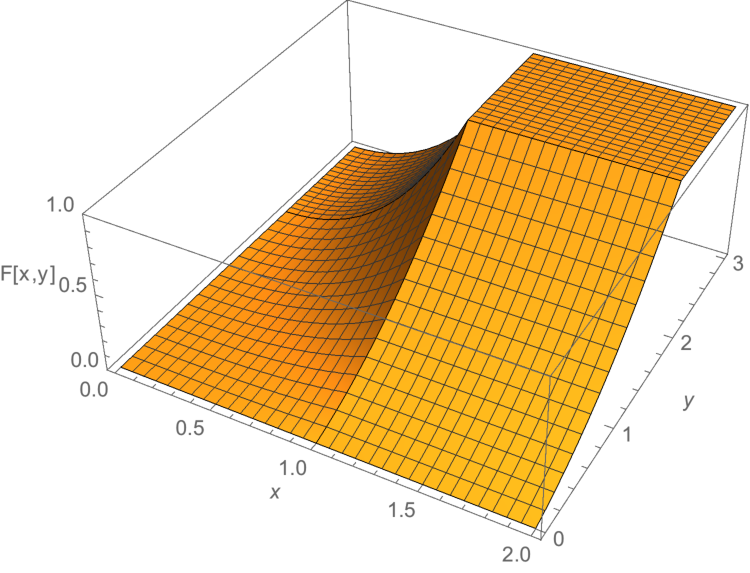
\includepdf[noautoscale=false]{images/cover.pdf}%
%% begin: half-title
\thispagestyle{empty}
{\titlepagefont\centering
\vspace*{0.28\textheight}
{\Huge Mathematical Statistics I}\\[2\baselineskip]
{\LARGE Based on course notes developed using Freund's Mathematical Statistics}\\
}
\clearpage
%% end:   half-title
%% begin: adcard
\thispagestyle{empty}
\null%
\clearpage
%% end:   adcard
%% begin: title page
%% Inspired by Peter Wilson's ``titleDB'' in ``titlepages'' CTAN package
\thispagestyle{empty}
{\titlepagefont\centering
\vspace*{0.14\textheight}
%% Target for xref to top-level element is ToC
\addtocontents{toc}{\protect\hypertarget{x:book:mathstat}{}}
{\Huge Mathematical Statistics I}\\[\baselineskip]
{\LARGE Based on course notes developed using Freund's Mathematical Statistics}\\[3\baselineskip]
{\Large Sean M. Laverty}\\[0.5\baselineskip]
{\Large University of Central Oklahoma}\\[3\baselineskip]
{\Large Mathematical Statistics I}\\[0.5\baselineskip]
{\Large March 24, 2021}\\}
\clearpage
%% end:   title page
%% begin: copyright-page
\thispagestyle{empty}
\hypertarget{x:colophon:front-colophon}{}\noindent
Sean M. Laverty is writing these notes to (hopefully) give us all a better chance at making it through the semester.%
\par
\vspace*{\stretch{2}}
\par\noindent
\textbf{Cover Design}:\ \ Sean M. Laverty
\par\vspace*{\stretch{2}}
\noindent{\bfseries Edition}: Emergency Edition 2021\par\medskip
\noindent{\bfseries Website}: \href{http:\slash{}\slash{}www.math.uco.edu}{\mono{www.math.uco.edu}}\par\medskip
\noindent\textcopyright{}2013\textendash{}2020\quad{}Sean M. Laverty\\[0.5\baselineskip]
Permission is granted to copy, distribute and\slash{}or modify this document under the terms of the GNU Free Documentation License, Version 1.2 or any later version published by the Free Software Foundation; with no Invariant Sections, no Front-Cover Texts, and no Back-Cover Texts.  A copy of the license is included in the appendix entitled ``GNU Free Documentation License.''  All trademarks\texttrademark{} are the registered\textregistered{} marks of their respective owners.\par\medskip
\vspace*{\stretch{1}}
\null\clearpage
%% end:   copyright-page
%% begin: dedication-page
\cleardoublepage
\thispagestyle{empty}
\vspace*{\stretch{1}}
\begin{center}\Large%
To students of mathematical and life sciences everywhere but specifically at UCO.%
\end{center}
\vspace*{\stretch{2}}
\clearpage
%% end:   dedication-page
%% begin: obverse-dedication-page (empty)
\thispagestyle{empty}
\null%
\clearpage
%% end:   obverse-dedication-page
%
%
\typeout{************************************************}
\typeout{Acknowledgements  Acknowledgements}
\typeout{************************************************}
%
\begin{acknowledgement}{Acknowledgements}{}{Acknowledgements}{}{}{x:acknowledgement:acknowledgement}
PreTexT group.%
\end{acknowledgement}
%
%
\typeout{************************************************}
\typeout{Preface  Preface}
\typeout{************************************************}
%
\begin{preface}{Preface}{}{Preface}{}{}{x:preface:preface}
See the \hyperlink{x:book:mathstat}{Table of Contents} for more.%
\nopagebreak\par%
\hfill\begin{tabular}[t]{l@{}}
Sean M. Laverty\\
Edmond, Oklahoma 2020
\end{tabular}\\\par
\end{preface}
%
%
\typeout{************************************************}
\typeout{Preface  Contributors to the 0\(^\mathrm{th}\) Edition}
\typeout{************************************************}
%
\begin{preface}{Contributors to the 0\(^\mathrm{th}\) Edition}{}{Contributors to the 0\(^\mathrm{th}\) Edition}{}{}{x:preface:contributors}
Many individuals have made this book possible.  We will try to thank a few of them here, and hope we have not forgotten anybody really important.%
\begin{multicols}{2}
\hypertarget{x:contributor:slaverty}{}%
\contributor{%
\contributorname{Sean M. Laverty}%
\contributorinfo{Department of Mathematics and Statistics\\
University of Central Oklahoma\\
Edmond, Oklahoma, USA\\
\mono{\href{mailto:slaverty@uco.edu}{\nolinkurl{slaverty@uco.edu}}}}%
}%
\end{multicols}
\end{preface}
%% begin: table of contents
%% Adjust Table of Contents
\setcounter{tocdepth}{1}
\renewcommand*\contentsname{Contents}
\tableofcontents
%% end:   table of contents
\mainmatter
%
%
\typeout{************************************************}
\typeout{Chapter 1 Counting}
\typeout{************************************************}
%
\begin{chapterptx}{Counting}{}{Counting}{}{}{x:chapter:chap-counting}
\begin{introduction}{}%
We will learn how to count.%
\end{introduction}%
%
%
\typeout{************************************************}
\typeout{Section 1.1 Counting}
\typeout{************************************************}
%
\begin{sectionptx}{Counting}{}{Counting}{}{}{x:section:section-counting}
\begin{introduction}{}%
Some words.%
\end{introduction}%
\begin{definition}{}{x:definition:counting}%
\(1, 2, 3, \dots\)%
\end{definition}
\end{sectionptx}
\end{chapterptx}
%
%
\typeout{************************************************}
\typeout{Chapter 2 Probability}
\typeout{************************************************}
%
\begin{chapterptx}{Probability}{}{Probability}{}{}{x:chapter:chap-prob}
\begin{introduction}{}%
We will learn about probability concepts.%
\end{introduction}%
%
%
\typeout{************************************************}
\typeout{Section 2.1 Probability}
\typeout{************************************************}
%
\begin{sectionptx}{Probability}{}{Probability}{}{}{x:section:section-probability}
\begin{introduction}{}%
Some words.%
\end{introduction}%
\begin{definition}{}{x:definition:probability}%
Sample text.%
\end{definition}
\end{sectionptx}
\end{chapterptx}
%
%
\typeout{************************************************}
\typeout{Chapter 3 Discrete Random Variables}
\typeout{************************************************}
%
\begin{chapterptx}{Discrete Random Variables}{}{Discrete Random Variables}{}{}{x:chapter:chap-discrete}
\begin{introduction}{}%
In this chapter we will step through using mathematical functions to describe probabilities associated with outcomes of experiments where the resulting measurements are discrete in nature.  We will essentially revisit all of the ideas from \hyperref[x:chapter:chap-prob]{Chapter~{\xreffont\ref{x:chapter:chap-prob}}}, but rely on the convenience of mathematical functions to replicate and advance our thinking and capabilities.%
\par
Given that, we will then start to make calculations about certain statistically and practically important properties of random variables using the concept of \emph{mathematical expectation}.  Following that, we will look at specific mathematical formulas for specific kinds of discrete random variables that describe common situations.%
\end{introduction}%
%
%
\typeout{************************************************}
\typeout{Section 3.1 Probability distributions}
\typeout{************************************************}
%
\begin{sectionptx}{Probability distributions}{}{Probability distributions}{}{}{x:section:section-probability-distributions}
\begin{introduction}{}%
Some words.%
\end{introduction}%
%
%
\typeout{************************************************}
\typeout{Subsection 3.1.1 Random variables and probability distributions}
\typeout{************************************************}
%
\begin{subsectionptx}{Random variables and probability distributions}{}{Random variables and probability distributions}{}{}{x:subsection:sub-single-variable-disc}
\begin{introduction}{}%
See sections 3.1, 3.2. Recommended problems: (pg80)1,3,4ab,5,6,7a%
\end{introduction}%
\begin{definition}{probability distribution.}{x:definition:def-probability-distribution-3-2}%
If \(\displaystyle X\) is a discrete random variable, the function given by \(\displaystyle f(x) = P(X = x)\) for each \(\displaystyle
x\) within the range of \(\displaystyle X\) is called the \terminology{probability distribution}.%
\end{definition}
\begin{theorem}{conditions for probability distribution.}{}{x:theorem:thm-conditions-3-1}%
A function can serve as the probability distribution for a discrete random variable \(\displaystyle X\) if and only if its values, \(\displaystyle f(x)\), satisfy the conditions%
\begin{enumerate}
\item{}\(\displaystyle f(x) \ge 0\) for each value within its domain;%
\item{}\(\displaystyle \sum_x f(x) = 1\), where the summation extends over all the values within its domain%
\end{enumerate}
%
\end{theorem}
\begin{definition}{distribution function.}{x:definition:def-distribution-function-3-3}%
If \(\displaystyle X\) is a discrete random variable, the function given by  where \(\displaystyle f(t)\) is the value of the probability distribution of \(\displaystyle X\) at \(\displaystyle t\), is called the \terminology{distribution function}, or the \terminology{cumulative distribution (function)}, of \(\displaystyle X\).%
\end{definition}
\begin{theorem}{properties of a distribution function.}{}{x:theorem:thm-3-2}%
The values \(\displaystyle F(x)\) of the distribution function of a discrete random variable \(\displaystyle X\) satisfy the conditions%
\begin{enumerate}
\item{}\(\displaystyle F(-\infty) = 0\) and \(\displaystyle F(\infty)
= 1\) (more carefully stated as \(\displaystyle
\lim_{x\to-\infty}F(x) = 0\) and \(\displaystyle \lim_{x\to\infty}
F(x) = 1\));%
\item{}if \(\displaystyle a \lt b\), then \(\displaystyle F(a) \le
F(b)\) for any real numbers \(\displaystyle a\) and \(\displaystyle b\)%
\end{enumerate}
%
\end{theorem}
\begin{example}{Verifying a simple probability mass function.}{x:example:ex-disc-pmf}%
Identify whether the function \(f(x) = \dfrac{2x-1}{5}\) is a probability mass function for the discrete random variable \(X\) with values \(x=1,2,3,4,5\).  If it is not a valid distribution ``fix it''.%
\par\smallskip%
\noindent\textbf{\blocktitlefont Solution}.\hypertarget{g:solution:idp140361417157328}{}\quad{}Notice that values of \(f(x) \ge 0\) for all possible \(x\), but%
\begin{equation*}
\sum\limits_{x=1}^5 f(x) = 5 \neq 1.
\end{equation*}
\begin{tableptx}{\textbf{}}{g:table:idp140361416993488}{}%
\centering
{\tabularfont%
\begin{tabular}{ll}
\multicolumn{1}{c}{\(x\)}&\multicolumn{1}{c}{\(f(x)\)}\tabularnewline\hrulemedium
1&\(f(1) = \frac{1}{5}\)\tabularnewline[0pt]
2&\(f(2) = \frac{3}{5}\)\tabularnewline[0pt]
3&\(f(3) = \frac{5}{5}\)\tabularnewline[0pt]
4&\(f(4) = \frac{7}{5}\)\tabularnewline[0pt]
5&\(f(5) = \frac{9}{5}\)
\end{tabular}
}%
\end{tableptx}%
 The function must be rescaled so that probabilities sum to one.  The function \(f(x) =
\dfrac{2x-1}{25}\) is a valid probability mass function for the values of the random variable mentioned above. \begin{tableptx}{\textbf{}}{g:table:idp140361416816208}{}%
\centering
{\tabularfont%
\begin{tabular}{ll}
\multicolumn{1}{c}{\(x\)}&\multicolumn{1}{c}{\(f(x) = \dfrac{2x-1}{25}\)}\tabularnewline\hrulemedium
1&\(f(1) = \frac{1}{25}\)\tabularnewline[0pt]
2&\(f(2) = \frac{3}{25}\)\tabularnewline[0pt]
3&\(f(3) = \frac{5}{25}\)\tabularnewline[0pt]
4&\(f(4) = \frac{7}{25}\)\tabularnewline[0pt]
5&\(f(5) = \frac{9}{25}\)
\end{tabular}
}%
\end{tableptx}%
%
\end{example}
\begin{example}{CDF of a simple probability mass function.}{x:example:ex-disc-pmf-to-cdf}%
The function \(f(x) = \dfrac{2x-1}{25}\) is a probability mass function for the discrete random variable \(X\) with values \(x=1,2,3,4,5\).  Find the cumulative distribution function.%
\par\smallskip%
\noindent\textbf{\blocktitlefont Solution}.\hypertarget{g:solution:idp140361417107632}{}\quad{}\begin{tableptx}{\textbf{}}{g:table:idp140361416974432}{}%
\centering
{\tabularfont%
\begin{tabular}{lll}
\multicolumn{1}{c}{\(x\)}&\multicolumn{1}{c}{\(\operatorname{Pr}(X \le x)\)}&\multicolumn{1}{c}{\(F(x)\)}\tabularnewline\hrulemedium
1&\(f(1) \)&\(\frac{1}{25}\)\tabularnewline[0pt]
2&\(f(1) + f(2) \)&\(\frac{1}{25} + \frac{3}{25}\)\tabularnewline[0pt]
3&\(f(1) + f(2) + f(3) \)&\(\frac{4}{25} + \frac{5}{25}\)\tabularnewline[0pt]
4&\(f(1) + f(2) + f(3) + f(4) \)&\(\frac{9}{25} + \frac{7}{25}\)\tabularnewline[0pt]
5&\(f(1) + f(2) + f(3) + f(4) + f(5) \)&\(\frac{16}{25} + \frac{9}{25}\)
\end{tabular}
}%
\end{tableptx}%
 We have%
\begin{equation*}
F(x) = \begin{cases} 0, \amp \quad x \lt 1\\
\frac{1}{25}, \amp \quad 1 \le x \lt 2\\
\frac{4}{25}, \amp \quad 2 \le x \lt 3\\
\frac{9}{25}, \amp \quad 3 \le x \lt 4\\
\frac{16}{25}, \amp \quad 4 \le x \lt 5\\
1, \amp \quad 5 \le x
\end{cases}
\end{equation*}
The function \(F(x)\), is piecewise constant, accumulating new probability at the values of \(x = 1, 2, 3, 4, 5\).%
\end{example}
\end{subsectionptx}
%
%
\typeout{************************************************}
\typeout{Exercises 3.1.2 Exercises}
\typeout{************************************************}
%
\begin{exercises-subsection}{Exercises}{}{Exercises}{}{}{g:exercises:idp140361416979584}
\begin{divisionexercise}{1}{Problem 3.1.}{}{g:exercise:idp140361416979808}%
For each of the following, determine whether the given values can serve as the values of a probability distribution of a random variable with the range \(x = 1, 2, 3, \text{and } 4\):%
\begin{enumerate}[label=(\alph*)]
\item{}\(\displaystyle f(1) = 0.25,f(2) = 0.75,f(3) = 0.25, \text{and } f(4) =
0.25\)%
; \item{}\(\displaystyle f(1) = 0.15,f(2) = 0.27,f(3) = 0.29, \text{and } f(4) =
0.29\)%
; \item{}\(\displaystyle f(1) = \dfrac{1}{19},f(2) = \dfrac{10}{19},f(3) =
\dfrac{2}{19}, \text{and } f(4) = \dfrac{5}{19}\)%
.\end{enumerate}
%
\end{divisionexercise}%
\begin{divisionexercise}{2}{Problem 3.3.}{}{g:exercise:idp140361416918432}%
Verify that \(\displaystyle f(x) = \dfrac{2x}{k(k+1)}\) for \(x=1, 2,
3, \dots, k\) can serve as the probability distribution of a random variable with the given range. \emph{Bonus:} Find or describe \(F(x)\).\textbraceright{}%
\end{divisionexercise}%
\begin{divisionexercise}{3}{Problem 3.4b.}{}{g:exercise:idp140361416957328}%
Determine \(c\) so that the function \(\displaystyle f(x) =
c{5\choose x}\) for \(x = 0, 1, 2, 3, 4, 5\) can serve as a probability distribution of a random variable with the given range.%
\end{divisionexercise}%
\begin{divisionexercise}{4}{Problem 3.5.}{}{g:exercise:idp140361455125536}%
For what values of \(k\) an%
\begin{equation*}
f(x) = (1-k)k^x
\end{equation*}
serve as the values of the probability distribution of a random variable with countably infinite range \(x = 0, 1, 2, \dots\)?%
\end{divisionexercise}%
\begin{divisionexercise}{5}{Problem 3.7a.}{}{g:exercise:idp140361455126832}%
Show that there are no values of \(c\) such that%
\begin{equation*}
f(x) =
\dfrac{c}{x}
\end{equation*}
can serve as the values of the probability distribution of a random variable with countably infinite range \(x = 0, 1, 2, \dots\)%
\end{divisionexercise}%
\begin{divisionexercise}{6}{Problem 3.6.}{}{g:exercise:idp140361455131632}%
Construct a probability histogram for the probability distribution%
\begin{equation*}
f(x) = \dfrac{{2\choose x}{4\choose{3-x}}}{{6\choose3}} \text{ for
}x=0, 1, 2
\end{equation*}
%
\end{divisionexercise}%
\begin{divisionexercise}{7}{Problem 3.87.}{}{g:exercise:idp140361455132944}%
The probability distribution of \(V\), the number of weekly accidents at a certain intersection, is given by \(g(0) = 0.4, g(1) =
0.3, g(2) = 0.2, g(3) = 0.1\). Construct the distribution function of \(V\) and draw its graph.%
\end{divisionexercise}%
\begin{divisionexercise}{8}{Problem 3.88.}{}{g:exercise:idp140361455135024}%
Using the statement and result of the previous problem, find the probability that there will be at least two accidents in any one week using%
\begin{enumerate}[label=(\alph*)]
\item{}the original probabilities, and%
\item{}the values of the distribution function.%
\end{enumerate}
%
\end{divisionexercise}%
\end{exercises-subsection}
\end{sectionptx}
%
%
\typeout{************************************************}
\typeout{Section 3.2 Mathematical expectation of discrete random variables}
\typeout{************************************************}
%
\begin{sectionptx}{Mathematical expectation of discrete random variables}{}{Mathematical expectation of discrete random variables}{}{}{x:section:section-discrete-expectation}
\begin{introduction}{}%
This is the start of Chapter 4 in Freund's Mathematical Statistics. In the first pass we will study the major topics of this chapter with a focus on those applying to discrete random variables.%
\end{introduction}%
%
%
\typeout{************************************************}
\typeout{Subsection 3.2.1 Expected value}
\typeout{************************************************}
%
\begin{subsectionptx}{Expected value}{}{Expected value}{}{}{x:subsection:sub-expectation}
See section 4.1 - 4.2. Recommended problems: (pg 136) 7, 9, 10, 11, (pg 161) 60%
\begin{definition}{expected value.}{x:definition:def-expected-value-4-1}%
If \(X\) is a discrete random variable and \(\displaystyle f(x)\) is the value of its probability distribution at \(X\), the \terminology{expected value} of \(X\) is given by%
\begin{equation*}
E[X] = \sum_x x\cdot f(x)
\end{equation*}
%
\end{definition}
\begin{example}{expected value of a random variable.}{x:example:ex-disc-pmf-mean}%
Recall the function \(f(x) = \dfrac{2x-1}{25}\) from \hyperref[x:example:ex-disc-pmf]{Example~{\xreffont\ref{x:example:ex-disc-pmf}}}, which is a probability mass function for the discrete random variable \(X\) with values \(x=1,2,3,4,5\).  Find \(\mu = E[X]\)%
\par\smallskip%
\noindent\textbf{\blocktitlefont Solution}.\hypertarget{g:solution:idp140361455144304}{}\quad{}Since \(\mu = E[X]\), we have%
\begin{align*}
\mu = E[X] \amp = \sum\limits_{x=1}^5 x\cdot f(x)\\
\amp = \sum\limits_{x=1}^5 x\cdot \left(\dfrac{2x-1}{25}\right)\\
\amp = \sum\limits_{x=1}^5 \left(\dfrac{2}{25}x^2 - \dfrac{1}{25}x\right)\\
\amp = \left(\dfrac{2}{25}\sum\limits_{x=1}^5 x^2\right) - \left(\dfrac{1}{25}\sum\limits_{x=1}^5 x\right)\\
\amp = \left(\dfrac{2}{25}\left(55\right)\right) - \left(\dfrac{1}{25}\left(15\right)\right)\\
\mu = E[X] \amp = \dfrac{19}{5}
\end{align*}
%
\par
So, the mean of the distribution of the random variable \(X\) is%
\begin{equation*}
\mu = E[X] = \dfrac{19}{6}\text{.}
\end{equation*}
%
\end{example}
\begin{theorem}{expected value of a function of a random variable.}{}{x:theorem:thm-expected-value-function-random-variable-4-1}%
If \(X\) is a discrete random variable and \(\displaystyle f(x)\) is the value of its probability distribution at \(X\), the expected value of \(\displaystyle
g(X)\) is given by%
\begin{equation*}
E[g(X)] = \sum_x g(x)\cdot f(x)
\end{equation*}
%
\end{theorem}
\begin{theorem}{expectation of a linear function.}{}{x:theorem:thm-4-2}%
If \(\displaystyle a\) and \(\displaystyle b\) are constants, then \(\displaystyle E[aX +b] = aE[X]+b\).%
\end{theorem}
\begin{corollary}{}{}{x:corollary:cor-4-1}%
If a is a constant, then \(\displaystyle E[aX] = aE[X]\).%
\end{corollary}
\begin{corollary}{}{}{x:corollary:cor-4-2}%
If b is a constant, then \(\displaystyle E[b] = b\).%
\end{corollary}
\end{subsectionptx}
%
%
\typeout{************************************************}
\typeout{Exercises 3.2.2 Exercises}
\typeout{************************************************}
%
\begin{exercises-subsection}{Exercises}{}{Exercises}{}{}{g:exercises:idp140361455158144}
\begin{divisionexercise}{1}{Problem 4.9.}{}{g:exercise:idp140361455158368}%
Suppose that \(X\) takes on values \(0, 1, 2, 3\) with probabilities \(\dfrac{1}{125}, \dfrac{12}{125}, \dfrac{48}{125},
\dfrac{64}{125}\)%
\begin{enumerate}[label=(\alph*)]
\item{}Find \(E[X]\) and \(E[X^2]\)%
\item{}Determine the value of \(E[(3X + 2)^2]\)%
\end{enumerate}
%
\end{divisionexercise}%
\end{exercises-subsection}
%
%
\typeout{************************************************}
\typeout{Subsection 3.2.3 Expected value}
\typeout{************************************************}
%
\begin{subsectionptx}{Expected value}{}{Expected value}{}{}{x:subsection:sub-moments}
See section 4.3. Recommended problems: 4.3 (pg 146) 20, 22, 23, 31, 33, 34, 40, (pg 162) 69, 73, 75%
\begin{definition}{moments about the origin.}{x:definition:def-moments-about-origin-4-2}%
The \(\displaystyle r^\text{th}\) \terminology{moment about the origin} of a random variable \(X\), denoted by \(\displaystyle \mu_r'\), is the expected value of \(\displaystyle
(X)^r\); symbolically%
\begin{equation*}
\mu_r'=E[(X)^r] = \sum_x x^r\cdot f(x)
\end{equation*}
for \(\displaystyle r =
0,1,2, \dots\) when \(X\) is discrete.%
\end{definition}
\begin{definition}{mean of a discrete random variable.}{x:definition:def-mean-4-3}%
\(\displaystyle \mu_1'\) is called the \terminology{mean} of the distribution of \(X\), or simply the \terminology{mean} of \(X\); and it is denoted by \(\displaystyle
\mu\).\end{definition}
\begin{definition}{moments about the mean.}{x:definition:def-moments-about-mean-4-4}%
The \(\displaystyle r^\text{th}\) \terminology{moment about the mean} of a random variable \(X\), denoted by \(\displaystyle \mu_r\), is the expected value of \(\displaystyle
(X-\mu)^r\); symbolically%
\begin{equation*}
\mu_r=E[(X-\mu)^r] = \sum_x (x-\mu)^r\cdot f(x)
\end{equation*}
for \(\displaystyle r =
0,1,2, \dots\) when \(X\) is discrete.%
\end{definition}
\begin{example}{variance of a random variable.}{x:example:ex-disc-pmf-variance}%
Recall the function \(f(x) = \dfrac{2x-1}{25}\) from \hyperref[x:example:ex-disc-pmf]{Example~{\xreffont\ref{x:example:ex-disc-pmf}}} and \hyperref[x:example:ex-disc-pmf-mean]{Example~{\xreffont\ref{x:example:ex-disc-pmf-mean}}}, which is a probability mass function for the discrete random variable \(X\) with values \(x=1,2,3,4,5\).  Find \(\sigma^2 = \mu_{2} = E[(X - \mu)^2]\)%
\par\smallskip%
\noindent\textbf{\blocktitlefont Solution}.\hypertarget{g:solution:idp140361455176096}{}\quad{}Recall that \(\sigma^2 = \mu_{2}' - \left(E[x]\right)^2\) or \(\sigma^2 = E[X^2] - \left(E[x]\right)^2\). Since \(\mu_{2}' = E[X^2]\), we have%
\begin{align*}
\mu_{2}' = E[X^2] \amp = \sum\limits_{x=1}^5 x^2\cdot f(x)\\
\amp = \sum\limits_{x=1}^5 x^2\cdot \left(\dfrac{2x-1}{25}\right)\\
\amp = \sum\limits_{x=1}^5 \left(\dfrac{2}{25}x^3 - \dfrac{1}{25}x^2\right)\\
\amp = \left(\dfrac{2}{25}\sum\limits_{x=1}^5 x^3\right) - \left(\dfrac{1}{25}\sum\limits_{x=1}^5 x^2\right)\\
\amp = \left(\dfrac{2}{25}\left(225\right)\right) - \left(\dfrac{1}{25}\left(55\right)\right)\\
\mu_{2}' = E[X^2] \amp = \dfrac{79}{25}
\end{align*}
%
\par
Now, by theorem,%
\begin{align*}
\sigma^2 = \amp E[X^2] - \left(E[x]\right)^2\\
= \amp \dfrac{79}{5} - \left(\dfrac{19}{5}\right)^2\\
\sigma^2 = \amp  \dfrac{34}{25}
\end{align*}
%
\end{example}
Now, you could imagine in some cases the moments being difficult to calculate as sums. We sometimes take the approach of building what are called moment-generating functions. These are mathematical functions whose purpose is to generate the moments of a distribution that we might need.%
\end{subsectionptx}
%
%
\typeout{************************************************}
\typeout{Exercises 3.2.4 Exercises}
\typeout{************************************************}
%
\begin{exercises-subsection}{Exercises}{}{Exercises}{}{}{g:exercises:idp140361455184272}
\begin{divisionexercise}{1}{Problem 4.18.}{}{g:exercise:idp140361455184400}%
Find \(\mu\), \(\mu_2'\), and \(\sigma^2\) for the random variable \(X\) that has probability distribution \(f(x) = 0.5 \text{
for } x= \pm 2\).%
\end{divisionexercise}%
\end{exercises-subsection}
%
%
\typeout{************************************************}
\typeout{Subsection 3.2.5 Moment-generating functions}
\typeout{************************************************}
%
\begin{subsectionptx}{Moment-generating functions}{}{Moment-generating functions}{}{}{x:subsection:sub-mgf}
See section 4.5.%
\begin{definition}{moment-generating function.}{x:definition:def-mgf-4-6}%
The \terminology{moment-generating function} of a random variable \(X\), where it exists, is given by%
\begin{equation*}
\displaystyle
M_X(t) = E[e^{tX}] = \sum_x e^{tx}\cdot f(x)
\end{equation*}
when \(X\) is discrete.%
\end{definition}
Notce that a moment-generating function \(\displaystyle M_X(t)\) itself is a function of the variable \(\displaystyle t\) not \(X\). As it turns out, we are most interested in values of the function at or near \(\displaystyle t=0\).%
\begin{example}{moment-generating function via Taylor series.}{x:example:ex-maclaurin}%
Recall that the Maclaurin series (Taylor series around zero) for \(\displaystyle e^{tx}\) is%
\begin{equation*}
e^{tx} = 1 + tx +
\frac{1}{2!}\left(tx\right)^2 + \frac{1}{3!}\left(tx\right)^3 + \cdots +
\frac{1}{r!}\left(tx\right)^r + \cdots
\end{equation*}
This means (in the discrete case), that%
\begin{equation*}
\begin{aligned}[t]
M_X(t) \amp = \sum_x e^{tx} f(x)\\
\amp = \sum_x \left(1 + tx + \frac{1}{2!}(tx)^2 +
\frac{1}{3!}\left(tx\right)^3 + \cdots + \frac{1}{r!}\left(tx\right)^r +
\cdots\right) f(x)\\
\amp = \sum_x (f(x) + txf(x) + \frac{t^2}{2!}x^2f(x) +
\frac{t^3}{3!}x^3f(x) + \cdots + \frac{t^r}{r!}x^rf(x) + \cdots)\\
\amp = \sum_xf(x) + t\sum_x xf(x) + \frac{t^2}{2!}\sum_x x^2f(x) +
\frac{t^3}{3!}\sum_x x^3f(x) + \cdots + \frac{t^r}{r!}\sum_x x^rf(x) +
\cdots
\end{aligned}
\end{equation*}
Looking closely, at%
\begin{equation*}
M_X(t) = \sum_xf(x) + \left(\sum_x xf(x)\right)t
+ \left(\sum_x x^2f(x)\right)\frac{t^2}{2!} + \left(\sum_x
x^3f(x)\right)\frac{t^3}{3!} + \cdots + \left(\sum_x
x^rf(x)\right)\frac{t^r}{r!} + \cdots
\end{equation*}
coefficients of the terms \(\displaystyle \dfrac{t^r}{r!}\) are the moments about the origin \(\displaystyle \mu_r' = \sum_x x^r f(x)\)%
\end{example}
\begin{example}{moment-generating function for three coins.}{x:example:ex-three-coins-mgf}%
Recall the probability distribution \(f(x) = P(X = x) =
\dfrac{{3\choose x}}{8} \text{ for } x = 0, 1, 2, 3\) (this was used earlier to determine the probabilities of \(x\) heads on three flips of a coin).%
\begin{equation*}
\begin{aligned}[t]
M_X(t) \amp = \sum_x e^{tx} f(x)\\
\amp = 1 \cdot \frac{1}{8} + e^{t} \cdot \frac{3}{8}+ e^{2t} \cdot
\frac{3}{8} + e^{3t} \cdot \frac{1}{8}\\
\amp = \frac{1}{8} \left(1 + 3e^{t} + 3e^{2t} + e^{3t}\right)\\
M_X(t) \amp = \frac{1}{8} (1+e^t)^3\\
\end{aligned}
\end{equation*}
%
\end{example}
\begin{theorem}{moments via differentiation.}{}{x:theorem:thm-4-9}%
The \(r^\text{th}\) moment about the origin, \(\mu_r'\), can be written%
\begin{equation*}
\displaystyle \mu_r' = \dfrac{d^rM_X(t)}{dt^r}\Big|_{t=0}
\end{equation*}
%
\end{theorem}
\begin{example}{moment-generating function for three cards, via differentiation.}{x:example:ex-three-coins-mgf2}%
Referencing \hyperref[x:example:ex-three-coins-mgf]{Example~{\xreffont\ref{x:example:ex-three-coins-mgf}}}, the mean of the random variable, given by \(\mu_1'\), whose MGF is \(M_X(t) =
\frac{1}{8} (1+e^t)^3\) is found as follows%
\begin{equation*}
\begin{aligned}[t]
\mu_1' \amp = \left(\dfrac{d}{dt}\left(\frac{1}{8}
(1+e^t)^3\right)\right)\Big|_{t=0}\\
\amp = \left(\frac{3}{8} (1+e^t)^2e^t\right)\Big|_{t=0}\\
\amp = \left(\frac{3}{8} (2)^2\right)\\
\mu_1' \amp = \frac{3}{2}
\end{aligned}
\end{equation*}
%
\end{example}
So, \emph{given} a moment-generating function, a relatively simple application of calculus allows us to replace a more tedious calculation of the moment from its definition.%
\begin{theorem}{moment-generating function of functions of a random variable.}{}{x:theorem:thm-4-10}%
If \(\displaystyle a\) and \(\displaystyle b\) are constants, then%
\begin{enumerate}
\item{}\(\displaystyle M_{X+a}(t) = E[e^{(X+a)t}] = e^{at} \cdot
M_X(t)\);%
\item{}\(\displaystyle M_{bX}(t) = E[e^{bXt}] = M_X(bt)\);%
\item{}\(\displaystyle M_{\frac{X+a}{b}}(t) =
E\left[e^{\left(\frac{X+a}{b}\right)t}\right] = e^{(a/b)t} \cdot
M_X\left(\frac{t}{b}\right)\);%
\end{enumerate}
%
\end{theorem}
The rules in \hyperref[x:theorem:thm-4-10]{Theorem~{\xreffont\ref{x:theorem:thm-4-10}}} allow us to calculate moment-generating functions of simple functions of a random variable.%
\end{subsectionptx}
%
%
\typeout{************************************************}
\typeout{Exercises 3.2.6 Exercises}
\typeout{************************************************}
%
\begin{exercises-subsection}{Exercises}{}{Exercises}{}{}{g:exercises:idp140361455187632}
\begin{divisionexercise}{1}{Problem 4.33.}{}{g:exercise:idp140361455210144}%
Find the moment-generating function of the discrete random variable \(X\) that has the probability distribution%
\begin{equation*}
f(x) =
2\left(\dfrac{1}{3}\right)^x \text{ for } x = 1, 2, 3, \dots
\end{equation*}
and use it to determine the values of \(\mu_1'\) and \(\mu_2'\).%
\end{divisionexercise}%
\begin{divisionexercise}{2}{Problem 4.40.}{}{g:exercise:idp140361455212688}%
Given the moment-generating function \(X_X(t) = e^{3t+8t^2}\), find the moment generating function of the random variable \(Z =
\dfrac{1}{4}\left(X-3\right)\) and use it to determine the mean and variance of \(Z\).%
\end{divisionexercise}%
\end{exercises-subsection}
\end{sectionptx}
%
%
\typeout{************************************************}
\typeout{Section 3.3 Special probability distributions}
\typeout{************************************************}
%
\begin{sectionptx}{Special probability distributions}{}{Special probability distributions}{}{}{x:section:section-special-distributions}
\begin{introduction}{}%
Now we look at a collection of formulas for probability distributions. These describe how probabilities are assigned across a range of discrete values of a random variable. It turns out to be the case that values of random variables associated with certain kinds of experiments follow certain formulas. In this chapter, we will look at the formulas that describe certain discrete random variables.%
\par
For the purposes of generality we will emphasize that certain formulas include one or more parameters, these are symbols to which we will associate particular numerical values, much like we do \(m\) and \(b\) in the formula \(y = f(x) = mx+b\). We should have a general understanding of something that follows this relationship and an understanding of the roles of both \(m\) and \(b\) in specifying that relationship.%
\end{introduction}%
%
%
\typeout{************************************************}
\typeout{Subsection 3.3.1 Discrete uniform}
\typeout{************************************************}
%
\begin{subsectionptx}{Discrete uniform}{}{Discrete uniform}{}{}{x:subsection:sub-discrete-unif}
\begin{definition}{discrete uniform distribution.}{x:definition:def-discrete-unif}%
A discrete random variable \(\displaystyle X\) has a \terminology{discrete uniform distribution} and is referred to as a \terminology{discrete uniform random variable} if and only if its probability distribution is given by%
\begin{equation*}
f(x) = \frac{1}{k} \text{ for }
x = x_1, x_2, \dots, x_k \text{ where }x_i\ne x_j \text{ for } i \ne
j\text{.}
\end{equation*}
%
\end{definition}
This is sometimes written as \(\operatorname{DU}(k)\), where \(k\) is the parameter of the distribution.%
\begin{example}{mean of a discrete uniform distribution.}{x:example:ex-disc-unif-mean}%
Find the mean of a discrete uniform random variable (or of the discrete uniform distribution).%
\textbf{\blocktitlefont Solution}.\quad{}Recall that%
\begin{equation*}
f(x) = \frac{1}{k} \text{ for } x = x_1, x_2, \dots,
x_k \text{ where }x_i\ne x_j \text{ for } i \ne j
\end{equation*}
and that%
\begin{equation*}
\mu
= \sum_x x\cdot f(x)\text{.}
\end{equation*}
This becomes%
\begin{equation*}
\mu = \sum_{i=1}^k
x_i\left(\frac{1}{k}\right)\text{.}
\end{equation*}
This is about as far as we can go in general without knowing more about \(k\) or the values of \(x_i\).%
\end{example}
Similar to the previous ``Example'', the variance of a discrete uniform random variable (or of the discrete uniform distribution) is given by%
\begin{equation*}
\sigma^2 = \sum_x (x-\mu)^2\cdot f(x)= \sum_x (x-\mu)^2
\left(\frac{1}{k}\right)\text{.}
\end{equation*}
Once again, this is about as far as we can go in general.%
\begin{example}{simple discrete uniform distribution.}{x:example:ex-disc-unif-simple}%
Find the mean of a discrete uniform random variable (or of the discrete uniform distribution) for which \(x_i = i\).%
\textbf{\blocktitlefont Solution}.\quad{}Recall that%
\begin{equation*}
f(x) = \frac{1}{k} \text{ for } x = 1, 2, \dots,
k
\end{equation*}
and that%
\begin{equation*}
\mu = \sum_x x\cdot f(x)\text{.}
\end{equation*}
This becomes%
\begin{equation*}
\begin{aligned}[t]
\mu \amp = \sum_{i=1}^k i\left(\frac{1}{k}\right)\\
\amp = \frac{1}{k}\left(\sum_{i=1}^k i\right)\\
\amp = \frac{1}{k}\left(\dfrac{k(k+1)}{2}\right)\\
\mu	\amp = \dfrac{k+1}{2}
\end{aligned}\text{.}
\end{equation*}
Now, verify our earlier work on the mean number of dots to show on a balanced, 6-sided die.%
\end{example}
\end{subsectionptx}
%
%
\typeout{************************************************}
\typeout{Exercises 3.3.2 Exercises}
\typeout{************************************************}
%
\begin{exercises-subsection}{Exercises}{}{Exercises}{}{}{g:exercises:idp140361455232544}
\begin{divisionexercise}{1}{5.2.}{}{g:exercise:idp140361455232768}%
If \(X\) has a discrete uniform distribution \(f(x) =
\dfrac{1}{k}\) for \(x = 1, 2, \dots, k\), show that its moment-generating function is given by%
\begin{equation*}
M_x(t) =
\dfrac{e^t(1-e^{kt})}{k(1-e^t)}\text{.}
\end{equation*}
%
\end{divisionexercise}%
\end{exercises-subsection}
%
%
\typeout{************************************************}
\typeout{Subsection 3.3.3 Bernoulli and Binomial distributions}
\typeout{************************************************}
%
\begin{subsectionptx}{Bernoulli and Binomial distributions}{}{Bernoulli and Binomial distributions}{}{}{x:subsection:sub-discrete-bern-bin}
\begin{introduction}{}%
Consider an experiment with two possible outcomes, flipping a coin for example. We consider one of those outcomes, say 'heads' as a success, and the other of those outcomes, in this case 'tails\textasciigrave{} as a failure. We allow these outcomes to each occur with a given probability. Here \(\theta\) gives the probability of 'success' and \(1-\theta\) is the corresponding probability of 'failure'.%
\par
Though the outcome of a single event may be useful, the Bernoulli distribution is perhaps most useful as a building block to describe the results of more complex experiments.%
\par
You will find tools for visualization at the following \href{https://buddy.uco.edu/shiny/slaverty/mathstat/Binomial/}{link}.%
\end{introduction}%
\begin{definition}{Bernoulli distribution.}{x:definition:def-bern}%
A discrete random variable \(\displaystyle X\) has a \terminology{Bernoulli distribution} and is referred to as a \terminology{Bernoulli random variable} if and only if its probability distribution is given by%
\begin{equation*}
f(x; \theta) = \theta^x(1-\theta)^{1-x}
\text{ for }x = 0, 1\text{.}
\end{equation*}
%
\end{definition}
\begin{example}{mean and variance of a Bernoulli distribution.}{x:example:ex-bern-mean-var}%
Find the mean and variance of a Bernoulli random variable (or of the Bernoulli distribution).%
\textbf{\blocktitlefont Solution}.\quad{}Generally we calculate the mean as%
\begin{equation*}
\mu = \sum_x x\cdot f(x)\text{.}
\end{equation*}
Specifically this becomes%
\begin{equation*}
\begin{aligned}[t]
\mu \amp = \sum_{i=0}^1 x f(x; \theta)\\
\amp = 0\left(\theta^0(1-\theta)^1\right) +
1\left(\theta^1(1-\theta)^0\right)\\
\mu \amp = \theta
\end{aligned}\text{.}
\end{equation*}
%
\par
We calculate the variance as \(\sigma^2 =
E[X^2]-\left(E[X]\right)^2\). Keep in mind that we now know that \(E[X] = \theta\), so we know that \(\left(E[X]\right)^2 =
\theta^2\)%
\par
Now%
\begin{equation*}
\begin{aligned}[t]
E[X^2] \amp = \sum_{i=0}^1 x^2 f(x; \theta)\\
\amp = 0^2\left(\theta^0(1-\theta)^1\right) +
1^2\left(\theta^1(1-\theta)^0\right)\\
E[X^2] \amp = \theta
\end{aligned}
\end{equation*}
Given this,%
\begin{equation*}
\begin{aligned}[t]
\sigma^2 \amp = E[X^2]-\left(E[X]\right)^2\\
\amp = \theta - \theta^2 \\
\sigma^2 \amp = \theta(1-\theta)
\end{aligned}
\end{equation*}
%
\end{example}
\begin{example}{moment-generating function of a Bernoulli distribution.}{x:example:ex-bern-mgf}%
Find the moment-generating function of a Bernoulli random variable (or of the Bernoulli distribution).%
\textbf{\blocktitlefont Solution}.\quad{}Recall that \(\displaystyle M_X(t) = E[e^{tx}] = \sum_x e^{tx} f(x;
\theta)\). This becomes%
\begin{equation*}
\begin{aligned}[t]
M_X(t) \amp = \sum_{x=0}^1 e^{tx} f(x; \theta)\\
\amp = e^{0\cdot t}\left(\theta^0(1-\theta)^1\right) + e^{1\cdot
t}\left(\theta^1(1-\theta)^0\right)\\
\amp = (1-\theta) + \theta e^t\\
M_X(t) \amp = 1 + \theta (e^t-1)
\end{aligned}\text{.}
\end{equation*}
%
\end{example}
You could use the moment-generating function and the earlier theorem to calculate moments about the origin used to find the mean and variance.%
\par
Consider now a new random variable \(Y\) whose value is the sum of independent Bernoulli trials. This new variable has a 'binomial distribution' as defined below.%
\begin{definition}{binomial distribution.}{x:definition:def-bin}%
A discrete random variable \(\displaystyle X\) has a \terminology{binomial distribution} and is referred to as a \terminology{binomial random variable} if and only if its probability distribution is given by%
\begin{equation*}
b(x; n, \theta) = {n\choose
x}\theta^x(1-\theta)^{n-x} \text{ for }x = 0, 1, \dots, n\text{.}
\end{equation*}
%
\end{definition}
In the definition, the term \(\displaystyle {n \choose x}\) gives the number of ways to select the order of the \(x\) successes in \(n\) trials. The values of \(b(x; n, \theta)\) give the terms in the expansion of \(\displaystyle
\left((1-\theta) + \theta\right)^n\) (for more see \hyperref[x:remark:rmk-connection-to-pascal]{Remark~{\xreffont\ref{x:remark:rmk-connection-to-pascal}}}).%
\begin{remark}{Connection to binomial theorem.}{x:remark:rmk-connection-to-pascal}%
You may be wondering, what does \(\displaystyle
\left((1-\theta) + \theta\right)^n\) have to do with anything?%
\par
Recall that the binomial theorem suggests that%
\begin{equation*}
(a+b)^{n} = \sum\limits_{x=0}^n {n \choose x}a^{n-x}b^x = {n \choose 0} a^{n}b^{0} + {n \choose 1} a^{n-1}b^{1} + \dots + {n \choose n} a^{0}b^{n}.
\end{equation*}
By connecting these, we see that with \(b = \theta\) and \(a = 1-\theta\), we have,%
\begin{align*}
\sum\limits_{x=0}^n b(x; n, \theta) \amp = \sum\limits_{x=0}^n {n \choose x}\theta^{x}(1-\theta)^{n-x} \\
\ \amp = \sum\limits_{x=0}^n {n \choose x}(1-\theta)^{n-x}\theta^{x} \\
\amp = \left[(1-\theta) + \theta)\right]^{n} \\
\amp = \left[1\right]^{n} \\
\sum\limits_{x=0}^n b(x; n, \theta) \amp = 1 
\end{align*}
This verifies that the nonnegative values of \(b(x; n, \theta)\) also sum to one and that the function meets the requirements of a probability mass function.%
\end{remark}
\begin{example}{Basketball free throws.}{x:example:ex-bin-basketball-dumb}%
What is the probability that an \(86\%\) free throw-shooter makes \(2\) of \(5\) shots during a game?%
\textbf{\blocktitlefont Solution}.\quad{}Let's try without invoking the binomial distribution.  Shots could occur as follows, \begin{tableptx}{\textbf{Sequences of shots totalling 2 makes in 5 attempts.}}{x:table:tab-basketball}{}%
\centering
{\tabularfont%
\begin{tabular}{ll}
\multicolumn{1}{c}{shot sequence}&\multicolumn{1}{c}{\(\operatorname{Pr}(\text{shot sequence})\)}\tabularnewline\hrulemedium
(make)(make)(miss)(miss)(miss)&\((0.86)(0.86)(0.14)(0.14)(0.14)\)\tabularnewline[0pt]
(make)(miss)(make)(miss)(miss)&\((0.86)(0.14)(0.86)(0.14)(0.14)\)\tabularnewline[0pt]
(make)(miss)(miss)(make)(miss)&\((0.86)(0.14)(0.14)(0.86)(0.14)\)\tabularnewline[0pt]
(make)(miss)(miss)(miss)(make)&\((0.86)(0.14)(0.14)(0.14)(0.86)\)\tabularnewline[0pt]
(miss)(make)(make)(miss)(miss)&\((0.14)(0.86)(0.86)(0.14)(0.14)\)\tabularnewline[0pt]
(miss)(make)(miss)(make)(miss)&\((0.14)(0.86)(0.14)(0.86)(0.14)\)\tabularnewline[0pt]
(miss)(make)(miss)(miss)(make)&\((0.14)(0.86)(0.14)(0.14)(0.86)\)\tabularnewline[0pt]
(miss)(miss)(make)(make)(miss)&\((0.14)(0.14)(0.86)(0.86)(0.14)\)\tabularnewline[0pt]
(miss)(miss)(make)(miss)(make)&\((0.14)(0.14)(0.86)(0.14)(0.86)\)\tabularnewline[0pt]
(miss)(miss)(miss)(make)(make)&\((0.14)(0.14)(0.14)(0.86)(0.86)\)
\end{tabular}
}%
\end{tableptx}%
%
\par
In all cases, the probability is given by \((0.86)^2(0.14)^3 \approx 0.00203\), and since there are ten possible ways that this could happen,%
\begin{equation*}
\operatorname{Pr}(\text{making 2 of 5 shots}) = (10 \text{ ways})\cdot(0.00203 \text{ each way}) \approx 0.0203\text{.}
\end{equation*}
%
\end{example}
\begin{example}{Free throws.}{x:example:ex-bin-bball}%
Use the binomial distribution to find the probability of making \(2\) in \(5\) free throws if the probability of making one is \(0.86\)?%
\textbf{\blocktitlefont Solution}.\quad{}We need to calculate%
\begin{equation*}
b(2; 5, 0.86) = {5\choose2}0.86^2(1-0.86)^{5-2}
= 10(0.86)^2(0.14)^3 \approx 0.0203\text{.}
\end{equation*}
This calculation corresponds to the ten possible orderings of 2 makes in 5 shot attempts, the probabilities associated with 2 'makes', and the probabilities associated with 3 'misses'.  The ten orders shown in \hyperref[x:example:ex-bin-basketball-dumb]{Example~{\xreffont\ref{x:example:ex-bin-basketball-dumb}}} are reflected in the coefficient \({5 \choose 2}\) in the binomial distribution.%
\end{example}
\begin{example}{Binomial coin flips.}{x:example:ex-bin-coins}%
Find the probability of 5 heads in 9 coin flips under each of the following situations.%
\begin{enumerate}
\item{}The coin is balanced and \(P(\text{success}) = P(\text{failure}) =
0.5\)%
\item{}The coin is unbalanced and \(P(\text{success})\) is \(3\) times larger than \(P(\text{failure})\)%
\end{enumerate}
%
\textbf{\blocktitlefont Solution}.\quad{}This problem can be done by evaluating the binomial using 'Table 1' of the 'Statistical Tables Appendix' (see book), or by using the definition of probability distribution of the binomial random variable. %
\begin{enumerate}
\item{}The coin is balanced and \(P(\text{success}) = P(\text{failure})
= 0.5\). We are looking to evaluate the binomial probability, sometimes written \(\operatorname{Bin}(n=9, \theta=0.5)\), specifically \(b(5; 9,
0.5)\). This is,%
\begin{equation*}
b(5; 9, 0.5) = {9 \choose 5}0.5^5(1-0.5)^{9-5} \approx
0.2461 
\end{equation*}
%
\item{}The coin is unbalanced and \(P(\text{success})\) is \(3\) times larger than \(P(\text{failure})\). We first have to figure out the value for \(P(\text{success}) =
\theta\). We have said that \(P(\text{success}) = 3\cdot P(\text{failure})\) or \(\theta = 3\cdot (1-\theta)\). This gives \(\theta = 0.75\) and, as above,%
\begin{equation*}
b(5; 9, 0.75) = {9
\choose 5}0.75^5(1-0.75)^{9-5} \approx 0.1168 
\end{equation*}
%
\end{enumerate}
\end{example}
Switching focus from \(x\) successes in \(n\) trials with a probability of success \(\theta\), we have \(n-x\) failures in \(n\) trials with a probability of failure \(1-\theta\).%
\begin{theorem}{reparameterizing a binomial.}{}{x:theorem:thm-bin-param}%
%
\begin{equation*}
b(x; n, \theta) = b(n-x; n, 1-\theta)
\end{equation*}
%
\end{theorem}
\begin{example}{Free throws - revisited.}{x:example:ex-bin-bball2}%
Using theorem \hyperref[x:theorem:thm-bin-param]{Theorem~{\xreffont\ref{x:theorem:thm-bin-param}}}, find the probability of making \(2\) in \(5\) free throws if the probability of making one is \(0.86\)?%
\textbf{\blocktitlefont Solution}.\quad{}We need to calculate%
\begin{equation*}
\begin{aligned}[t]
b(5-2; 5, 1-0.86) \amp = b(3; 5, 0.14)\\
\amp = {5\choose3}0.14^3(1-0.14)^{5-3}\\
\amp = 10(0.14)^3(0.86)^2\\
\amp \approx 0.020
\end{aligned}\text{.}
\end{equation*}
This calculation corresponds to the ten possible orderings of 2 makes in 5 shot attempts, the probabilities associated with 2 'makes', and the probabilities associated with 3 'misses'.%
\end{example}
For certain calculations, it is helpful to use the theorem to reduce the sizes of numbers used in the factorial or to find parameterizations for which the probabilities are known by a table.%
\begin{theorem}{Mean and variance of binomial distribution.}{}{x:theorem:thm-bin-mean-var}%
The mean and variance of a binomial random variable (or of the binomial distribution) are%
\begin{equation*}
\mu = n\theta \text{ and } \sigma^2 =
n\theta(1-\theta)\text{.}
\end{equation*}
%
\begin{proof}{}{g:proof:idp140361455302048}
These can be proved using the expectation and some clever re-indexing in evaluating the sum.%
\end{proof}
\end{theorem}
\begin{theorem}{Proportion of binomial successes.}{}{x:theorem:thm-bin-successes}%
If \(X\) is a binomially-distributed random variable with parameters \(n\), \(\theta\), and \(Y = \dfrac{X}{n}\) gives the proportion of successes,%
\begin{equation*}
E[Y] = \theta \text{ and } \sigma_Y^2 =
\dfrac{\theta(1-\theta)}{n}\text{.}
\end{equation*}
%
\end{theorem}
\begin{inlineexercise}{probabilities of dice rolls.}{x:exercise:exer-bin-dice}%
Find the expected value of the number of times a 2 or 3 shows in 15 rolls of a standard 6-sided die.%
\textbf{\blocktitlefont Hint}.\quad{}What is the probability of 'success'?\end{inlineexercise}
\begin{example}{moment-generating function of a binomial distribution.}{x:example:ex-bin-mgf}%
Find the moment-generating function of a binomial random variable (or of the binomial distribution).%
\textbf{\blocktitlefont Solution}.\quad{}Recall that \(\displaystyle M_X(t) = E[e^{tx}] = \sum_x e^{tx} f(x;
\theta)\). This becomes%
\begin{equation*}
\begin{aligned}[t]
M_X(t) \amp = \sum_{x=0}^n e^{tx} b(x; n, \theta)\\
\amp = \sum_{x=0}^n e^{tx} {n \choose x} \theta^x (1-\theta)^{n-x}\\
\amp = \sum_{x=0}^n {n \choose x} \left(\theta e^t\right)^x
(1-\theta)^{n-x}\\
\amp = \sum_{x=0}^n {n \choose x} (1-\theta)^{n-x}\left(\theta
e^t\right)^x\\
M_X(t) \amp = \left((1-\theta) + \theta e^t\right)^n
\end{aligned}\text{.}
\end{equation*}
That last step, though a big leap in print, comes from applying the binomial theorem in reverse, that is%
\begin{equation*}
\sum_{x=0}^n {n \choose
x}a^{n-x} b^k = (a+b)^n
\end{equation*}
where \(a=1-\theta\) and \(b = \theta
e^t\).%
\end{example}
You might recognize this as \(n\) factors of the moment-generating function of a Bernoulli random variable.%
\par
You could use the moment-generating function and \hyperref[x:theorem:thm-4-9]{Theorem~{\xreffont\ref{x:theorem:thm-4-9}}} to calculate moments about the origin used to find the mean and variance as a mechanism to prove \hyperref[x:theorem:thm-bin-mean-var]{Theorem~{\xreffont\ref{x:theorem:thm-bin-mean-var}}}.%
\end{subsectionptx}
%
%
\typeout{************************************************}
\typeout{Exercises 3.3.4 Exercises}
\typeout{************************************************}
%
\begin{exercises-subsection}{Exercises}{}{Exercises}{}{}{g:exercises:idp140361455235968}
\begin{divisionexercise}{1}{Problem 5.7.}{}{g:exercise:idp140361455314368}%
Verify \hyperref[x:theorem:thm-bin-successes]{Theorem~{\xreffont\ref{x:theorem:thm-bin-successes}}}.%
\end{divisionexercise}%
\begin{divisionexercise}{2}{Problem 5.10.}{}{g:exercise:idp140361455314976}%
If \(X\) is a binomial random variable, for what value of \(\theta\) is the probability \(b(x; n, \theta)\) a maximum? In other words, maximize \(b(x; n, \theta)\) with respect to \(\theta\).%
\end{divisionexercise}%
\end{exercises-subsection}
%
%
\typeout{************************************************}
\typeout{Subsection 3.3.5 Negative Binomial and Geometric distributions}
\typeout{************************************************}
%
\begin{subsectionptx}{Negative Binomial and Geometric distributions}{}{Negative Binomial and Geometric distributions}{}{}{x:subsection:sub-discrete-negbin-geom}
\begin{introduction}{}%
The binomial distribution describes the probability of a certain number of successes in a certain amount of trials. Sometimes, instead, we are interested in the trial on which a particular success occurs.  This is described by the negative binomial distribution.%
\par
This situation requires obtaining \(k-1\) successes across the first \(x-1\) trials, with the \(k^{\text{th}}\) and final success to occur on the \(x^{\text{th}}\) trial.%
\par
You will find tools for visualization at the following \href{https://buddy.uco.edu/shiny/slaverty/mathstat/NegBin/}{link}.%
\end{introduction}%
\begin{definition}{negative binomial distribution.}{x:definition:def-neg-bin}%
A discrete random variable \(\displaystyle X\) has a \terminology{negative binomial distribution} and is referred to as a \terminology{negative binomial random variable} if and only if its probability distribution is given by%
\begin{equation*}
b^*(x; k, \theta) = {x-1\choose
k-1}\theta^k(1-\theta)^{x-k} \text{ for }x = k, k+1, \dots\text{.}
\end{equation*}
%
\end{definition}
Sometimes we refer to the random variable as being distributed according to \(\operatorname{NegBin}(k, \theta)\) or \(\operatorname{NB}(k, \theta)\).   The values of the random variable describe \emph{binomial waiting-times}, since the result is the number of trials until arriving at a particular outcome of interest.%
\begin{theorem}{negative binomial probability as a binomial probability.}{}{x:theorem:thm-bin-negbin}%
%
\begin{equation*}
b^*(x; k, \theta) = \frac{k}{x}b(k; x, \theta)\text{.}
\end{equation*}
%
\end{theorem}
\begin{proof}{}{g:proof:idp140361459539728}
This can be shown, relatively quickly by relatively simple manipulation of the definitions. Notice that we are equating on the left the negative binomial and on the right the binomial.%
\end{proof}
\begin{inlineexercise}{Free throws with the negative binomial.}{x:exercise:exer-negbin-bball}%
A player makes a free throw with probability \(0.86\). What is the probability that the shooter makes her \(3^{\text{rd}}\) shot on her \(5^{\text{th}}\) attempt?%
\textbf{\blocktitlefont Solution}.\quad{}We need to calculate%
\begin{equation*}
b^*(5; 3, 0.86) =
{5-1\choose3-1}0.86^3(1-0.86)^{5-3}
= 6(0.86)^3(0.14)^2\text{.}
\end{equation*}
This means \(2\) shots were made in the first \(4\) attempts, followed by the \(3^{\text{rd}}\) make on the \(5^{\text{th}}\) attempt.%
\end{inlineexercise}
\begin{theorem}{Mean and variance of the negative binomial distribution.}{}{g:theorem:idp140361459544288}%
The mean and variance of the negative binomial distribution are%
\begin{equation*}
\mu
= \frac{k}{\theta}
\end{equation*}
and%
\begin{equation*}
\sigma^2 =
\frac{k}{\theta}\left(\frac{1}{\theta}-1\right)\text{.}
\end{equation*}
%
\end{theorem}
\begin{example}{moment generating function of the negative binomial distribution.}{x:example:ex-negbin-mgf}%
Find the moment-generating function of a negative binomial random variable (or of the negative binomial distribution).%
\textbf{\blocktitlefont Solution}.\quad{}Recall that \(\displaystyle M_X(t) = E[e^{tx}] = \sum_x e^{tx} f(x;
\theta)\). This becomes%
\begin{equation*}
M_X(t) = \left(\dfrac{\theta e^t}{1-(1-\theta)e^t}\right)^k\text{.}
\end{equation*}
%
\end{example}
The question about when the first success occurs is a common one. So common, in fact, that it gets its own name, the \emph{geometric distribution}.  Now it should first be noted that we sometimes view 'success' strangely. Often we are instead thinking of a particular 'outcome of interest' rather than the traditional interpretation of 'success' as 'a good thing'.%
\begin{definition}{geometric distribution.}{x:definition:def-geom}%
A discrete random variable \(\displaystyle X\) has a \terminology{geometric distribution} and is referred to as a \terminology{geometric random variable} if and only if its probability distribution is given by%
\begin{equation*}
g(x; \theta) = \theta(1-\theta)^{x-1}
\text{ for }x = 1, 2, \dots\text{.}
\end{equation*}
%
\end{definition}
The geometric distribution answers the age-old question ``if at first you don't succeed, how many times did you fail?''%
\begin{theorem}{Mean and variance of the geometric distribution.}{}{g:theorem:idp140361459555536}%
The mean and variance of the geometric distribution are%
\begin{equation*}
\mu =
\frac{1}{\theta}
\end{equation*}
and%
\begin{equation*}
\sigma^2 =
\frac{1}{\theta}\left(\frac{1}{\theta}-1\right)\text{.}
\end{equation*}
%
\end{theorem}
Sometimes we refer to the random variable as being distributed according to \(\operatorname{Geom}(\theta)\).%
\end{subsectionptx}
%
%
\typeout{************************************************}
\typeout{Exercises 3.3.6 Exercises}
\typeout{************************************************}
%
\begin{exercises-subsection}{Exercises}{}{Exercises}{}{}{g:exercises:idp140361455318944}
\begin{divisionexercise}{1}{Problem 5.18.}{}{g:exercise:idp140361459557952}%
Prove \hyperref[x:theorem:thm-bin-negbin]{Theorem~{\xreffont\ref{x:theorem:thm-bin-negbin}}}.%
\end{divisionexercise}%
\begin{divisionexercise}{2}{Problem 5.20.}{}{g:exercise:idp140361459559616}%
Show that the moment-generating function of the geometric distribution is given by%
\begin{equation*}
M_X(t) = \dfrac{\theta
e^t}{1-e^t(1-\theta)}\text{.}
\end{equation*}
%
\end{divisionexercise}%
\begin{divisionexercise}{3}{Problem 5.21.}{}{g:exercise:idp140361459560880}%
Use \hyperref[x:theorem:thm-4-9]{Theorem~{\xreffont\ref{x:theorem:thm-4-9}}} and%
\begin{equation*}
M_X(t) = \dfrac{\theta
e^t}{1-e^t(1-\theta)}
\end{equation*}
to find \(\mu\) and \(\sigma^2\) by differentiation.%
\end{divisionexercise}%
\end{exercises-subsection}
%
%
\typeout{************************************************}
\typeout{Subsection 3.3.7 Hypergeometric distribution}
\typeout{************************************************}
%
\begin{subsectionptx}{Hypergeometric distribution}{}{Hypergeometric distribution}{}{}{x:subsection:sub-discrete-hypergeom}
\begin{introduction}{}%
The Hypergeometric distribution describes the probabilities of sampling from a finite population without replacement.  Unlike the binomial where it is assumed that the probability of success is a constant, with the hypergeometric distribution, the probability of success changes with the selection process.%
\par
You will find tools for visualization at the following \href{https://buddy.uco.edu/shiny/slaverty/mathstat/Hyper/}{link}.%
\end{introduction}%
\begin{definition}{hypergeometric distribution.}{x:definition:def-hyper}%
A discrete random variable \(\displaystyle X\) has a \terminology{hypergeometric distribution} and is referred to as a \terminology{hypergeometric random variable} if and only if its probability distribution is given by%
\begin{equation*}
h(x; n, N, M) = \dfrac{{M \choose x}{N-M
\choose{n-x}}}{{N \choose n}}
\text{ for }x = 1, 2, \dots, n; x \le M \text{ and } n-x \le N-M\text{.}
\end{equation*}
%
\end{definition}
\begin{theorem}{Mean and variance of the hypergeometric distribution.}{}{g:theorem:idp140361459569280}%
The mean and variance of the hypergeometric distribution are%
\begin{equation*}
\mu =
\frac{nM}{N}
\end{equation*}
and%
\begin{equation*}
\sigma^2 =
\frac{nM(N-M)(N-n)}{N^2(N-1)}\text{.}
\end{equation*}
%
\end{theorem}
\begin{remark}{}{x:remark:typo-hyper}%
There is a typo in the printed book for the class in the second numerator term.%
\end{remark}
\begin{example}{hypergeometric distribution for truck inspections.}{x:example:ex-hyper}%
You randomly choose 6 out of 24 trucks for a new fleet of work trucks.  It is known that 4 of the 24 trucks have failed a recent emissions inspection. What is the probability that none of the trucks in your fleet are ``polluters''?%
\textbf{\blocktitlefont Solution}.\quad{}Let \(x = \text{\# of polluters selected}\).  Then, we are looking for%
\begin{equation*}
h(0; 6, 24, 4) = \dfrac{{4 \choose 0}{24-4 \choose{6-0}}}{{24 \choose
6}}\text{.}
\end{equation*}
Notice the denominator is the total number of ways that we can choose \(6\) of \(24\) trucks.  The first term in the numerator is the number of ways that we can choose \(0\) trucks from the collection of \(4\) defective trucks.   The second term in the numerator is the number of ways that we can choose \(6-0\) trucks from the \(24-4\) non-defective trucks.%
\end{example}
\begin{remark}{}{x:remark:re-mean-var-hyper}%
Below let \(\theta = \dfrac{M}{N}\) (think through this). The mean and variance of the hypergeometric distribution can be written%
\begin{equation*}
\mu =
\frac{nM}{N} = n\theta
\end{equation*}
and%
\begin{equation*}
\sigma^2 =
\frac{nM(N-M)(N-n)}{N^2(N-1)} =
n\theta(1-\theta)\left(\dfrac{N-n}{N-1}\right)\text{.}
\end{equation*}
Above, the term \(\left(\dfrac{N-n}{N-1}\right)\) is called the ``finite population correction factor''.%
\par
With this we might interpret the fraction \(\theta = \dfrac{M}{N}\) as the ``probability of success'', given that we are choosing \(M\) successes from \(N\) objects.%
\end{remark}
As indicated at the beginning of this section, the binomial and hypergeometric are related. The binomial describes a situation where sampling is done with replacement, while the hypergeometric describes a situation where sampling is done without replacement.%
\par
You will find tools for visualization at the following \href{https://buddy.uco.edu/shiny/slaverty/mathstat/HyperBin/}{link}.%
\end{subsectionptx}
%
%
\typeout{************************************************}
\typeout{Exercises 3.3.8 Exercises}
\typeout{************************************************}
%
\begin{exercises-subsection}{Exercises}{}{Exercises}{}{}{g:exercises:idp140361459583472}
\begin{divisionexercise}{1}{4.xx.}{}{g:exercise:idp140361459583696}%
xx%
\end{divisionexercise}%
\end{exercises-subsection}
%
%
\typeout{************************************************}
\typeout{Subsection 3.3.9 Poisson distribution}
\typeout{************************************************}
%
\begin{subsectionptx}{Poisson distribution}{}{Poisson distribution}{}{}{x:subsection:sub-discrete-poisson}
\begin{introduction}{}%
The Poisson distribution describes the occurrence of events taking place at a constant rate in time or over space.  For example, if car accidents take place at a rate of 3 per 100 miles, we would use a Poisson distribution to describe the probabilities of certain numbers of accidents occurring along a known distance of highway.%
\par
You will find tools for visualization at the following \href{https://buddy.uco.edu/shiny/slaverty/mathstat/Poisson/}{link}.%
\end{introduction}%
\begin{definition}{Poisson distribution.}{x:definition:def-poiss}%
A discrete random variable \(\displaystyle X\) has a \terminology{Poisson distribution} and is referred to as a \terminology{Poisson random variable} if and only if its probability distribution is given by%
\begin{equation*}
p(x; \lambda) = \dfrac{\lambda^x
e^{-\lambda}}{x!}\text{.}
\end{equation*}
%
\end{definition}
\begin{theorem}{Mean, variance, and MGF of the Poisson distribution.}{}{g:theorem:idp140361459590528}%
The mean and variance of the Poisson distribution are%
\begin{equation*}
\mu =
\lambda
\end{equation*}
and%
\begin{equation*}
\sigma^2 = \lambda\text{.}
\end{equation*}
%
\par
The moment-generating function of the Poisson distribution is%
\begin{equation*}
M_X(t)
= e^{\lambda(t-1)}
\end{equation*}
%
\end{theorem}
The Poisson distribution is derived from the binomial distribution (see pgs. 81-82 in Hogg, Tanis, Zimmerman, 10th ed. for a very good derivation).  Though this is the case, and though the Poisson can be used to approximate the binomial under certain circumstances when the binomial probabilities would be numerically challenging to calculate, many applications of the Poisson distribute have absolutely nothing to do with an underlying binomial process.%
\par
You will find tools for visualization at the following \href{https://buddy.uco.edu/shiny/slaverty/mathstat/BinPoi/}{link}.%
\par
As described above, it is generally regarded as safe to use the Poisson as a means of approximating binomial probabilities when \(n \ge
20\) and \(\theta \le 0.05\) or if \(n \gt 100\) and \(\theta
\lt 0.10\).  In some cases the approximation will work quite well even in violation of these bounds. Approximation may be slightly less important in modern times than it was in the past due to the ubiquity of computers and software, though the connection is still worth remembering.%
\par
Beyond its use in approximation, the Poisson distribution has numerous applications for calculation probabilities of events occurring over time or across space.%
\end{subsectionptx}
%
%
\typeout{************************************************}
\typeout{Exercises 3.3.10 Exercises}
\typeout{************************************************}
%
\begin{exercises-subsection}{Exercises}{}{Exercises}{}{}{g:exercises:idp140361459597280}
\begin{divisionexercise}{1}{4.xx.}{}{g:exercise:idp140361459597408}%
xx%
\end{divisionexercise}%
\end{exercises-subsection}
\end{sectionptx}
\end{chapterptx}
%
%
\typeout{************************************************}
\typeout{Chapter 4 Continuous Random Variables}
\typeout{************************************************}
%
\begin{chapterptx}{Continuous Random Variables}{}{Continuous Random Variables}{}{}{x:chapter:chap-continuous}
\begin{introduction}{}%
We will study the theory of single-variable continuous random variables, their mathematical expectations, and specific examples of densities from practice.  Following that we will briefly look at the theory of multivariable continuous random variables. We will largely repeat the ideas of \hyperref[x:chapter:chap-discrete]{Chapter~{\xreffont\ref{x:chapter:chap-discrete}}}, but this time for continuous random variables.  Terminology will be introduced, but the ideas are the same, only now the process of summation is replaced by integration.%
\end{introduction}%
%
%
\typeout{************************************************}
\typeout{Section 4.1 Probability densities}
\typeout{************************************************}
%
\begin{sectionptx}{Probability densities}{}{Probability densities}{}{}{x:section:section-probability-densities}
\begin{introduction}{}%
Some words.%
\end{introduction}%
%
%
\typeout{************************************************}
\typeout{Subsection 4.1.1 Univariate distributions}
\typeout{************************************************}
%
\begin{subsectionptx}{Univariate distributions}{}{Univariate distributions}{}{}{x:subsection:sub-single-variable-cont}
\begin{introduction}{}%
See sections 3.4. Recommended problems: (pg89) 16, 17, 19, 20, 29\textasteriskcentered{}%
\par
Probability distributions for discrete random variables assign probability to discrete values, but for continuous random variables, probabilities are only assigned to intervals.%
\end{introduction}%
\begin{definition}{Probability density function.}{x:definition:def-continuous-probability-density-3-2}%
A function with values \(f(x)\), defined over the set of all real numbers is called \emph{a} \terminology{probability density function} of the continuous random variable \(X\) if and only if%
\begin{equation*}
P(a \le x \le b) = \int_a^b f(x)\,dx
\end{equation*}
for any real \(a\) and \(b\) such that \(a \le b\).%
\end{definition}
\begin{remark}{}{x:remark:rmk-pdf}%
A probability density function is often referred to as simply a density function or a PDF%
\end{remark}
Do not assume that \(f(c)\) gives \(P(X = c)\). A density is not a probability, it is a probability density. Since probabilities of continuous random variables are associated with intervals,%
\begin{equation*}
\int_c^c
f(x)\,dx = 0\text{.}
\end{equation*}
%
\begin{remark}{}{x:remark:rmk-pdf-nonuniqueness}%
The value of a PDF can be changed for some values of a random variable without changing the associated probabilities.  Notice that \hyperref[x:definition:def-continuous-probability-density-3-2]{Definition~{\xreffont\ref{x:definition:def-continuous-probability-density-3-2}}} specifies \emph{a}, not \emph{the} PDF%
\end{remark}
\begin{theorem}{probability density at a point.}{}{x:theorem:thm-continuous-point}%
If \(X\) is a continuous random variable and \(a\) and \(b\) are real numbers such that \(a \lt b\) then,%
\begin{equation*}
P(a \lt X \lt b) = P(a \le X \lt b) = P(a \lt X \le b) = P(a \le X
\le b)
\end{equation*}
%
\end{theorem}
\begin{theorem}{conditions for probability density.}{}{x:theorem:thm-continuous-conditions-3-1}%
A function can serve as the probability density for a continuous random variable \(X\) if and only if its values, \(f(x)\), satisfy the conditions%
\begin{enumerate}
\item{}\(f(x) \ge 0\) for each value within its domain;%
\item{}\(\int_{-\infty}^\infty f(x)\,dx = 1\).%
\end{enumerate}
%
\end{theorem}
\begin{example}{specifying an exponential probability density.}{x:example:ex-exponential}%
Find \(k\) such that%
\begin{equation*}
f(x) = \begin{cases}ke^{-3x},\amp \quad x \gt 0\\
0, \amp \quad \text{otherwise}\end{cases}
\end{equation*}
can serve as the PDF for \(X\).%
\par
Note in the definition of \(f(x)\) that \(f(x) = 0\) for \(x
\le 0\).%
\textbf{\blocktitlefont Solution}.\quad{}The strategy is to integrate to find the total area then choose \(k\) appropriately.%
\begin{equation*}
\begin{aligned}[t]
\int_{-\infty}^\infty f(x)\,dx \amp = \int_{-\infty}^0 f(x)\,dx +
\int_{0}^\infty f(x)\,dx \\
\amp = \int_{-\infty}^0 0\,dx + \int_{0}^\infty ke^{-3x}\,dx \\
\amp = 0 + \int_{0}^\infty ke^{-3x}\,dx \\
\amp = \lim_{t\to\infty} \Big(\dfrac{k}{-3}e^{-3x}\Big|_0^t\Big) \\
\amp = \lim_{t\to\infty} \Big(\dfrac{k}{-3}e^{-3t} - \dfrac{k}{-3}e^{0}
\Big) \\
\int_{-\infty}^\infty f(x)\,dx\amp = \dfrac{k}{3}
\end{aligned}
\end{equation*}
For \(f(x)\) to satisfy \hyperref[x:theorem:thm-continuous-conditions-3-1]{Theorem~{\xreffont\ref{x:theorem:thm-continuous-conditions-3-1}}}, we much choose \(k=3\) so that the value of the integral is \(1\).%
\end{example}
\begin{example}{using exponential probability density.}{x:example:ex-exponential2}%
Using the value of \(k\) found in \hyperref[x:example:ex-exponential]{Example~{\xreffont\ref{x:example:ex-exponential}}} which ensures that%
\begin{equation*}
f(x) = \begin{cases}ke^{-3x},\amp \quad x \gt 0\\
0,
\amp \quad \text{otherwise}\end{cases}
\end{equation*}
can serve as the PDF for \(X\), find \(P(X \lt \sfrac{1}{2})\).%
\par
Recall we found that \(k=3\).%
\textbf{\blocktitlefont Solution}.\quad{}The strategy is to integrate to find the corresponding definite integral according to \hyperref[x:definition:def-continuous-probability-density-3-2]{Definition~{\xreffont\ref{x:definition:def-continuous-probability-density-3-2}}}.%
\begin{equation*}
\begin{aligned}[t]
\int_{-\infty}^{\sfrac{1}{2}} f(x)\,dx \amp = \int_{-\infty}^0 0\,dx +
\int_{0}^{\sfrac{1}{2}} 3e^{-3x}\,dx \\
\amp = 0 + \Big(-e^{-3x}\Big|_0^{\sfrac{1}{2}}\Big) \\
\amp = \Big(-e^{-3(\sfrac{1}{2})}\Big) - \Big(-e^{-3(0)}\Big) \\
\amp = 1- e^{-1.5} \approx 0.7769
\end{aligned}
\end{equation*}
Recall, this is the area under the curve traced by the graph of \(f(x)\) between \(x=0\) and \(x=\sfrac{1}{2}\).%
\end{example}
\begin{example}{a hat-shaped probability density.}{x:example:ex-hat}%
Consider%
\begin{equation*}
f(x) = \begin{cases}x,
\amp \quad 0 \lt x \lt 1\\
2-x, \amp \quad 1 \le x \lt 2\\
0, \amp \quad \text{otherwise}\\
\end{cases}
\end{equation*}
as the PDF for \(X\), and use it to find \(P(0 \lt X \lt 0.5)\), \(P(X=1)\), and \(P(0.5 \lt X \lt
1.5)\).%
\textbf{\blocktitlefont Hint}.\quad{}The strategy is to integrate to find the corresponding definite integral according to \hyperref[x:definition:def-continuous-probability-density-3-2]{Definition~{\xreffont\ref{x:definition:def-continuous-probability-density-3-2}}}.%
\begin{equation*}
f(x) = \begin{cases}x,
\amp \quad 0 \lt x \lt 1\\
2-x, \amp \quad 1 \le x \lt 2\\
0, \amp \quad \text{otherwise}\\
\end{cases}
\end{equation*}
%
\end{example}
\begin{definition}{}{x:definition:def-continuous-distribution-function-3-3}%
If \(X\) is a continuous random variable, the function given by%
\begin{equation*}
\displaystyle F(x) = P(X \le x) = \int_{-\infty}^x f(t) \,dt \text{
for } -\infty \lt x
\lt \infty
\end{equation*}
where \(f(t)\) is the value of the probability density of \(X\) at \(t\), is called the \terminology{distribution function}, or the \terminology{cumulative distribution (function)}, of \(X\).%
\end{definition}
\begin{inlineexercise}{finding an exponential cumulative distribution function.}{x:exercise:exer-exponential-cdf}%
Using the value of \(k\) found in \hyperref[x:example:ex-exponential]{Example~{\xreffont\ref{x:example:ex-exponential}}} which ensures that%
\begin{equation*}
f(x) = \begin{cases}ke^{-3x},\amp \quad x \gt 0\\
0,
\amp \quad \text{otherwise}\end{cases}
\end{equation*}
can serve as the PDF for \(X\), find \(F(x) = P(X \lt x)\).%
\par
Recall we found that \(k=3\).%
\textbf{\blocktitlefont Hint}.\quad{}Set up and find the integral in \hyperref[x:definition:def-continuous-distribution-function-3-3]{Definition~{\xreffont\ref{x:definition:def-continuous-distribution-function-3-3}}}.%
\end{inlineexercise}
\begin{example}{cumulative distribution for a hat-shaped probability density.}{x:example:ex-hat-cdf}%
Find \(F(x)\) for%
\begin{equation*}
f(x) = \begin{cases}x,
\amp \quad 0 \lt x \lt 1\\
2-x, \amp \quad 1 \le x \lt 2\\
0, \amp \quad \text{otherwise}\\
\end{cases}
\end{equation*}
%
\textbf{\blocktitlefont Hint}.\quad{}Set up and find the integral in \hyperref[x:definition:def-continuous-distribution-function-3-3]{Definition~{\xreffont\ref{x:definition:def-continuous-distribution-function-3-3}}}.%
\begin{equation*}
f(x) = \begin{cases}
x, \amp \quad 0 \lt x \lt 1\\
2-x, \amp \quad 1 \le x \lt 2\\
0, \amp \quad \text{otherwise}\\
\end{cases}
\end{equation*}
%
\textbf{\blocktitlefont Solution}.\quad{}For \(x \lt 0\), \(F(x) = 0\) (no area has yet been accumulated). Now things get interesting.  For \(0 \le x \lt 1\), we integrate \(f(t)\) to a variable limit of integration \(x\).%
\begin{equation*}
\begin{aligned}[t]
\int_0^x t\,dt \amp = \Big(\dfrac{t^2}{2}\Big)\Big|_0^x\\
\amp = \Big(\dfrac{x^2}{2} - \dfrac{0^2}{2}\Big)\\
\int_0^x t\,dt \amp = \dfrac{x^2}{2}
\end{aligned}
\end{equation*}
For \(1 \le x \lt 2\), we integrate \(f(t)\) to a variable limit of integration \(x\).%
\begin{equation*}
\begin{aligned}[t]
\int_1^x 2-t\,dt \amp = \Big(2t-\dfrac{t^2}{2}\Big)\Big|_1^x\\
\amp = \Big(\Big(2x - \dfrac{x^2}{2}\Big) - \Big(2(1) -
\dfrac{1^2}{2}\Big)\Big)\\
\int_1^x 2-t\,dt \amp = 2x - \dfrac{x^2}{2} - \dfrac{3}{2}
\end{aligned}
\end{equation*}
It is important here to remember that in writing \(F(x)\) for points in \(1 \le x \lt 2\), the complete area from \(0 \le x \lt 1\) has already been accumulated in full. Beyond \(x = 2\), all area under \(f(x)\) has been accumulated. In other words for a point in \(1 \le x \lt 2\),%
\begin{equation*}
\begin{aligned}[t] 
\int_0^x f(t)\,dt \amp = \int_0^1 t\,dt + \int_1^x 2-t\,dt\\
\amp = \dfrac{1}{2} + 2x - \dfrac{x^2}{2} - \dfrac{3}{2}\\
\amp = 1 + 2x - \dfrac{x^2}{2}
\end{aligned}
\end{equation*}
With this in mind we have%
\begin{equation*}
F(x) = \begin{cases}
0,\amp \quad x \lt 0\\
\dfrac{x^2}{2}, \amp \quad 0 \le x \lt 1\\
1 + 2x - \dfrac{x^2}{2}, \amp \quad 1 \le x
\lt 2\\
1, \amp \quad 2 \le x
\end{cases}
\end{equation*}
%
\end{example}
The considerations made in calculating the formula for \(F(x)\) in the interval \(1 \le x\) have tremendous implications for how we approach jointly-distributed random variables in \hyperref[x:section:sec-multi-cont]{Section~{\xreffont\ref{x:section:sec-multi-cont}}}, let this serve as a \alert{warning}.%
\par
You will find tools for visualization at the following \href{https://buddy.uco.edu/shiny/slaverty/mathstat/pdf_cdf/}{link}.%
\begin{theorem}{distribution function (continuous).}{}{x:theorem:thm-continuous-th-3-2}%
The values \(F(x)\) of the distribution function of a continuous random variable \(X\) satisfy the conditions%
\begin{enumerate}
\item{}\(F(-\infty) = 0\) and \(F(\infty) = 1\) (more carefully stated as \(\displaystyle\lim_{x\to-\infty}F(x) = 0\) and \(\displaystyle\lim_{x\to\infty}
F(x) = 1\));%
\item{}if \(a \le b\), then \(F(a) \le F(b)\) for any real numbers \(a\) and \(b\)%
\end{enumerate}
%
\end{theorem}
Given a cumulative distribution function of a continuous random variable, the construction of a probability density function, is much easier than the construction of a probability mass function, from its cumulative distribution function. For continuous random variables we will assume that the function \(f(x)\) is continuous and also differentiable every but perhaps at a finite set of values.%
\begin{theorem}{density from distribution function.}{}{x:theorem:thm-pdf-cdf}%
If \(f(x)\) and \(F(x)\) are the values of the PDF and CDF of \(X\) at \(x\), then%
\begin{equation*}
P(a \lt X \lt b) = F(b) - F(a)
\end{equation*}
for any real constants \(a \lt
b\) and%
\begin{equation*}
f(x) = \dfrac{dF}{dx}
\end{equation*}
where the derivative exists.%
\end{theorem}
\begin{remark}{density from distribution function.}{x:remark:rmk-pdf-cdf}%
Remember that if \(F(x)\) is a piecewise function, we would expect \(f(x)\) to be piecewise as well.  Additionally, we need to be careful at the locations where the definition of \(F(x)\) changes, which is where \(f(x)\) is likely to change definition as well.%
\end{remark}
\begin{example}{a ramp-shaped cumulative distribution.}{x:example:ex-F-to-f}%
Consider%
\begin{equation*}
F(x) = \begin{cases}0, \amp \quad x \lt -1\\\dfrac{x+1}{2},
\amp \quad -1 \le x \lt 1\\ 1, \amp \quad 1 \le x\end{cases}\text{.}
\end{equation*}
Find the probability density function \(f(x)\). Notice that \(F(x)\) is not differentiable at \(x = \pm 1\) where the graph displays corners.%
\textbf{\blocktitlefont Solution}.\quad{}For \(x \lt -1\),%
\begin{equation*}
f(x) = \dfrac{d}{dx}\Big(0\Big) = 0\text{.}
\end{equation*}
For \(-1 \le x \lt 1\),%
\begin{equation*}
f(x) =
\dfrac{d}{dx}\Big(\dfrac{x+1}{2}\Big) = \sfrac{1}{2}\text{.}
\end{equation*}
For \(1 \le x\),%
\begin{equation*}
f(x) = \dfrac{d}{dx}\Big(1\Big) = 0\text{.}
\end{equation*}
%
\par
Based on the work above,%
\begin{equation*}
f(x) = \begin{cases}0, \amp \quad x \lt
-1\\\sfrac{1}{2}, \amp \quad -1 \le x \lt 1\\ 0, \amp \quad 1 \le
x\end{cases}\text{.}
\end{equation*}
%
\par
Since the value of the function at a single point, such as an endpoint,does not affect the value of probabilities, we will adopt the convention of specifying the non-zero part of the density on an open interval.  This means we take \(f(-1)=f(1)=0\). Thus we have,%
\begin{equation*}
f(x) = \begin{cases}\sfrac{1}{2}, \amp \quad -1 \lt x \lt 1\\ 0,
\amp \quad
\text{otherwise}\end{cases}\text{.}
\end{equation*}
%
\end{example}
\end{subsectionptx}
%
%
\typeout{************************************************}
\typeout{Exercises 4.1.2 Exercises}
\typeout{************************************************}
%
\begin{exercises-subsection}{Exercises}{}{Exercises}{}{}{g:exercises:idp140361459604016}
\begin{divisionexercise}{1}{Problem 3.20.}{}{g:exercise:idp140361459604144}%
The probability density of the random variable \(Y\) is given by%
\begin{equation*}
f(y) = \begin{cases} \dfrac{1}{8}(y+1), \amp \quad 2 \lt y \lt 4\\
0, \amp \quad \text{elsewhere}\end{cases}
\end{equation*}
%
\par
Find \(P(Y \lt 3.2)\) and \(P(2.9 \lt Y \lt 3.2)\).%
\end{divisionexercise}%
\end{exercises-subsection}
\end{sectionptx}
%
%
\typeout{************************************************}
\typeout{Section 4.2 Expectation of continuous random variables}
\typeout{************************************************}
%
\begin{sectionptx}{Expectation of continuous random variables}{}{Expectation of continuous random variables}{}{}{x:section:section-continuous-expectation}
\begin{introduction}{}%
This is the start of Chapter 4 in Freund's Mathematical Statistics. Now we will study the major topics of this chapter with a focus on those applying to continuous random variables.%
\end{introduction}%
%
%
\typeout{************************************************}
\typeout{Subsection 4.2.1 Expected value}
\typeout{************************************************}
%
\begin{subsectionptx}{Expected value}{}{Expected value}{}{}{x:subsection:sub-expectation}
See section 4.1 - 4.2. Recommended problems: (pg 136) 7, 9, 10, 11, (pg 161) 60%
\begin{definition}{expected value (continuous).}{x:definition:def-expected-value-4-1-cont}%
If \(X\) is a continuous random variable and \(f(x)\) is the value of its probability density at \(x\), the \terminology{expected value} of \(X\) is given by%
\begin{equation*}
E[X] = \int x\cdot f(x)\,dx
\end{equation*}
%
\end{definition}
\begin{example}{expected value (continuous).}{x:example:ex-cont-exp}%
Consider the probability density given below%
\begin{equation*}
f(x) = \begin{cases}x,
\amp \quad 0 \lt x \lt 1\\
2-x, \amp \quad 1 \le x \lt 2\\
0, \amp \quad \text{otherwise}\\
\end{cases}
\end{equation*}
Find \(E[X]\).%
\textbf{\blocktitlefont Solution}.\quad{}%
\begin{equation*}
\begin{aligned}[t]
E[X] \amp = \int_{-\infty}^\infty x\cdot f(x)\,dx\\
\amp = \int_{-\infty}^0 0\,dx + \int_{0}^1 \underbrace{x\cdot
x}_{x^2}\,dx + \int_{1}^2 \underbrace{x\cdot(2-x)}_{2x-x^2}\,dx +
\int_2^{\infty} 0\,dx\\
\amp = 0 + \int_{0}^1 x^2\,dx + \int_{1}^2 2x-x^2\,dx + 0\\
\amp = \Big(\dfrac{x^3}{3}\Big)\Big|_0^1 +
\Big(x^2-\dfrac{x^3}{3}\Big)\Big|_1^2\\
\amp = \Big(\dfrac{1}{3} - 0\Big) + \Big(\Big(4-\dfrac{8}{3}\Big) -
\Big(1-\dfrac{1}{3}\Big)\Big)\\ 
E[X] \amp = 1
\end{aligned}
\end{equation*}
\end{example}
\begin{theorem}{expected value of a function of a random variable (continuous).}{}{x:theorem:thm-expected-value-function-random-variable-4-1-cont}%
If \(X\) is a continuous random variable and \(f(x)\) is the value of its probability density at \(x\), the expected value of \(g(X)\) is given by%
\begin{equation*}
E[g(X)] = \int g(x)\cdot f(x)\,dx
\end{equation*}
%
\end{theorem}
Now would be a good time to review \hyperref[x:theorem:thm-4-2]{Theorem~{\xreffont\ref{x:theorem:thm-4-2}}}, \hyperref[x:corollary:cor-4-1]{Corollary~{\xreffont\ref{x:corollary:cor-4-1}}}, \hyperref[x:corollary:cor-4-2]{Corollary~{\xreffont\ref{x:corollary:cor-4-2}}}, and \hyperref[x:theorem:thm-4-5]{Theorem~{\xreffont\ref{x:theorem:thm-4-5}}}, all of which apply here as well. Recall, certain choices of \(g(x)\) in \hyperref[x:theorem:thm-expected-value-function-random-variable-4-1-cont]{Theorem~{\xreffont\ref{x:theorem:thm-expected-value-function-random-variable-4-1-cont}}} give us the mean, variance, and other special moments.%
\par
While we are at it, consider \hyperref[x:theorem:thm-4-2]{Theorem~{\xreffont\ref{x:theorem:thm-4-2}}} which suggested that \(E[aX+b] = aE[X]+b\). Defining expectation by integration gives a more convenient means of proving this statement. \begin{proof}{}{x:proof:proof-thm-4-2}
%
\begin{equation*}
\begin{aligned}[t]
E[aX+b] \amp = \int_{-\infty}^\infty (ax+b)\cdot f(x)\,dx\\
\amp = \int_{-\infty}^\infty ax\cdot f(x)\,dx + \int_{-\infty}^\infty
b\cdot f(x)\,dx\\
\amp = a\int_{-\infty}^\infty x\cdot f(x)\,dx + b\int_{-\infty}^\infty
f(x)\,dx\\
\amp = aE[x] + b
\end{aligned}\qedhere
\end{equation*}
\end{proof}
 Notice that the second of these integrals is \(1\) since \(f(x)\) is a probability density function.%
\end{subsectionptx}
%
%
\typeout{************************************************}
\typeout{Exercises 4.2.2 Exercises}
\typeout{************************************************}
%
\begin{exercises-subsection}{Exercises}{}{Exercises}{}{}{g:exercises:idp140361459715216}
\begin{divisionexercise}{1}{Problem 4.7.}{}{g:exercise:idp140361459715440}%
Find the expected value of the random variable \(Y\) whose probability density function is given by%
\begin{equation*}
f(y) = \begin{cases}
\dfrac{1}{8}(y+1), \amp \quad 2 \lt y \lt 4\\
0, \amp \quad \text{elsewhere}\end{cases}
\end{equation*}
%
\end{divisionexercise}%
\begin{divisionexercise}{2}{Problem 4.10.}{}{g:exercise:idp140361459717568}%
If the probability density of \(X\) is given by%
\begin{equation*}
f(x) =
\begin{cases} \dfrac{1}{x\ln(3)}, \amp \quad 1 \lt x \lt 3\\
0, \amp \quad \text{elsewhere}\end{cases}
\end{equation*}
%
\begin{enumerate}[label=(\alph*)]
\item{}find \(E[X]\), \(E[X^2]\), \(E[X^3]\).%
\item{}determine the value of \(E[X^3 + 2X^2-3X+1]\).%
\end{enumerate}
%
\end{divisionexercise}%
\end{exercises-subsection}
%
%
\typeout{************************************************}
\typeout{Subsection 4.2.3 Moments}
\typeout{************************************************}
%
\begin{subsectionptx}{Moments}{}{Moments}{}{}{x:subsection:sub-moments-cont}
See section 4.3. Recommended problems: 4.3 (pg 146) 20, 22, 23, 31, 33, 34, 40, (pg 162) 69, 73, 75%
\begin{definition}{moments about the origin (continuous).}{x:definition:def-moments-about-origin-4-2-cont}%
The \(r^\text{th}\) \terminology{moment about the origin} of a random variable \(X\), denoted by \(\mu_r'\), is the expected value of \((X)^r\); symbolically%
\begin{equation*}
\mu_r'=E[(X)^r] = \int_{-\infty}^\infty x^r\cdot f(x)\,dx
\end{equation*}
for \(r = 0,1,2,
\dots\) when \(X\) is continuous.%
\end{definition}
\begin{definition}{moments about the mean (continuous).}{x:definition:def-moments-about-mean-4-4-cont}%
The \(\displaystyle r^\text{th}\) \terminology{moment about the mean} of a random variable \(X\), denoted by \(\displaystyle \mu_r\), is the expected value of \(\displaystyle
(X-\mu)^r\); symbolically%
\begin{equation*}
\mu_r=E[(X-\mu)^r] = \int_{-\infty}^\infty (x-\mu)^r\cdot
f(x)\,dx
\end{equation*}
for \(\displaystyle r =
0,1,2, \dots\) when \(X\) is discrete.%
\end{definition}
\begin{example}{\(8^{\text{th}}\)-order polynomial density.}{x:example:ex-poly}%
Consider%
\begin{equation*}
f(x) = \begin{cases}630x^4(1-x)^4, \amp \quad 0 \lt x \lt
1\\ 0, \amp \quad
\text{otherwise}\end{cases}
\end{equation*}
Find \(\mu\) and \(\sigma^2\).%
\textbf{\blocktitlefont Hint}.\quad{}It is recommended that you expand the term \((1-x)^4\).  Doing that, and carefully integrating, you should find \(\mu =
\sfrac{1}{2}\). Additionally, by finding \(\mu_2' = E[X^2] =
\sfrac{3}{11}\), you will be able to use%
\begin{equation*}
\sigma^2 = \mu_2' -
(\mu)^2
\end{equation*}
to find the variance is \(\sigma^2 = \sfrac{1}{44}\).%
\end{example}
\end{subsectionptx}
%
%
\typeout{************************************************}
\typeout{Exercises 4.2.4 Exercises}
\typeout{************************************************}
%
\begin{exercises-subsection}{Exercises}{}{Exercises}{}{}{g:exercises:idp140361459739152}
\begin{divisionexercise}{1}{Problem 4.20.}{}{g:exercise:idp140361459739280}%
Find \(\mu_r'\) and \(\sigma^2\) for the random variable \(X\) with probability density given by%
\begin{equation*}
f(x) = \begin{cases}
\dfrac{1}{x\ln(3)}, \amp \quad 1 \lt x \lt 3\\
0, \amp \quad \text{elsewhere}\end{cases}
\end{equation*}
%
\textbf{\blocktitlefont Hint}.\quad{}Use the definition of \(\mu_r' = E[X^r]\) to begin.\end{divisionexercise}%
\end{exercises-subsection}
%
%
\typeout{************************************************}
\typeout{Subsection 4.2.5 Chebyshev's Theorem}
\typeout{************************************************}
%
\begin{subsectionptx}{Chebyshev's Theorem}{}{Chebyshev's Theorem}{}{}{x:subsection:sub-chebyshev}
\begin{introduction}{}%
See section 4.4.%
\end{introduction}%
\begin{theorem}{Chebyshev's Theorem.}{}{x:theorem:thm-chebyshev}%
If \(\mu\) and \(\sigma\) are the mean and the standard deviation of a random variable \(X\), then for any positive constant \(k\) the probability is \emph{at least} \(1-\dfrac{1}{k^2}\) that \(X\) will take on a value within \(k\) standard deviations of the mean; symbolically%
\begin{equation*}
P(|x-\mu| \lt k\sigma) \ge 1 -
\dfrac{1}{k^2}, \sigma \ne 0
\end{equation*}
%
\end{theorem}
\hyperref[x:theorem:thm-chebyshev]{Theorem~{\xreffont\ref{x:theorem:thm-chebyshev}}} gives a lower bound on the probability that the value of the random variable is within a certain distance (specifically \(\pm k\sigma\)) of the mean.%
\end{subsectionptx}
%
%
\typeout{************************************************}
\typeout{Exercises 4.2.6 Exercises}
\typeout{************************************************}
%
\begin{exercises-subsection}{Exercises}{}{Exercises}{}{}{g:exercises:idp140361459751280}
\begin{divisionexercise}{1}{Problem 4.31.}{}{g:exercise:idp140361459751408}%
What is the smallest value of \(k\) Chebyshev's theorem for which the probability that a random variable wil take on a value between \(\mu -k\sigma\) and \(\mu k+\sigma\) is%
\begin{enumerate}[label=(\alph*)]
\item{}at least \(0.95\)?%
\item{}at least \(0.99\)?%
\end{enumerate}
%
\end{divisionexercise}%
\end{exercises-subsection}
%
%
\typeout{************************************************}
\typeout{Subsection 4.2.7 Moment-generating functions}
\typeout{************************************************}
%
\begin{subsectionptx}{Moment-generating functions}{}{Moment-generating functions}{}{}{x:subsection:sub-mgf-cont}
See section 4.5.%
\begin{definition}{moment-generating function (continuous).}{x:definition:def-mgf-4-6-cont}%
The \terminology{moment-generating function} of a random variable \(X\), where it exists, is given by%
\begin{equation*}
\displaystyle
M_X(t) = E[e^{tX}] = \int_{-\infty}^\infty e^{tx}\cdot f(x)\,dx
\end{equation*}
when \(X\) is discrete.%
\end{definition}
Notce that a moment-generating function \(\displaystyle M_X(t)\) itself is a function of the variable \(\displaystyle t\) not \(X\). As it turns out, we are most interested in values of the function at or near \(t=0\).%
\par
Now would be a good time to review \hyperref[x:theorem:thm-4-9]{Theorem~{\xreffont\ref{x:theorem:thm-4-9}}} and \hyperref[x:theorem:thm-4-10]{Theorem~{\xreffont\ref{x:theorem:thm-4-10}}} which apply here in the continuous case as well.%
\begin{example}{moment-generating function by definition.}{x:example:ex-exp-MGF}%
Find the moment-generating function of%
\begin{equation*}
f(x) = \begin{cases}e^{-x},
\amp \quad 0 \lt x
\\ 0, \amp \quad
\text{otherwise}\end{cases}
\end{equation*}
%
\textbf{\blocktitlefont Solution}.\quad{}%
\begin{equation*}
\begin{aligned}[t]
M_X(t) \amp = E[e^{tX}]\\
\amp = \int_{0}^\infty e^{tx}\cdot e^{-x}\,dx\\
\amp = \int_{0}^\infty e^{-(1-t)x}\,dx\\
\amp =
\lim_{A\to\infty}\Big(\Big(-\dfrac{1}{1-t}e^{-(1-t)x}\Big)\Big|_0^A\Big)
\\
\amp =
\lim_{A\to\infty}\Big(\Big(\underbrace{-\dfrac{1}{1-t}e^{-(1-t)A}}_{\text{needs }t \lt 1}\Big) - \Big(-\dfrac{1}{1-t}e^{-(1-t)0}\Big)\Big)\\
M_X(t) \amp = 0 + \dfrac{1}{1-t}
\end{aligned}
\end{equation*}
For the first integral to converge we require \(t \lt 1\).\end{example}
With the result from \hyperref[x:example:ex-exp-MGF]{Example~{\xreffont\ref{x:example:ex-exp-MGF}}}, assuming \(|t| \lt 1\) we can expand around \(t=0\) to find%
\begin{equation*}
M_X(t) = \dfrac{1}{1-t} = 1
+ t + t^2 + \dots + t^r +
\dots
\end{equation*}
Remembering that \(\mu_r'\) is the coefficient of \(\dfrac{t^r}{r!}\), we can rewrite the previous expansion as%
\begin{equation*}
M_X(t) = \dfrac{1}{1-t} = 1 + 1\Big(\dfrac{t^1}{1!}\Big) +
2!\Big(\dfrac{t^2}{2!}\Big) + \dots + r!\Big(\dfrac{t^r}{r!}\Big) +
\dots
\end{equation*}
which shows that \(\mu_r' = r!\).%
\par
Above the primary difficulty once the moment-generating function has been calculated is probably in the expansion of the Maclaurin series. One alternative to this requires calculating the integrals that define the necessary expectations%
\begin{equation*}
\mu_r' = E[X^r] = \int_{-\infty}^\infty
x^r e^{-x}\,dx
\end{equation*}
by integration by parts or tabular integration. Instead, given the moment-generating function, we could apply \hyperref[x:theorem:thm-4-9]{Theorem~{\xreffont\ref{x:theorem:thm-4-9}}}.%
\begin{example}{moments of an exponential by differentiation.}{x:example:ex-exp-mgf-by-diff}%
Recall the moment-generating function from \hyperref[x:example:ex-exp-MGF]{Example~{\xreffont\ref{x:example:ex-exp-MGF}}} was \(M_X(t) = \dfrac{1}{1-t}\) for \(t \lt 1\). Find \(\mu_1'\) and \(\mu_2'\).%
\textbf{\blocktitlefont Solution}.\quad{}By theorem%
\begin{equation*}
\begin{aligned}[t]
\mu_1' \amp = \dfrac{d}{dt}\Big(M_X(t)\Big)\Big|_{t=0}\\
\amp = \dfrac{d}{dt}\Big(\dfrac{1}{1-t}\Big)\Big|_{t=0}\\
\amp = \Big(-(1-t)^{-2}(-1)\Big)\Big|_{t=0}\\
\mu_1'  \amp = \Big(-(1-0)^{-2}(-1)\Big) = 1\\
\end{aligned}
\end{equation*}
To calculate \(\mu_2'\) we take the second derivative of \(M_X(t)\).  Starting from \(\dfrac{dM_X(t)}{dt} = (1-t)^{-2}\), we find%
\begin{equation*}
\begin{aligned}[t]
\mu_2' \amp = \dfrac{d}{dt}\Big(\dfrac{dM_X(t)}{dt}\Big)\Big|_{t=0}\\
\amp = \dfrac{d}{dt}\Big((1-t)^{-2}\Big)\Big|_{t=0}\\
\amp = \Big(-2(1-t)^{-3}(-1)\Big)\Big|_{t=0}\\
\mu_2'  \amp = \Big(-2(1-0)^{-3}(-1)\Big) = 2\\
\end{aligned}
\end{equation*}
\end{example}
\end{subsectionptx}
%
%
\typeout{************************************************}
\typeout{Exercises 4.2.8 Exercises}
\typeout{************************************************}
%
\begin{exercises-subsection}{Exercises}{}{Exercises}{}{}{g:exercises:idp140361459756000}
\begin{divisionexercise}{1}{Problem 4.34.}{}{g:exercise:idp140361459779456}%
Find the moment-generating function of the continuous random variable \(X\) that has the probability density%
\begin{equation*}
f(x) =
\begin{cases}1, \amp \quad \text{ for }0 \lt x \lt 1\\0, \amp \quad
\text{elsewhere}\end{cases}
\end{equation*}
and use it to determine the values of \(\mu_1'\), \(\mu_2'\), and \(\sigma^2\).%
\end{divisionexercise}%
\end{exercises-subsection}
\end{sectionptx}
%
%
\typeout{************************************************}
\typeout{Section 4.3 Special probability densities}
\typeout{************************************************}
%
\begin{sectionptx}{Special probability densities}{}{Special probability densities}{}{}{x:section:section-special-densities}
\begin{introduction}{}%
...%
\end{introduction}%
%
%
\typeout{************************************************}
\typeout{Subsection 4.3.1 Continuous uniform}
\typeout{************************************************}
%
\begin{subsectionptx}{Continuous uniform}{}{Continuous uniform}{}{}{x:subsection:sub-continuous-unif}
...%
\begin{definition}{continuous uniform distribution.}{x:definition:def-cont-unif}%
A continuous random variable \(\displaystyle X\) has a \terminology{continuous uniform distribution} and is referred to as a \terminology{continuous uniform random variable} if and only if its probability density is given by%
\begin{equation*}
u(x; \alpha, \beta) =
\begin{cases}\dfrac{1}{\beta - \alpha}, \amp \quad \text{ for }\alpha
\lt x \lt \beta\\0, \amp \quad \text{elsewhere}\end{cases}
\end{equation*}
where \(\alpha, \beta \gt 0\).%
\end{definition}
\begin{figureptx}{A folksy sketches of the continuous uniform distribution.}{x:figure:fig-unif-plots}{}%
\begin{image}{0.25}{0.5}{0.25}%
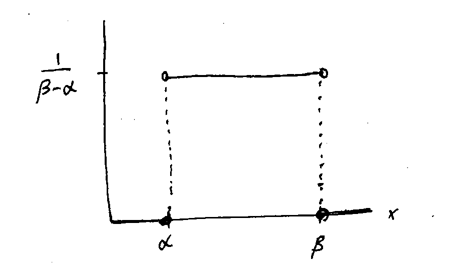
\includegraphics[width=\linewidth]{./images/unif.png}
\end{image}%
\tcblower
\end{figureptx}%
\begin{theorem}{mean and variance of continuous uniform.}{}{x:theorem:thm-cont-unif-mean}%
The mean and variance of the uniform distribution are given by%
\begin{equation*}
\mu = \dfrac{\alpha + \beta}{2}\text{ and }\sigma^2 =
\dfrac{1}{12}(\beta-\alpha)^2
\end{equation*}
%
\end{theorem}
\begin{inlineexercise}{continuous uniform moment-generating function.}{x:exercise:chall-cont-unif-mgf}%
Find the moment generating function of the continuous uniform distribution.%
\end{inlineexercise}
%
%
\typeout{************************************************}
\typeout{Exercises 4.3.1.1 Exercises}
\typeout{************************************************}
%
\begin{exercises-subsubsection}{Exercises}{}{Exercises}{}{}{g:exercises:idp140361459793376}
\begin{divisionexercise}{1}{Problem 6.1.}{}{g:exercise:idp140361459791712}%
Show that if a random vriable has a uniform density with parameters \(\alpha\) and \(\beta\), the probability that it will take on a value less than \(\alpha + p(\beta - \alpha)\) is \(p\).%
\end{divisionexercise}%
\begin{divisionexercise}{2}{Problem 6.3.}{}{g:exercise:idp140361459793504}%
If a random vriable has a uniform density with parameters \(\alpha\) and \(\beta\), find its distribution function.%
\end{divisionexercise}%
\end{exercises-subsubsection}
\end{subsectionptx}
%
%
\typeout{************************************************}
\typeout{Subsection 4.3.2 Exponential family}
\typeout{************************************************}
%
\begin{subsectionptx}{Exponential family}{}{Exponential family}{}{}{x:subsection:sub-exponential}
\begin{introduction}{}%
Two distributions, the exponential and chi-square, are special cases (i.e., parameterizations) of a very flexible distribution called the gamma.%
\end{introduction}%
We are at this point fairly familiar with the calculation of factorials. Factorials underlie our methods of counting, from permutations to combinations and partitions. For example, \(5! =
5\cdot4\cdot3\cdot2\cdot1 = 120\). What would it mean to ask for \(0.5!\)?%
\par
The gamma function allows us to generalize our concept of the factorial to noninteger, and even many nonpositive, values.%
\begin{definition}{gamma function.}{x:definition:def-gamma-func}%
The \terminology{gamma function} is given by%
\begin{equation*}
\Gamma(\alpha)
=\int_0^\infty y^{\alpha - 1}e^{-y}\,dy
\end{equation*}
where \(\alpha \gt
0\).%
\end{definition}
\begin{figureptx}{Graphs of the gamma function with a few key values.}{x:figure:fig-gamma}{}%
\begin{image}{0.25}{0.5}{0.25}%
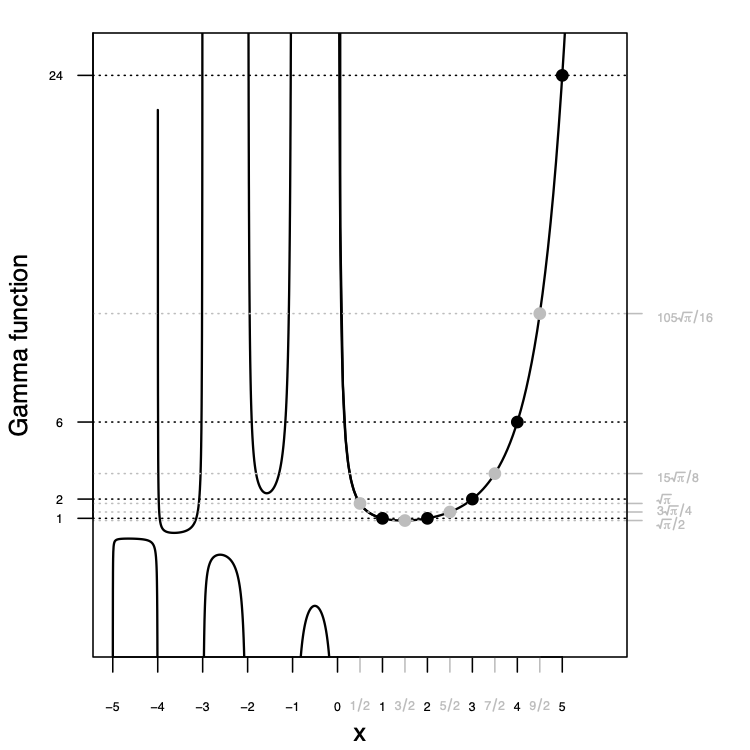
\includegraphics[width=\linewidth]{./images/gammaplot.png}
\end{image}%
\tcblower
\end{figureptx}%
\begin{tableptx}{\textbf{A table of common gamma function values.}}{x:table:tab-gammas}{}%
\centering
{\tabularfont%
\begin{tabular}{lllll}
\(\alpha\)&\(\Gamma(\alpha)\)&&\(\alpha\) (cont.)&\(\Gamma(\alpha)\) (cont.)\tabularnewline\hrulemedium
\(\sfrac{1}{2}\)&\(\sqrt{\pi}\)&&\(\sfrac{5}{2}\)&\(\sfrac{3\sqrt{\pi}}{4}\)\tabularnewline[0pt]
\(1\)&\(0! = 1\)&&\(3\)&\(2! = 2\)\tabularnewline[0pt]
\(\sfrac{3}{2}\)&\(\sfrac{\sqrt{\pi}}{2}\)&&\(\sfrac{7}{2}\)&\(\sfrac{15\sqrt{\pi}}{8}\)\tabularnewline[0pt]
\(2\)&\(1! = 1\)&&\(4\)&\(3! = 6\)
\end{tabular}
}%
\end{tableptx}%
\begin{definition}{gamma distribution.}{x:definition:def-cont-gamma}%
A continuous random variable \(\displaystyle X\) has a \terminology{gamma distribution} and is referred to as a \terminology{gamma random variable} if and only if its probability density is given by%
\begin{equation*}
f(x; \alpha, \beta) =
\begin{cases}\dfrac{1}{\beta^\alpha
\Gamma(\alpha)}x^{\alpha-1}e^{-\sfrac{x}{\beta}}, \amp \quad \text{
for }0 \lt x\\0, \amp \quad \text{elsewhere}\end{cases}
\end{equation*}
where \(\alpha, \beta \gt 0\).%
\end{definition}
\begin{figureptx}{A few folksy sketches of the gamma distribution.}{x:figure:fig-gamma-plots}{}%
\begin{image}{0.25}{0.5}{0.25}%
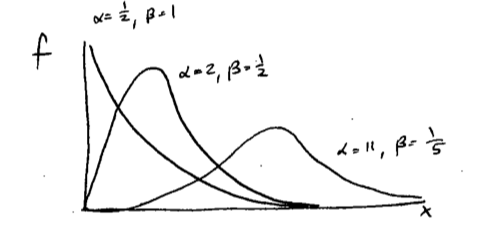
\includegraphics[width=\linewidth]{./images/gammas.png}
\end{image}%
\tcblower
\end{figureptx}%
\begin{theorem}{moments about the origin of the gamma.}{}{x:theorem:thm-cont-gamma-moments}%
The \(r^{\text{th}}\) moment about the origin of the gamma distribution is given by%
\begin{equation*}
\mu_r' = \dfrac{\beta^r\Gamma(\alpha+r)}{\Gamma(\alpha)}
\end{equation*}
%
\end{theorem}
\begin{theorem}{mean and variance of gamma.}{}{x:theorem:thm-cont-gamma-mean}%
The mean and variance of the gamma distribution are given by%
\begin{equation*}
\mu = \alpha\beta\text{ and }\sigma^2 = \alpha\beta^2
\end{equation*}
%
\end{theorem}
\begin{theorem}{moment-generating function of the gamma.}{}{x:theorem:thm-cont-gamma-mgf}%
The moment-generating function of the gamma distribution is given by%
\begin{equation*}
M_X(t) = (1-\beta t)^{-\alpha}
\end{equation*}
%
\end{theorem}
\begin{figureptx}{Derivation of the exponential distribution from a Poisson process (Part 1).}{x:figure:fig-pois-exp1}{}%
\begin{image}{0.1}{0.8}{0.1}%
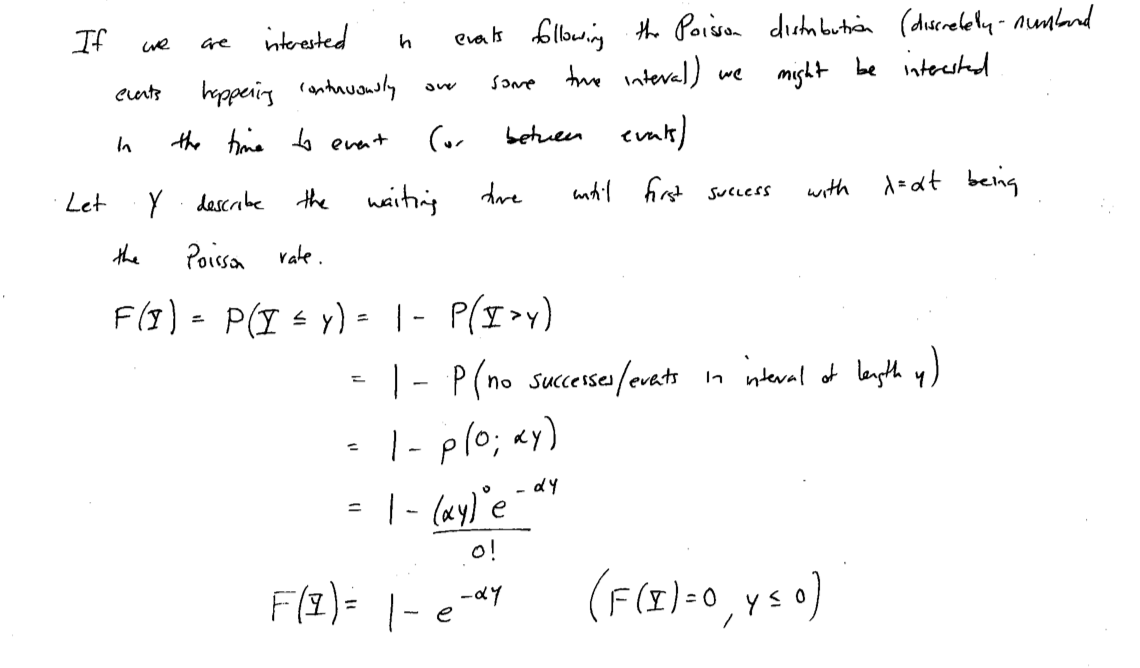
\includegraphics[width=\linewidth]{./images/poisson_exp.png}
\end{image}%
\tcblower
\end{figureptx}%
\begin{figureptx}{Derivation of the exponential distribution from a Poisson process (Part 2).}{x:figure:fig-pois-exp2}{}%
\begin{image}{0.1}{0.8}{0.1}%
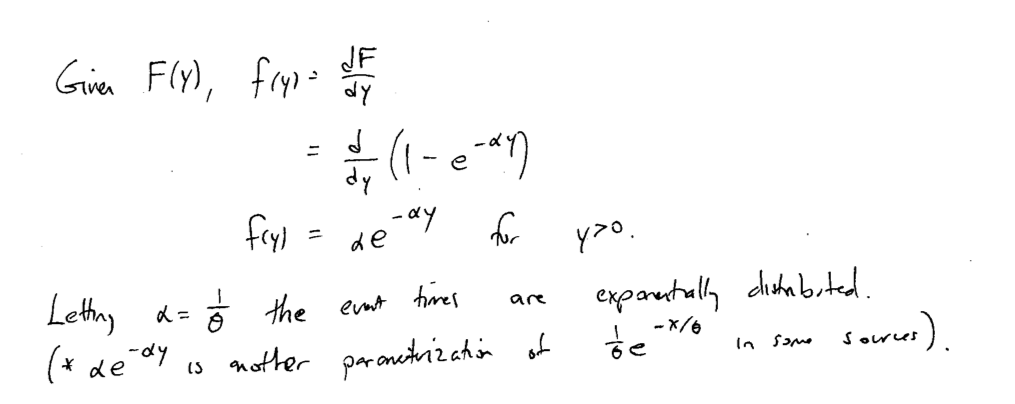
\includegraphics[width=\linewidth]{./images/poisson_exp2.png}
\end{image}%
\tcblower
\end{figureptx}%
\begin{definition}{exponential distribution.}{x:definition:def-cont-exp}%
A continuous random variable \(\displaystyle X\) has an \terminology{exponential distribution} and is referred to as an \terminology{exponential random variable} if and only if its probability density is given by%
\begin{equation*}
f(x; \theta) =
\begin{cases}\dfrac{1}{\theta}e^{-\sfrac{x}{\theta}}, \amp \quad \text{
for } 0 \lt x\\0, \amp \quad \text{elsewhere}\end{cases}
\end{equation*}
where \(\theta \gt 0\).%
\end{definition}
\begin{figureptx}{A few folksy sketches of the exponential distribution.}{x:figure:fig-exp-plots}{}%
\begin{image}{0.25}{0.5}{0.25}%
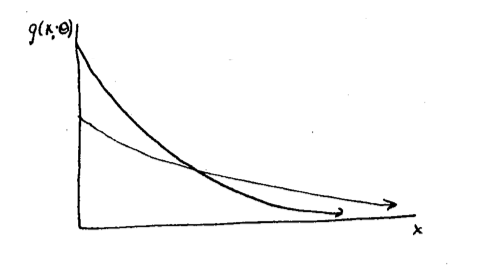
\includegraphics[width=\linewidth]{./images/exps.png}
\end{image}%
\tcblower
\end{figureptx}%
\begin{corollary}{mean and variance of exponential.}{}{x:corollary:cor-cont-exp-mean}%
The mean and variance of the exponential distribution are given by%
\begin{equation*}
\mu = \theta \text{ and }\sigma^2 = \theta^2
\end{equation*}
%
\end{corollary}
\begin{inlineexercise}{}{x:exercise:exer-exp-mean}%
By using the appropriate mathematical expectation, verify that the mean of the exponential distribution is as stated above.%
\end{inlineexercise}
\begin{remark}{}{x:remark:rmk-exp}%
The function used in \hyperref[x:example:ex-exponential]{Example~{\xreffont\ref{x:example:ex-exponential}}} and \hyperref[x:example:ex-exponential]{Example~{\xreffont\ref{x:example:ex-exponential}}} was an exponential distribution with \(\lambda = \sfrac{1}{\theta} = 3\).  Occasionally the exponential is parameterized by \(\lambda \gt 0\) with%
\begin{equation*}
f(x; \lambda) =
\begin{cases}\lambda e^{-\lambda x}, \amp \quad \text{
for } 0 \lt x\\0, \amp \quad \text{elsewhere}\end{cases}
\end{equation*}
%
\end{remark}
\begin{definition}{chi-suqare distribution.}{x:definition:def-cont-chi}%
A continuous random variable \(\displaystyle X\) has a \terminology{chi-square distribution} and is referred to as a chi-square random variable if and only if its probability density is given by%
\begin{equation*}
f(x; \nu) =
\begin{cases}\dfrac{1}{2^{\sfrac{\nu}{2}}
\Gamma(\sfrac{\nu}{2})}x^{\frac{\nu-2}{2}}e^{-\sfrac{x}{2}}, \amp \quad
\text{
for }0 \lt x\\0, \amp \quad \text{elsewhere}\end{cases}
\end{equation*}
where \(\nu\) is a parameter describing the \emph{number of degrees of freedom}.%
\end{definition}
%
%
\typeout{************************************************}
\typeout{Exercises 4.3.2.1 Exercises}
\typeout{************************************************}
%
\begin{exercises-subsubsection}{Exercises}{}{Exercises}{}{}{g:exercises:idp140361459844752}
\begin{divisionexercise}{1}{Problem 6.10(a).}{}{g:exercise:idp140361459847424}%
Find the probability that a random variable will exceed \(1\) if it has a gamma distribution with \(\alpha=2, \beta=3\).%
\end{divisionexercise}%
\begin{divisionexercise}{2}{Problem 6.23.}{}{g:exercise:idp140361459849440}%
A random variable \(X\) has a \emph{Weibull distribution} if and only if its probability density is given by%
\begin{equation*}
f(x; \alpha, \beta) =
\begin{cases}kx^{\beta-1}e^{-\alpha x^\beta}, \amp \quad
\text{
for }0 \lt x\\0, \amp \quad \text{elsewhere}\end{cases}
\end{equation*}
for \(\alpha, \beta \gt 0\).  Express \(k\) in terms of \(\alpha,
\beta\).%
\end{divisionexercise}%
See also: WeBWorK.%
\end{exercises-subsubsection}
\end{subsectionptx}
%
%
\typeout{************************************************}
\typeout{Subsection 4.3.3 Beta distribution}
\typeout{************************************************}
%
\begin{subsectionptx}{Beta distribution}{}{Beta distribution}{}{}{x:subsection:sub-beta}
\begin{introduction}{}%
In some applications, the beta distribution (which is a probability density itself) is actually used to described the distributions of \emph{other} probabilities.%
\end{introduction}%
\begin{definition}{Beta distribution.}{x:definition:def-cont-beta}%
A continuous random variable \(\displaystyle X\) has a \terminology{Beta distribution} and is referred to as a Beta random variable if and only if its probability density is given by%
\begin{equation*}
f(x; \alpha, \beta) =
\begin{cases}\dfrac{\Gamma(\alpha+\beta)}{\Gamma(\alpha)\Gamma(\beta)}x^
{\alpha-1}(1-x)^{\beta-1}, \amp \quad \text{
for }0 \lt x \lt 1\\0, \amp \quad \text{elsewhere}\end{cases}
\end{equation*}
where \(\alpha, \beta \gt 0\).%
\end{definition}
\begin{figureptx}{A few folksy sketches of the beta distribution. Notice that for \(\alpha = \beta = 0.5\), the PDF has vertical asymptotes at \(x =
0, 1\). For \(\alpha = \beta = 2\), the PDF simplifies to \(f(x; 2, 2) =
6x(1-x)\).}{x:figure:fig-beta-plots}{}%
\begin{image}{0.25}{0.5}{0.25}%
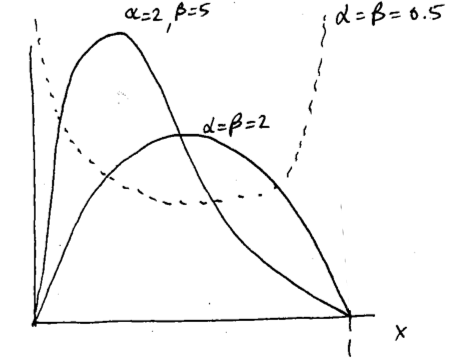
\includegraphics[width=\linewidth]{./images/betas.png}
\end{image}%
\tcblower
\end{figureptx}%
\begin{remark}{}{x:remark:rmk-beta}%
The function used in \hyperref[x:example:ex-poly]{Example~{\xreffont\ref{x:example:ex-poly}}} was a beta distribution with \(\alpha=\beta=5\).%
\end{remark}
%
%
\typeout{************************************************}
\typeout{Exercises 4.3.3.1 Exercises}
\typeout{************************************************}
%
\begin{exercises-subsubsection}{Exercises}{}{Exercises}{}{}{g:exercises:idp140361459860320}
\begin{divisionexercise}{1}{Problem 6.25(a).}{}{g:exercise:idp140361459863424}%
Verify that the integral of the beta density function from \(-\infty\) to \(\infty\) equals \(1\) if it has a gamma distribution with \(\alpha=2, \beta=4\).%
\end{divisionexercise}%
See also: WeBWorK.%
\end{exercises-subsubsection}
\end{subsectionptx}
%
%
\typeout{************************************************}
\typeout{Subsection 4.3.4 Normal distribution}
\typeout{************************************************}
%
\begin{subsectionptx}{Normal distribution}{}{Normal distribution}{}{}{x:subsection:sub-normal}
...%
\begin{definition}{Normal distribution.}{x:definition:def-cont-normal}%
A continuous random variable \(\displaystyle X\) has a \terminology{normal distribution} and is referred to as a normal random variable if and only if its probability density is given by%
\begin{equation*}
n(x; \mu, \sigma) = \dfrac{1}{\sigma\sqrt{2\pi}}
e^{-\dfrac{1}{2}\left(\dfrac{x-\mu}{\sigma}\right)^2}, \quad \text{
for }-\infty \lt x \lt \infty
\end{equation*}
where \(\sigma \gt 0\).%
\end{definition}
\begin{theorem}{mean and variance of normal.}{}{x:theorem:thm-cont-normal-mean}%
The mean and variance of the normal distribution are given by%
\begin{equation*}
\mu = \mu\text{ and }\sigma^2 = \sigma^2
\end{equation*}
%
\end{theorem}
\begin{theorem}{moment-generating function of the normal.}{}{x:theorem:thm-cont-normal-mgf}%
The moment-generating function of the normal distribution is given by%
\begin{equation*}
M_X(t) = e^{\mu t + \sfrac{1}{2}\sigma^2t^2}
\end{equation*}
%
\end{theorem}
\begin{remark}{}{x:remark:rmk-params-normal}%
The PDF is parameterized by \(\mu\) and \(\sigma = \sqrt{\sigma^2} =
\sqrt{\operatorname{Var}(X)}\).%
\end{remark}
\begin{corollary}{}{}{x:corollary:corr-std-normal}%
The \terminology{standard normal} has \(\mu = 0\) and \(\sigma =
1\) and is given by%
\begin{equation*}
f(x; \mu = 0, \sigma = 1) =
\dfrac{1}{\sqrt{2\pi}}
e^{-\dfrac{1}{2}x^2}, \quad \text{
for }-\infty \lt x \lt \infty
\end{equation*}
%
\end{corollary}
\begin{remark}{}{x:remark:rmk-table-std-normal}%
It is the standard normal distribution for which areas under the curve given by%
\begin{equation*}
\int_0^z \dfrac{1}{\sqrt{2\pi}}
e^{-\dfrac{1}{2}x^2}\,dx
\end{equation*}
are tabulated.%
\begin{figureptx}{Table of standard normal probabilities. The highlighted entry \(''0.2224''\) corresponds to the probability \(P(z \lt 0.59) =
0.2224\) and gives the area under the graph of the standard normal curve between \(z=0\) and \(z =0.59\).}{x:figure:fig-std-tab}{}%
\begin{image}{0.1}{0.8}{0.1}%
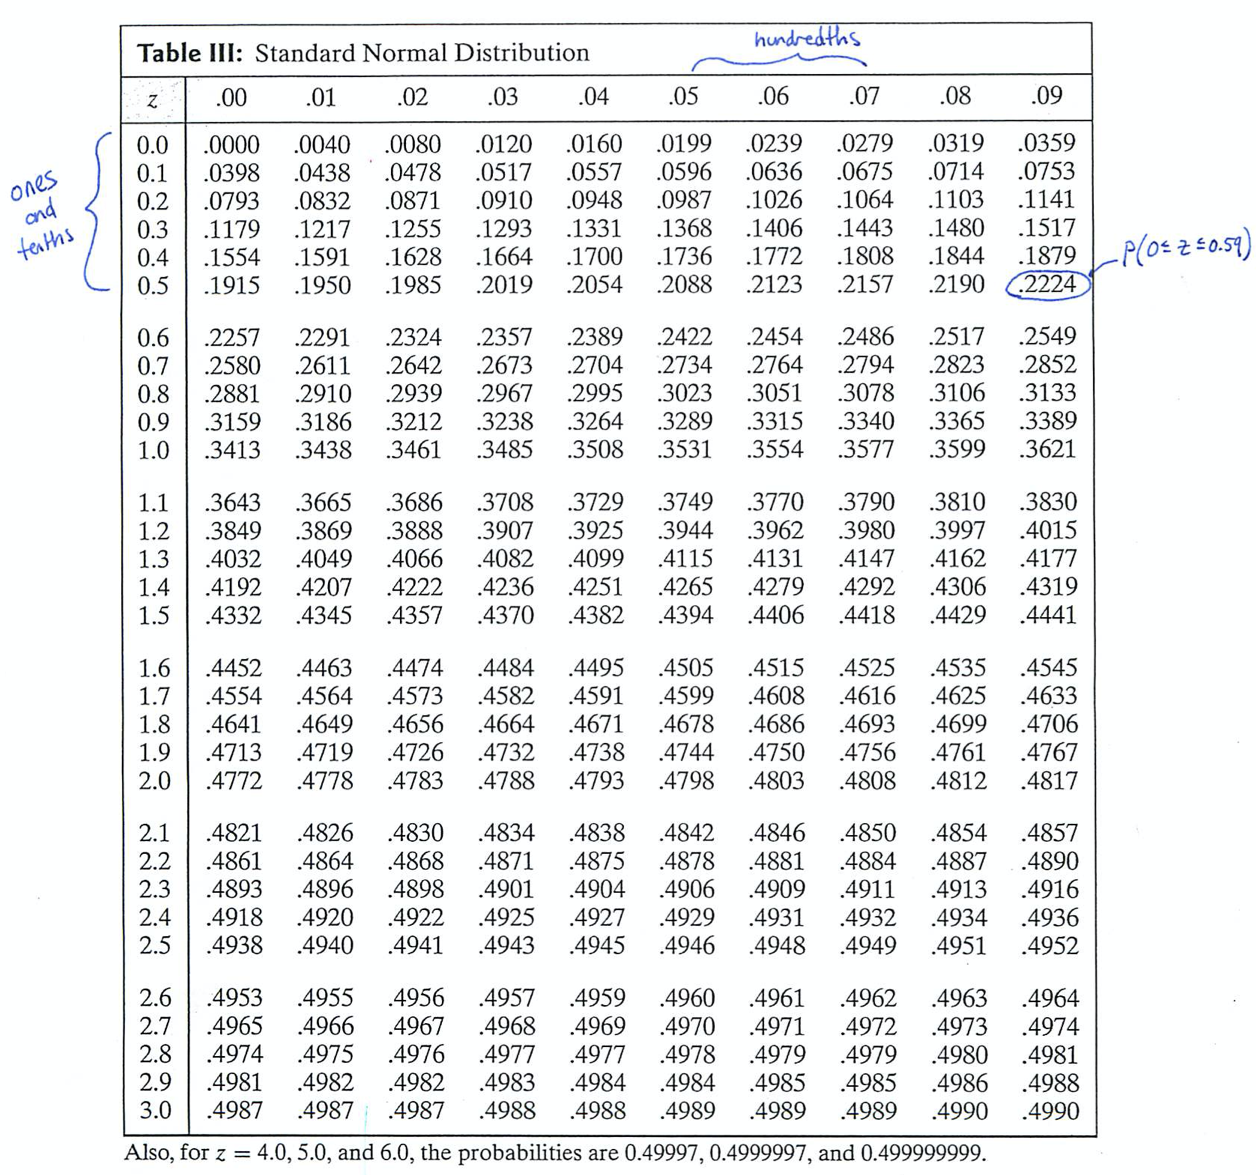
\includegraphics[width=\linewidth]{./images/ztab.png}
\end{image}%
\tcblower
\end{figureptx}%
Other areas can be calculated by symmetry.%
\end{remark}
\begin{theorem}{transforming to standard normal.}{}{x:theorem:thm-cont-std-normal}%
If \(X\) has a normal distribution with \(\mu\) and \(\sigma\), then \(\displaystyle Z = \dfrac{X - \mu}{\sigma}\) has the standard normal distribution.%
\end{theorem}
A few special probabilities for the standard normal are given by%
\begin{enumerate}
\item{}\(\displaystyle P(-\infty \lt z \lt 0) = 0.5\)%
\item{}\(\displaystyle P(0 \lt z \lt \infty) = 0.5\)%
\item{}\(\displaystyle P(-\infty \lt z \lt \infty) = 1\)%
\item{}\(\displaystyle P(-a \lt z \lt a) = 2\cdot P(0 \lt z \lt a)\)%
\end{enumerate}
%
\begin{example}{probabilities from the standard normal.}{x:example:ex-std-norm-probs}%
Find the following probabilities from the standard normal distribution.%
\begin{enumerate}
\item{}\(\displaystyle P(|z|\lt 0.3)\)%
\item{}\(\displaystyle P(0.3 \lt z \lt 0.6)\)%
\item{}\(\displaystyle P(0.6 \lt z)\)%
\end{enumerate}
%
\textbf{\blocktitlefont Solution}.\quad{}To find \(P(|z|\lt 0.3)\), we must first find \(P(0 \lt z \lt
0.3)\). Once we have that, we can double this value by symmetry of the PDF.%
\begin{figureptx}{Area under the curve corresponding to desired probability.}{x:figure:fig-std-norm1}{}%
\begin{image}{0.25}{0.5}{0.25}%
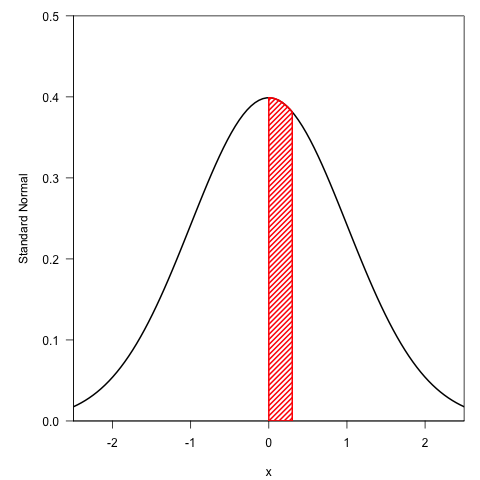
\includegraphics[width=\linewidth]{./images/std_norm1.png}
\end{image}%
\tcblower
\end{figureptx}%
Now to find \(P(|z|\lt 0.3)\), we have the following image. By table we have that \(P(0 \lt z \lt 0.3) = 0.1179\), so \(P(|z|\lt 0.3) = 2(0.1179) = 0.2358\).  For simplicity we will use an equality here, even though the tabulated areas are numerical approximations.%
\begin{figureptx}{Area under the curve corresponding to desired probability.}{x:figure:fig-std-norm2}{}%
\begin{image}{0.25}{0.5}{0.25}%
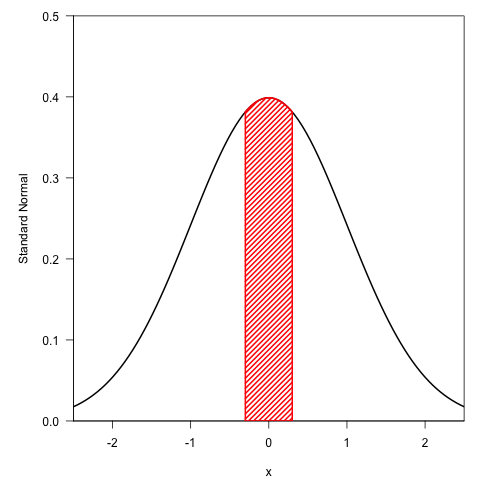
\includegraphics[width=\linewidth]{./images/std_norm2.png}
\end{image}%
\tcblower
\end{figureptx}%
Now to find \(P(0.3 \lt z \lt 0.6)\), we have the following image. To solve this problem we find the area from \(z=0\) to \(z=0.6\), then subtract the area from \(z=0\) to \(z=0.3\).%
\begin{figureptx}{Area under the curve corresponding to desired probability.}{x:figure:fig-std-norm3}{}%
\begin{image}{0.25}{0.5}{0.25}%
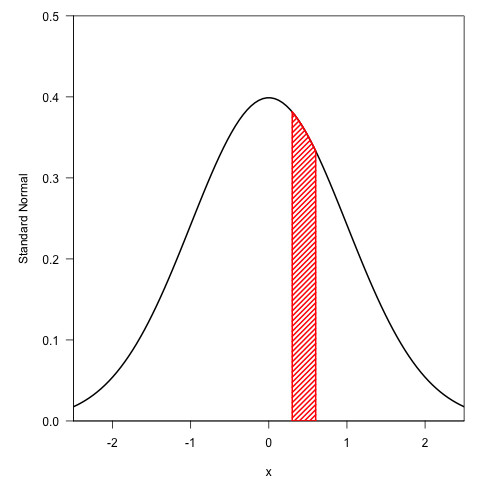
\includegraphics[width=\linewidth]{./images/std_norm3.png}
\end{image}%
\tcblower
\end{figureptx}%
Now to find \(P(0.6 \lt z)\), we have the following image.  To solve this problem we find the area from \(z=0\) to \(z=0.6\), then subtract this from the area under the entire right half of the curve.  So \(P(0.6 \lt z)\) = 0.5 - 0.2257 = 0.2743%
\begin{figureptx}{Area under the curve corresponding to desired probability.}{x:figure:fig-std-norm4}{}%
\begin{image}{0.25}{0.5}{0.25}%
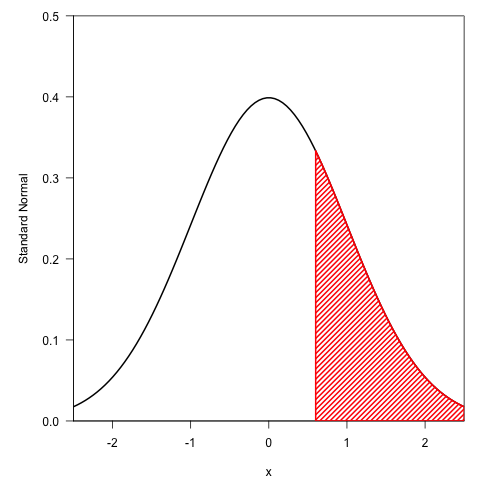
\includegraphics[width=\linewidth]{./images/std_norm4.png}
\end{image}%
\tcblower
\end{figureptx}%
\end{example}
\begin{example}{probabilities from the standard normal.}{x:example:ex-std-norm-probs2}%
Find the associated standard normal random variable \(Z\) for a normal random variable \(X\) with \(\mu = 19.7\) and \(\sigma = 9.1\) and use it to calculate the probability that \(Z \gt 25\).%
\textbf{\blocktitlefont Hint}.\quad{}Transform to \(Z\) then use the table.%
\end{example}
%
%
\typeout{************************************************}
\typeout{Exercises 4.3.4.1 Exercises}
\typeout{************************************************}
%
\begin{exercises-subsubsection}{Exercises}{}{Exercises}{}{}{g:exercises:idp140361459910304}
\begin{divisionexercise}{1}{Problem 6.31.}{}{g:exercise:idp140361459911536}%
Show that the normal distribution has a relative maximum at \(x =
\mu\) and inflection points at \(x = \mu \pm \sigma\).%
\end{divisionexercise}%
See also: WeBWorK.%
\end{exercises-subsubsection}
\end{subsectionptx}
%
%
\typeout{************************************************}
\typeout{Subsection 4.3.5 Normal approximation to the binomial distribution}
\typeout{************************************************}
%
\begin{subsectionptx}{Normal approximation to the binomial distribution}{}{Normal approximation to the binomial distribution}{}{}{x:subsection:sub-normal-approx}
\begin{introduction}{}%
...%
\end{introduction}%
\begin{theorem}{normal approximation to the binomial.}{}{x:theorem:thm-cont-normal-binom}%
If \(X\) has a binomial distribution with parameters \(n\) and \(\theta\), then the moment-generating function of \(\dfrac{X-n\theta}{\sqrt{n\theta(1-\theta)}}\) approaches \(M_X(t) =
\underbrace{e^{\sfrac{1}{2}t^2}}_{\text{std. normal}}\) as \(n\to\infty\).%
\end{theorem}
This is because of a \(1:1\) correspondence between moment-generating functions and PMFs\slash{}PDFs and the (unstated) fact that if \(M_X(t) \to M_Y(t)\), then \(\text{the distribution of }X
\to\text{ the distribution of }Y\).%
\par
The approximation is true as \(n\to\infty\) and can be used when both \(n\theta, n(1-\theta) \gt 5\).  This is theoretically important and was of great historical importance, but is less practically important%
\par
Since calculating densities reqires intervals, a \emph{continuity correction} represents the binomial integer \(k\) by the \emph{standard normal} interval \((k-\sfrac{1}{2},
k+\sfrac{1}{2})\) for the purposes of integration.%
%
%
\typeout{************************************************}
\typeout{Exercises 4.3.5.1 Exercises}
\typeout{************************************************}
%
\begin{exercises-subsubsection}{Exercises}{}{Exercises}{}{}{g:exercises:idp140361459923488}
\begin{divisionexercise}{1}{Problem 6.75(a, b).}{}{g:exercise:idp140361459923616}%
Make the normal approximation to \(b(1; 150, 0.05)\). Is the approximation reasonable? How does it compare to a (rounded) true value of \(b(1;
150, 0.05) = 0.0036\)?%
\end{divisionexercise}%
See also: WeBWorK.%
\end{exercises-subsubsection}
\end{subsectionptx}
\end{sectionptx}
\end{chapterptx}
%
%
\typeout{************************************************}
\typeout{Chapter 5 Multivariate Probability Distributions and Densities}
\typeout{************************************************}
%
\begin{chapterptx}{Multivariate Probability Distributions and Densities}{}{Multivariate Probability Distributions and Densities}{}{}{x:chapter:chap-multi}
\begin{introduction}{}%
We will study the theory of multivariable discrete and continuous random variables, their mathematical expectations, and specific examples of densities from practice. We will largely repeat the ideas of \hyperref[x:chapter:chap-discrete]{Chapter~{\xreffont\ref{x:chapter:chap-discrete}}} and \mono{[cross-reference to target(s) \textquotedbl{}chap-cont\textquotedbl{} missing]}, but this time in higher dimensions.%
\end{introduction}%
%
%
\typeout{************************************************}
\typeout{Section 5.1 Multivariate discrete random variables}
\typeout{************************************************}
%
\begin{sectionptx}{Multivariate discrete random variables}{}{Multivariate discrete random variables}{}{}{x:section:section-multivariate-discrete-probability}
\begin{introduction}{}%
Some words.%
\end{introduction}%
%
%
\typeout{************************************************}
\typeout{Subsection 5.1.1 Multivariate, marginal, and conditional distributions}
\typeout{************************************************}
%
\begin{subsectionptx}{Multivariate, marginal, and conditional distributions}{}{Multivariate, marginal, and conditional distributions}{}{}{x:subsection:sub-multi-variable}
\begin{introduction}{}%
See sections 3.5, 3.6, 3.7. Recommended problems: (pg 101) 42, 44, 45, 49, 53, 54%
\end{introduction}%
\begin{definition}{joint probability distribution.}{x:definition:def-joint-probability-distribution-3-6}%
If \(\displaystyle X\) and \(\displaystyle Y\) are discrete random variables, the function given by \(\displaystyle f(x,y) = P(X=x,
Y=y)\) for each pair of values \(\displaystyle (x,y)\) within the range of \(\displaystyle X\) and \(\displaystyle Y\) is called the \terminology{joint probability distribution} of \(\displaystyle X\) and \(\displaystyle Y\).%
\end{definition}
\begin{theorem}{conditions for a joint probability distribution.}{}{x:theorem:thm-3-7}%
A bivariate function can serve as a joint probability distribution for a pair of discrete random variables \(\displaystyle X\) and \(\displaystyle Y\) if and only if its values, \(\displaystyle f(x,
y)\), satisfy the conditions%
\begin{enumerate}
\item{}\(\displaystyle f(x, y) \ge 0\) for each pair of values \(\displaystyle (x, y)\) within its domain;%
\item{}\(\displaystyle \sum_x\sum_y f(x, y) = 1\) where the double summation extends over all possible pairs \(\displaystyle (x,
y)\).%
\end{enumerate}
%
\end{theorem}
\begin{definition}{joint distribution function.}{x:definition:def-joint-distribution-function-3-7}%
If \(\displaystyle X\) and \(\displaystyle Y\) are discrete random variables, the function given by%
\begin{equation*}
F(x, y) = P(X \le x, Y \le y) =
\sum_{s\le x} \sum_{t\le y} f(s, t) \text{ for } \infty \lt x, y \lt
\infty
\end{equation*}
where \(\displaystyle f(s, t)\) is the value of the joint probability distribution of \(\displaystyle X\) and \(\displaystyle
Y\) at \(\displaystyle (s, t)\), is called the \terminology{joint distribution function} or \terminology{joint cumulative distribution} of \(\displaystyle X\) and \(\displaystyle
Y\).%
\end{definition}
\begin{definition}{marginal distribution.}{x:definition:def-marginal-distribution-3-10}%
If \(\displaystyle X\) and \(\displaystyle Y\) are discrete random variables and \(\displaystyle f(x, y)\) is the value of their joint probability distribution at \(\displaystyle (x, y)\), the function given by%
\begin{equation*}
g(x) = \sum_y f(x, y)
\end{equation*}
for each \(\displaystyle x\) within the range of \(\displaystyle X\) is called the \terminology{marginal distribution} of \(\displaystyle X\). Correspondingly, the function given by%
\begin{equation*}
h(y) = \sum_x f(x, y)
\end{equation*}
for each \(\displaystyle y\) within the range of \(\displaystyle Y\) is called the \terminology{marginal distribution} of \(\displaystyle Y\).%
\end{definition}
\begin{definition}{conditional distribution.}{x:definition:def-conditional-distribution-3-10}%
\terminology{conditional distribution}%
\begin{equation*}
f(x|y) = \dfrac{f(x, y)}{h(y)}, h(y)\ne 0
\end{equation*}
%
\begin{equation*}
w(y|x) = \dfrac{f(x, y)}{g(x)}, g(x)\ne 0
\end{equation*}
%
\end{definition}
\end{subsectionptx}
%
%
\typeout{************************************************}
\typeout{Exercises 5.1.2 Exercises}
\typeout{************************************************}
%
\begin{exercises-subsection}{Exercises}{}{Exercises}{}{}{g:exercises:idp140361424873952}
\begin{divisionexercise}{1}{Problem 3.42.}{}{g:exercise:idp140361424873392}%
If the values of the joint probability distribution of \textbackslash{}(X\textbackslash{}) and \textbackslash{}(Y\textbackslash{}) are shown below,%
\begin{equation*}
\begin{aligned}[t]
P[x=0, y=0] \amp = \frac{1}{12}\\
P[x=1, y=0] \amp = \frac{1}{6}\\
P[x=2, y=0] \amp = \frac{1}{24}\\
P[x=0, y=1] \amp = \frac{1}{4}\\
P[x=1, y=1] \amp = \frac{1}{4}\\
P[x=2, y=1] \amp = \frac{1}{40}\\
P[x=0, y=2] \amp = \frac{1}{8}\\
P[x=1, y=2] \amp = \frac{1}{20}\\
P[x=0, y=3] \amp = \frac{1}{120}\\
\end{aligned}
\end{equation*}
find%
\begin{enumerate}[label=(\alph*)]
\item{}(b) \(P(X = 0, 1\le Y \lt 3)\)%
\item{}(c) \(P(X + Y \le 1)\)%
\item{}(d) \(P(X \gt Y)\)%
\end{enumerate}
%
\end{divisionexercise}%
\begin{divisionexercise}{2}{Problem 3.44.}{}{g:exercise:idp140361424849552}%
If the joint probability distribution of \(X\) and \(Y\) is given by%
\begin{equation*}
f(x, y) = c(x^2+y^2) \text{ for } x=0, 3; y=0, 1, 2
\end{equation*}
find the value of \(c\).%
\end{divisionexercise}%
\begin{divisionexercise}{3}{Problem 3.45.}{}{g:exercise:idp140361424826432}%
With references to the previous problem find%
\begin{enumerate}[label=(\alph*)]
\item{}\(\displaystyle P(X\le 1, Y \gt 2)\)%
\item{}\(\displaystyle P(X=0, Y\le 2)\)%
\item{}\(\displaystyle P(X +Y \gt 2)\)%
\end{enumerate}
%
\end{divisionexercise}%
\begin{divisionexercise}{4}{Problem 3.70.}{}{g:exercise:idp140361424787856}%
With reference to 3.42, find%
\begin{enumerate}[label=(\alph*)]
\item{}the marginal distribution of \(X\)%
\item{}the marginal distribution of \(X\)%
\item{}the conditional distribution of \(X\) given \(Y=1\)%
\item{}the conditional distribution of \(Y\) given \(X=0\)%
\end{enumerate}
%
\end{divisionexercise}%
\end{exercises-subsection}
%
%
\typeout{************************************************}
\typeout{Subsection 5.1.3 }
\typeout{************************************************}
%
\begin{subsectionptx}{}{}{}{}{}{x:subsection:sub-expectation-multi}
\begin{theorem}{expected value of joint random variables.}{}{x:theorem:thm-expected-value-joint-random-variables-4-4}%
If \(X\) and \(Y\) are discrete random variables and \(\displaystyle f(x, y)\) is the value of their joint probability distribution at \(\displaystyle (x, y)\), the expected value of \(\displaystyle g(X, Y)\) is given by%
\begin{equation*}
E[g(X, Y)] = \sum_x \sum_y g(x, y)\cdot f(x,y)
\end{equation*}
%
\end{theorem}
\begin{theorem}{expected value of a linear combination of random variables.}{}{x:theorem:thm-4-5}%
If \(\displaystyle c_1, c_2, \dots, c_n\) are constants, then%
\begin{equation*}
E\left[\sum_{i=1}^n c_i g_i(X_1, X_2, \dots, X_k)\right] =
\sum_{i=1}^n c_i E\left[g_i(X_1, X_2, \dots, X_k)\right]
\end{equation*}
%
\end{theorem}
\end{subsectionptx}
%
%
\typeout{************************************************}
\typeout{Subsection 5.1.4 Product moments}
\typeout{************************************************}
%
\begin{subsectionptx}{Product moments}{}{Product moments}{}{}{x:subsection:sub-product-moments}
See section 4.6.%
\begin{definition}{product moments about the origin.}{x:definition:def-product-moments-origin-4-7}%
The \terminology{\(\displaystyle r^\text{th}\) and \(\displaystyle
s^\text{th}\) product moment about the origin} of the random variables \(X\) and \(Y\), denoted by \(\displaystyle \mu_{r,s}\), is the expected value of \(\displaystyle X^rY^s\); symbolically%
\begin{equation*}
\mu_{r,s}'=E[X^rY^s] = \sum_x\sum_y x^r y^s\cdot f(x, y)
\end{equation*}
\(\displaystyle r = 0,1,2, \dots\) and \(\displaystyle s = 0,1,2,
\dots\) when \(X\) and Y are discrete.%
\end{definition}
Special cases of product moments are \(\displaystyle \mu_{1,0}' =
E[X^1Y^0] = E[X] = \mu_X\) and \(\displaystyle \mu_{0,1}' = E[X^0Y^1]
= E[Y] = \mu_Y\).%
\par
As complicated as the definitions of the product moments may be, they lead to a way to define and calculate the very important concept of covariance.%
\begin{itemize}[label=\textbullet]
\item{}If we have a high probability of large \(X\) paired with large \(Y\) and small \(\displaystyle
X\) paired with small \(Y\), \(\displaystyle
\operatorname{cov}(X,Y) \gt 0\)%
\item{}If we have a high probability of large \(X\) paired with small \(Y\) and small \(\displaystyle
X\) paired with large \(Y\), \(\displaystyle
\operatorname{cov}(X,Y) \lt 0\)%
\end{itemize}
%
\begin{definition}{product moments about the mean.}{x:definition:def-product-moments-mean-4-8}%
The \terminology{\(\displaystyle r^\text{th}\) and \(\displaystyle
s^\text{th}\) product moment about the mean} of the random variables \(X\) and \(Y\), denoted by \(\displaystyle \mu_{r,s}'\), is the expected value of \(\displaystyle (X-\mu_X)^r(Y-\mu_Y)^s\); symbolically%
\begin{equation*}
\mu_{r,s}=E[(X-\mu_X)^r(Y-\mu_Y)^s] = \sum_x\sum_y (x-\mu_X)^r
(y-\mu_Y)^s\cdot f(x, y)
\end{equation*}
\(\displaystyle r = 0,1,2, \dots\) and \(\displaystyle s = 0,1,2, \dots\) when \(X\) and Y are discrete.%
\end{definition}
\begin{definition}{covariance.}{x:definition:def-covariance-4-9}%
\(\displaystyle \mu_{1,1}\) is called the \terminology{covariance} of \(X\) and \(Y\), and it is denoted by \(\displaystyle \sigma_{XY}\) or \(\displaystyle
\operatorname{cov}(X, Y)\), or \(\displaystyle C(X, Y)\).%
\end{definition}
\begin{theorem}{covariance from moments about the origin.}{}{x:theorem:thm-4-11}%
\(\displaystyle \sigma_{XY} = \mu_{1,1}' - \mu_X \mu_Y\)%
\end{theorem}
\begin{theorem}{independence and covariance.}{}{x:theorem:thm-4-12}%
If \(X\) and \(Y\) are independent, then%
\begin{equation*}
\displaystyle E[XY] = E[X]\cdot E[Y]
\end{equation*}
and \(\displaystyle \sigma_{XY} = 0\).%
\end{theorem}
\begin{remark}{}{x:remark:rmrk-4-12}%
In terms of moments,%
\begin{equation*}
\displaystyle\mu_{1,1}' = \mu_{1,0}'\cdot \mu_{0,1}'
\end{equation*}
\end{remark}
\begin{theorem}{product moments of independent random variables.}{}{x:theorem:thm-4-13}%
If \(\displaystyle X_1, X_2, \dots, X_n\) are independent, then \(\displaystyle E[X_1X_2\cdots X_n] = E[X_1]\cdot
E[X_2]\cdot\cdots\cdot E[X_n]\).%
\end{theorem}
Independence means covariance is zero, but covariances of zero does not mean independence.%
\end{subsectionptx}
%
%
\typeout{************************************************}
\typeout{Exercises 5.1.5 Exercises}
\typeout{************************************************}
%
\begin{exercises-subsection}{Exercises}{}{Exercises}{}{}{g:exercises:idp140361424551664}
\begin{divisionexercise}{1}{Problem 4.41.}{}{g:exercise:idp140361424551184}%
If \(X\) and \(Y\) have the joint probability distribution \(f(x, y) = \dfrac{1}{4}\) for \((-3, -5)\),  \((-1, -1)\), \((1, 1)\),  \((3, 5)\), find \(\operatorname{cov}(X, Y)\).%
\end{divisionexercise}%
\begin{divisionexercise}{2}{Problem 4.45.}{}{g:exercise:idp140361424534208}%
If \(X\) and \(Y\) have the joint probability distribution \(f(-1, 0) = 0\),  \(f(-1, 1) = \dfrac{1}{4}\), \(f(0, 0) = \dfrac{1}{6}\), \(f(1, 0) = \dfrac{1}{12}\), \(f(1,
1) = \dfrac{1}{2}\) show that%
\begin{enumerate}[label=(\alph*)]
\item{}\(\operatorname{cov}(X, Y) = 0\);%
\item{}the two random variables are not independent.%
\end{enumerate}
%
\end{divisionexercise}%
\end{exercises-subsection}
%
%
\typeout{************************************************}
\typeout{Subsection 5.1.6 Moments of linear combinations of random variables}
\typeout{************************************************}
%
\begin{subsectionptx}{Moments of linear combinations of random variables}{}{Moments of linear combinations of random variables}{}{}{x:subsection:sub-moments-linear-combinations}
\begin{introduction}{}%
See section 4.7. Recommended problems: 4.7-8 (pg 158) 48, 49, 57%
\end{introduction}%
\begin{theorem}{variance.}{}{x:theorem:thm-4-14}%
If \(\displaystyle X_1, X_2, \dots, X_n\) are random variables and \(\displaystyle Y = \sum_{i=1}^n a_iX_i\) where \(\displaystyle
a_1, a_2, \dots, a_n\) are constants, then%
\begin{equation*}
E[Y] = \sum_{i=1}^n
a_iE[X_i]
\end{equation*}
and%
\begin{equation*}
\operatorname{var}[Y] = \sum_{i=1}^n a_i^2
\operatorname{var}[X_i] + 2 \mathop{\sum \sum}_{i \lt j} a_i
a_j\operatorname{cov}[X_i,X_j]\text{.}
\end{equation*}
%
\end{theorem}
\begin{corollary}{variance of independent random variables.}{}{x:corollary:cor-4-3}%
If \(\displaystyle X_1, X_2, \dots, X_n\) are independent random variables and \(\displaystyle Y = \sum_{i=1}^n a_iX_i\) where \(\displaystyle a_1, a_2, \dots, a_n\) are constants, then%
\begin{equation*}
\operatorname{var}[Y] = \sum_{i=1}^n
a_i^2\operatorname{var}[X_i]
\end{equation*}
%
\end{corollary}
\begin{example}{covariances of linear combinations.}{x:example:ex-var-covar}%
Consider three random variables \(X\), \(Y\), and \(Z\) with \(\mu_X = 2\), with \(\mu_Y = -3\), with \(\mu_Z = 4\); with \(\sigma_X^2 = 1\), \(\sigma_Y^2 = 5\), \(\sigma_Z^2 =
2\); and \(\operatorname{cov}(X, Y) = -2\), \(\operatorname{cov}(X, Z) =
-1\), and \(\operatorname{cov}(Y, Z) = 1\).%
\par
Find \(\mu_W\) and \(\operatorname{var}(W) = \sigma_W^2\) for \(W = 3X-Y+2Z\).%
\textbf{\blocktitlefont Solution}.\quad{}First, \(\mu_W = (3)\mu_X + (-1)\mu_Y + (2)\mu_Z = 17\).%
\par
We could apply the theorem directly, but we can do this more directly with linear algebra. The idea is that we can picture the linear combination \(W = 3X-Y+2Z\) as%
\begin{equation*}
W =
\left[\begin{array}{ccc}3 \amp -1 \amp
2\end{array}\right]\cdot\left[\begin{array}{c}X \\Y\\
Z\end{array}\right] = (3)X + (-1)Y + (2)Z
\end{equation*}
%
\par
Let \(a\) be the row vector \(a = \left[\begin{array}{ccc}3 \amp -1
\amp 2\end{array}\right]\), its transpose be the column vector \(a^T\), and the matrix \(\Sigma\) be defined as follows,%
\begin{equation*}
\Sigma = \left[\begin{array}{ccc}
1 \amp -2 \amp -1\\
-2 \amp 5 \amp 1\\
-1 \amp 1 \amp 2
\end{array}\right]
\end{equation*}
%
\par
This approach can be justified by expanding the sums in \hyperref[x:theorem:thm-4-14]{Theorem~{\xreffont\ref{x:theorem:thm-4-14}}} with a sum of 2 random variables.%
\par
We can calculate the variance of \(W\) by \(\operatorname{var}(W)
= a\Sigma a^T\). Specifically,%
\begin{equation*}
a \Sigma a^T = \left[\begin{array}{ccc}3 \amp -1 \amp
2\end{array}\right]\cdot\left[\begin{array}{ccc}
1 \amp -2 \amp -1\\
-2 \amp 5 \amp 1\\
-1 \amp 1 \amp 2
\end{array}\right]\cdot\left[\begin{array}{c}3 \\-1\\
2\end{array}\right]
\end{equation*}
%
\par
Notice \(Sigma\) is symmetric and that the covariances lie in order along the main diagonal and the variances off-diagonal.%
\par
Multiplying the square matrix and column vector first, we have%
\begin{equation*}
a \Sigma a^T = \left[\begin{array}{ccc}3 \amp -1 \amp
2\end{array}\right]\cdot\left[\begin{array}{c}3 \\-9\\
0\end{array}\right]
\end{equation*}
%
\par
And finally, \(a \Sigma a^T = 18\).%
\end{example}
\begin{theorem}{covariance of two linear combinations.}{}{x:theorem:thm-4-15}%
If \(\displaystyle X_1, X_2, \dots, X_n\) are random variables and \(\displaystyle Y_1 = \sum_{i=1}^n a_i X_i \text{ and } Y_2 =
\sum_{i=1}^n b_iX_i\) where \(\displaystyle a_1, a_2, \dots, a_n,
b_1, b_2, \dots, b_n\) are constants, then%
\begin{equation*}
\operatorname{cov}[Y_1,
Y_2] = \sum_{i=1}^n a_i b_i\operatorname{var}[X_i] + \mathop{\sum
\sum}_{i \lt j} (a_ib_j + a_jb_i)\operatorname{cov}[X_i,X_j]\text{.}
\end{equation*}
%
\end{theorem}
\begin{corollary}{}{}{x:corollary:cor-4-3b}%
If \(\displaystyle X_1, X_2, \dots, X_n\) are independent random variables and \(\displaystyle Y_1 = \sum_{i=1}^n a_iX_i \text{ and } Y_2 =
\sum_{i=1}^n b_iX_i\), then%
\begin{equation*}
\operatorname{cov}[Y_1, Y_2] =
\sum_{i=1}^n a_i b_i\operatorname{var}[X_i]
\end{equation*}
%
\end{corollary}
 The same logic used in \hyperref[x:example:ex-var-covar]{Example~{\xreffont\ref{x:example:ex-var-covar}}} allows us to compute the covariance between two linear combinations of random variables directly also. Instead of calculating \(a\Sigma a^T\) we will calculate \(a \Sigma b^T\) where \(b\) is the vector of coefficients of the second linear combination.\end{subsectionptx}
%
%
\typeout{************************************************}
\typeout{Exercises 5.1.7 Exercises}
\typeout{************************************************}
%
\begin{exercises-subsection}{Exercises}{}{Exercises}{}{}{g:exercises:idp140361459929872}
\begin{divisionexercise}{1}{Problem 4.48.}{}{g:exercise:idp140361459930000}%
If \(X_1\), \(X_2\), \(X_3\) are independent and have the means \(4, 9, 3\) and the variances \(3, 7, 5\), find the mean and variance of  show that%
\begin{enumerate}[label=(\alph*)]
\item{}\(Y = 2X_1 - 3X_2 + 4X_3\);%
\item{}\(Z = X_1 + 2X_2 -X_3\).%
\end{enumerate}
%
\end{divisionexercise}%
\begin{divisionexercise}{2}{Problem 4.49.}{}{g:exercise:idp140361459930720}%
Repeat both parts of the previous exercise after dropping the assumption of independence and using instead that \(\operatorname{cov}(X_1, X_2) = 1\), \(\operatorname{cov}(X_2, X_3)
= -2\), \(\operatorname{cov}(X_1, X_3) = -3\).%
\end{divisionexercise}%
\end{exercises-subsection}
%
%
\typeout{************************************************}
\typeout{Subsection 5.1.8 Conditional expectation}
\typeout{************************************************}
%
\begin{subsectionptx}{Conditional expectation}{}{Conditional expectation}{}{}{x:subsection:sub-conditional-expectation}
See section 4.8.%
\begin{definition}{conditional expectation.}{x:definition:def-conditional-expectation-4-10}%
If \(X\) is a discrete random variable and \(\displaystyle f(x|y)\) is the value of the conditional probability distribution of \(X\) given \(\displaystyle Y = y\) at \(X\), the \terminology{conditional expectation} of \(\displaystyle u(X)\) given \(\displaystyle Y = y\) is%
\begin{equation*}
E[u(X)|y] = \sum_x u(x)\cdot f(x|y)
\end{equation*}
and the \terminology{conditional expectation} of \(\displaystyle v(Y)\) given \(\displaystyle X
= x\) is%
\begin{equation*}
E[v(Y)|x] = \sum_y v(y)\cdot w(y|x)
\end{equation*}
%
\end{definition}
\begin{definition}{conditional mean.}{x:definition:def-conditional-mean}%
If \(X\) is a discrete random variable and \(\displaystyle f(x|y)\) is the value of the conditional probability distribution of \(X\) given \(\displaystyle Y = y\) at \(X\), the \terminology{conditional mean} of \(\displaystyle u(X) = X\) given \(\displaystyle Y = y\) is%
\begin{equation*}
\mu_{X|y} = E[X|y] = \sum_x x\cdot f(x|y)
\end{equation*}
and the \terminology{conditional mean} of \(\displaystyle v(Y) = Y\) given \(\displaystyle X = x\) is%
\begin{equation*}
\displaystyle \mu_{Y|x} = E[Y|x] = \sum_y y\cdot w(y|x)
\end{equation*}
%
\end{definition}
\begin{definition}{conditional variance.}{x:definition:def-conditional-variance}%
If \(X\) is a discrete random variable and \(\displaystyle f(x|y)\) is the value of the conditional probability distribution of \(X\) given \(\displaystyle Y = y\) at \(X\), the \terminology{conditional variance} of \(X\) given \(\displaystyle Y = y\) is%
\begin{equation*}
\sigma^2_{X|y} = E[(X-\mu_{X|y})^2|y] = E[X^2]-\mu^2_{X|y}
\end{equation*}
and the \terminology{conditional expectation} of \(Y\) given \(\displaystyle X = x\) is%
\begin{equation*}
\displaystyle\sigma^2_{Y|x} = E[(Y-\mu_{Y|x})^2|y] =
E[Y^2]-\mu^2_{Y|x}
\end{equation*}
%
\end{definition}
\end{subsectionptx}
%
%
\typeout{************************************************}
\typeout{Subsection 5.1.9 Multivariate distributions}
\typeout{************************************************}
%
\begin{subsectionptx}{Multivariate distributions}{}{Multivariate distributions}{}{}{x:subsection:sub-discrete-multivariate}
See Sec. 5.8, 5.9%
\begin{introduction}{}%
The multinomial distribution is an extension of the binomial distribution that tracks the occurrence in number of multiple types of outcomes.%
\par
The multivariate hypergeometric distribution is an extension of the hypergeometric distribution that tracks the occurrence in number of multiple types of outcomes.%
\end{introduction}%
\end{subsectionptx}
%
%
\typeout{************************************************}
\typeout{Exercises 5.1.10 Exercises}
\typeout{************************************************}
%
\begin{exercises-subsection}{Exercises}{}{Exercises}{}{}{g:exercises:idp140361459962448}
\begin{divisionexercise}{1}{4.xx.}{}{g:exercise:idp140361459962576}%
xx%
\end{divisionexercise}%
\end{exercises-subsection}
\end{sectionptx}
%
%
\typeout{************************************************}
\typeout{Section 5.2 Multivariate continuous random variables}
\typeout{************************************************}
%
\begin{sectionptx}{Multivariate continuous random variables}{}{Multivariate continuous random variables}{}{}{x:section:sec-multi-cont}
\begin{introduction}{}%
Though we will not specifically look at special jointly-distributed continuous random variables, we certainly could.  Instead here we will focus on the fundamental definitions and properties.  This will be handy for example if we someday encountered a situation with a special multivariable probability density (e.g., the bivariate normal).%
\end{introduction}%
%
%
\typeout{************************************************}
\typeout{Subsection 5.2.1 Multivariate distributions}
\typeout{************************************************}
%
\begin{subsectionptx}{Multivariate distributions}{}{Multivariate distributions}{}{}{x:subsection:sub-cont-multi-variable}
\begin{introduction}{}%
See Sec. 3.5 through 3.7.%
\end{introduction}%
\begin{definition}{joint probability density.}{x:definition:def-joint-probability-density-3-6-cont}%
If \(X\) and \(Y\) are continuous random variables, the function given by \(f(x,y) = P(X=x, Y=y)\) for each point in the \(xy\)-plane \(X\) and \(Y\) is called the \terminology{joint probability density} of \(X\) and \(Y\).%
\end{definition}
\begin{example}{jointly-distributed random variables.}{x:example:ex-joint}%
Consider%
\begin{equation*}
f(x) = \begin{cases}\dfrac{3}{5}\Big(x\Big(x+y\Big)\Big),\amp \quad 0 \lt x \lt 1; 0 \lt y \lt 2\\
0,\amp \quad \text{otherwise}\end{cases}
\end{equation*}
and use it to find \(P(0 \lt x \lt 0.5, 1 \lt y \lt 1.5)\).%
\begin{figureptx}{Graph of a probability density function.}{x:figure:fig-ex-joint}{}%
\begin{image}{0.25}{0.5}{0.25}%
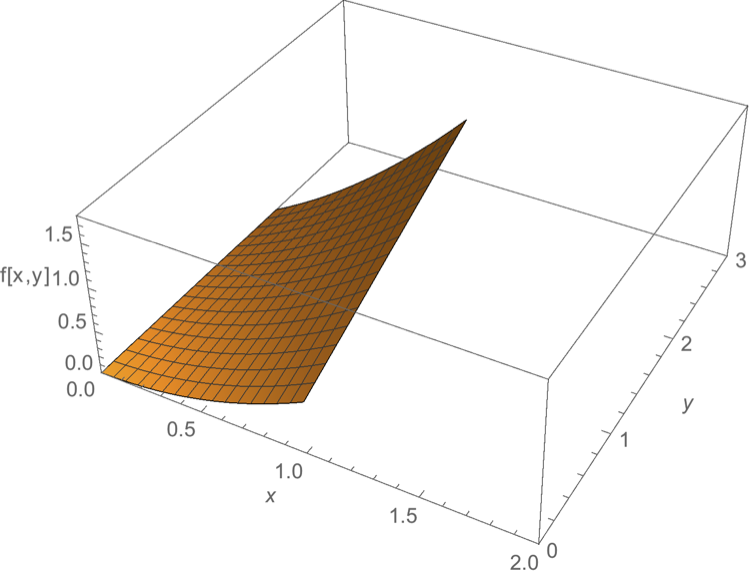
\includegraphics[width=\linewidth]{./images/little_f.png}
\end{image}%
\tcblower
\end{figureptx}%
\textbf{\blocktitlefont Hint}.\quad{}Set up and evaluate a double integral. Here instead of area under a curve, we are looking for the volume under a surface that has been accumulated over the region of interest.%
\end{example}
\begin{theorem}{conditions for a joint probability density.}{}{x:theorem:thm-continuous-th-3-7-cont}%
A bivariate function can serve as a joint probability density for a pair of continuous random variables \(X\) and \(Y\) if and only if its values, \(f(x, y)\), satisfy the conditions%
\begin{enumerate}
\item{}\(f(x, y) \ge 0\)  \(-\infty \lt x, y\lt \infty\);%
\item{}\(\displaystyle\int_{-\infty}^\infty\int_{-\infty}^\infty f(x, y) \,dy\,dx=1\).%
\end{enumerate}
%
\end{theorem}
\begin{definition}{joint distribution function (continuous).}{x:definition:def-joint-density-function-3-7-cont}%
If \(X\) and \(Y\) are continuous random variables, the function given by%
\begin{equation*}
F(x, y) = P(X \le x, Y \le y) = \int_{-\infty}^y\int_{-\infty}^x f(s, t)
\,ds\,dt\text{ for } -\infty \lt x, y \lt \infty
\end{equation*}
where \(f(s,
t)\) is the value of the joint probability density of \(X\) and \(Y\) at \((s, t)\), is called the \terminology{joint density function} or \terminology{joint cumulative density} of \(X\) and \(Y\).%
\end{definition}
\begin{example}{joint CDF.}{x:example:ex-joint-cdf}%
Consider%
\begin{equation*}
f(x) = \begin{cases}\dfrac{3}{5}\Big(x\Big(x+y\Big)\Big),\amp \quad 0 \lt x \lt 1; 0 \lt y \lt 2\\
0,\amp \quad \text{otherwise}\end{cases}
\end{equation*}
and use it to find \(F(x, y) = P(X \lt x, Y \lt y)\).%
\textbf{\blocktitlefont Hint}.\quad{}Set up and evaluate a double integral to an arbitrary point in the plane.%
\textbf{\blocktitlefont Solution}.\quad{}Here instead of area under a curve, we are looking for the volume under a surface that has been accumulated up to the arbitrary point \((x, y)\).%
\begin{equation*}
\begin{aligned}[t]
F(x,y) = 
\begin{cases}
0 \amp \quad x\le 0\text{ or }y\le 0\\
\dfrac{3x^2y^2}{20} + \dfrac{x^3y}{5} \amp \quad 0 \lt x \lt 1, 0 \lt y \lt 2\\
\dfrac{3y^2}{20}+\dfrac{y}{5} \amp \quad  1\le x, 0 \lt y \lt 2\\
\dfrac{12x^2}{20} +\dfrac{6x^3}{15} \amp \quad 0 \lt x \lt 1, 2\le y\\
1 \amp \quad 1\le x, 2\le y
\end{cases}
\end{aligned}
\end{equation*}
Notice that for \(x \ge 1\) and \(0 \lt y \lt 2\), the result depends only on the \(y\)-value, we are no longer accumulating probability in the \(x\)-direction (lower right region in \hyperref[x:figure:fig-ex-joint-cdf]{Figure~{\xreffont\ref{x:figure:fig-ex-joint-cdf}}}).  Reversing the roles of the variables, the is true for the upper left region where \(0 \lt x \lt 1\) and \(y \ge 2\). \begin{figureptx}{Graph of the joint cumulative distribution function.}{x:figure:fig-ex-joint-cdf}{}%
\begin{image}{0.25}{0.5}{0.25}%
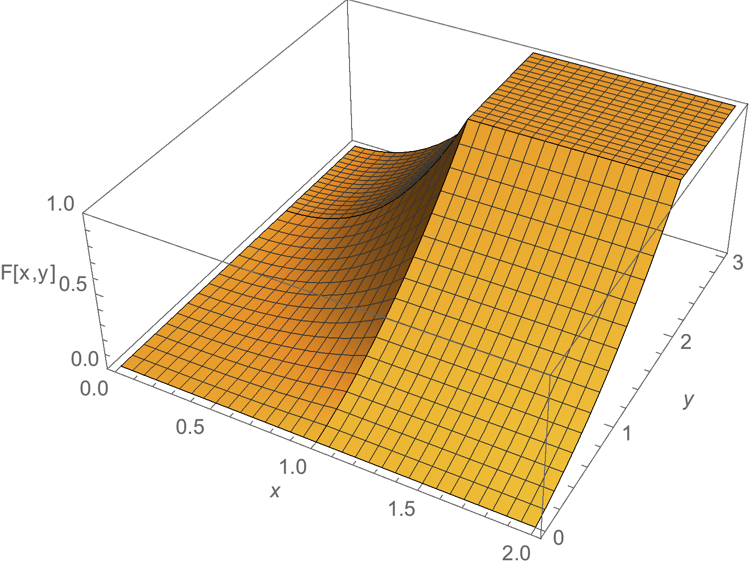
\includegraphics[width=\linewidth]{./images/big_F.png}
\end{image}%
\tcblower
\end{figureptx}%
\end{example}
\begin{remark}{}{x:remark:rmk-jpdf-jcdf}%
Motivated by \(f(x) = \dfrac{dF}{dx}\) we have%
\begin{equation*}
f(x, y) = \dfrac{\partial^2}{\partial x \partial y}\Big(F(x, y)\Big)
\end{equation*}
%
\end{remark}
\begin{definition}{marginal density.}{x:definition:def-marginal-density-3-10-cont}%
If \(X\) and \(Y\) are continuous random variables and \(f(x,
y)\) is the value of their joint probability density at \((x, y)\), the function given by%
\begin{equation*}
g(x) = \int f(x, y)\, dy
\end{equation*}
for each \(x\) within the range of \(X\) is called the \terminology{marginal density} of \(X\). Correspondingly, the function given by%
\begin{equation*}
h(y) = \int f(x, y)\,dx
\end{equation*}
for each \(y\) within the range of \(Y\) is called the \terminology{marginal density} of \(Y\).%
\end{definition}
\begin{inlineexercise}{marginal densities.}{g:exercise:idp140361459998848}%
Calculate the marginal densities of the joint probability distribution used in \hyperref[x:example:ex-joint]{Example~{\xreffont\ref{x:example:ex-joint}}} and \hyperref[x:example:ex-joint-cdf]{Example~{\xreffont\ref{x:example:ex-joint-cdf}}}%
\end{inlineexercise}
\begin{definition}{conditional density.}{x:definition:def-conditional-density-3-10-cont}%
conditional density%
\begin{equation*}
f(x|y) = \dfrac{f(x, y)}{h(y)}, h(y)\ne 0
\end{equation*}
%
\begin{equation*}
w(y|x) = \dfrac{f(x, y)}{g(x)}, g(x)\ne 0
\end{equation*}
%
\end{definition}
\end{subsectionptx}
%
%
\typeout{************************************************}
\typeout{Subsection 5.2.2 Product moments}
\typeout{************************************************}
%
\begin{subsectionptx}{Product moments}{}{Product moments}{}{}{x:subsection:sub-product-moments-cont}
See section 4.6.%
\begin{definition}{product moments about the origin.}{x:definition:def-product-moments-origin-4-7-cont}%
The \terminology{\(\displaystyle r^\text{th}\) and \(\displaystyle
s^\text{th}\) product moment about the origin} of the random variables \(X\) and \(Y\), denoted by \(\displaystyle \mu_{r,s}\), is the expected value of \(\displaystyle X^rY^s\); symbolically%
\begin{equation*}
\mu_{r,s}'=E[X^rY^s] = \int\int x^r y^s\cdot f(x, y)\,dy\,dx
\end{equation*}
\(\displaystyle r = 0,1,2, \dots\) and \(\displaystyle s = 0,1,2,
\dots\) when \(X\) and Y are discrete.%
\end{definition}
Special cases of product moments are \(\displaystyle \mu_{1,0}' =
E[X^1Y^0] = E[X] = \mu_X\) and \(\displaystyle \mu_{0,1}' = E[X^0Y^1]
= E[Y] = \mu_Y\).%
\begin{definition}{product moments about the mean.}{x:definition:def-product-moments-mean-4-8-cont}%
The \terminology{\(\displaystyle r^\text{th}\) and \(\displaystyle
s^\text{th}\) product moment about the mean} of the random variables \(X\) and \(Y\), denoted by \(\displaystyle \mu_{r,s}'\), is the expected value of \(\displaystyle (X-\mu_X)^r(Y-\mu_Y)^s\); symbolically%
\begin{equation*}
\mu_{r,s}=E[(X-\mu_X)^r(Y-\mu_Y)^s] = \int\int (x-\mu_X)^r
(y-\mu_Y)^s\cdot f(x, y)\,dy\,dx
\end{equation*}
\(\displaystyle r = 0,1,2, \dots\) and \(\displaystyle s = 0,1,2, \dots\) when \(X\) and \(Y\) are continuous.%
\end{definition}
Now would be a good time to review \hyperref[x:definition:def-covariance-4-9]{Definition~{\xreffont\ref{x:definition:def-covariance-4-9}}}, \hyperref[x:theorem:thm-4-11]{Theorem~{\xreffont\ref{x:theorem:thm-4-11}}}, \hyperref[x:theorem:thm-4-12]{Theorem~{\xreffont\ref{x:theorem:thm-4-12}}}, \hyperref[x:remark:rmrk-4-12]{Remark~{\xreffont\ref{x:remark:rmrk-4-12}}}, and \hyperref[x:theorem:thm-4-13]{Theorem~{\xreffont\ref{x:theorem:thm-4-13}}} all of which apply here as well.%
\par
Independence means covariance is zero, but covariances of zero does not mean independence.%
\end{subsectionptx}
%
%
\typeout{************************************************}
\typeout{Exercises 5.2.3 Exercises}
\typeout{************************************************}
%
\begin{exercises-subsection}{Exercises}{}{Exercises}{}{}{g:exercises:idp140361460027824}
\begin{divisionexercise}{1}{Problem 4.41.}{}{g:exercise:idp140361460028048}%
If \(X\) and \(Y\) have the joint probability distribution \(f(x, y) = \dfrac{1}{4}\) for \((-3, -5)\),  \((-1, -1)\), \((1, 1)\),  \((3, 5)\), find \(\operatorname{cov}(X, Y)\).%
\end{divisionexercise}%
\begin{divisionexercise}{2}{Problem 4.45.}{}{g:exercise:idp140361460028560}%
If \(X\) and \(Y\) have the joint probability distribution \(f(-1, 0) = 0\),  \(f(-1, 1) = \dfrac{1}{4}\), \(f(0, 0) = \dfrac{1}{6}\), \(f(1, 0) = \dfrac{1}{12}\), \(f(1,
1) = \dfrac{1}{2}\) show that%
\begin{enumerate}[label=(\alph*)]
\item{}\(\operatorname{cov}(X, Y) = 0\);%
\item{}the two random variables are not independent.%
\end{enumerate}
%
\end{divisionexercise}%
\end{exercises-subsection}
%
%
\typeout{************************************************}
\typeout{Subsection 5.2.4 Conditional expectation}
\typeout{************************************************}
%
\begin{subsectionptx}{Conditional expectation}{}{Conditional expectation}{}{}{x:subsection:sub-conditional-expectation}
See section 4.8.%
\begin{definition}{conditional expectation.}{x:definition:def-conditional-expectation-4-10}%
If \(X\) is a discrete random variable and \(\displaystyle f(x|y)\) is the value of the conditional probability distribution of \(X\) given \(\displaystyle Y = y\) at \(X\), the \terminology{conditional expectation} of \(\displaystyle u(X)\) given \(\displaystyle Y = y\) is%
\begin{equation*}
E[u(X)|y] = \int u(x)\cdot f(x|y)\,dx
\end{equation*}
and the \terminology{conditional expectation} of \(\displaystyle v(Y)\) given \(\displaystyle X
= x\) is%
\begin{equation*}
E[v(Y)|x] = \int v(y)\cdot w(y|x)\,dy
\end{equation*}
%
\end{definition}
\begin{definition}{conditional mean.}{x:definition:def-conditional-mean}%
If \(X\) is a discrete random variable and \(\displaystyle f(x|y)\) is the value of the conditional probability distribution of \(X\) given \(\displaystyle Y = y\) at \(X\), the \terminology{conditional mean} of \(\displaystyle u(X) = X\) given \(\displaystyle Y = y\) is%
\begin{equation*}
\mu_{X|y} = E[X|y] = \int x\cdot f(x|y)\,dx
\end{equation*}
and the \terminology{conditional mean} of \(\displaystyle v(Y) = Y\) given \(\displaystyle X = x\) is%
\begin{equation*}
\displaystyle \mu_{Y|x} = E[Y|x] = \int y\cdot w(y|x)\,dy
\end{equation*}
%
\end{definition}
\begin{definition}{conditional variance.}{x:definition:def-conditional-variance}%
If \(X\) is a discrete random variable and \(\displaystyle f(x|y)\) is the value of the conditional probability distribution of \(X\) given \(\displaystyle Y = y\) at \(X\), the \terminology{conditional variance} of \(X\) given \(\displaystyle Y = y\) is%
\begin{equation*}
\sigma^2_{X|y} = E[(X-\mu_{X|y})^2|y] = E[X^2]-\mu^2_{X|y}
\end{equation*}
and the \terminology{conditional expectation} of \(Y\) given \(\displaystyle X = x\) is%
\begin{equation*}
\displaystyle\sigma^2_{Y|x} = E[(Y-\mu_{Y|x})^2|y] =
E[Y^2]-\mu^2_{Y|x}
\end{equation*}
%
\end{definition}
\end{subsectionptx}
\end{sectionptx}
\end{chapterptx}
%
%% A lineskip in table of contents as transition to appendices, backmatter
\addtocontents{toc}{\vspace{\normalbaselineskip}}
%
%
%
\typeout{************************************************}
\typeout{Appendix A Definitions}
\typeout{************************************************}
%
%
\appendix
%
\begin{appendixptx}{Definitions}{}{Definitions}{}{}{x:appendix:appendix-def}
\noindent
\begin{longtable}[l]{ll}
\addtocounter{table}{-1}
\endfirsthead
\endhead
\multicolumn{2}{r}{(Continued on next page)}\\
\endfoot
\endlastfoot
\multicolumn{2}{l}{\null}\\[1.5ex] \multicolumn{2}{l}{\large Section 1.1 Counting}\\[0.5ex]
\hyperref[x:definition:counting]{Definition 1.1.1}& \\
\multicolumn{2}{l}{\null}\\[1.5ex] \multicolumn{2}{l}{\large Section 2.1 Probability}\\[0.5ex]
\hyperref[x:definition:probability]{Definition 2.1.1}& \\
\multicolumn{2}{l}{\null}\\[1.5ex] \multicolumn{2}{l}{\large Section 3.1 Probability distributions}\\[0.5ex]
\hyperref[x:definition:def-probability-distribution-3-2]{Definition 3.1.1}& probability distribution\\
\hyperref[x:definition:def-distribution-function-3-3]{Definition 3.1.3}& distribution function\\
\multicolumn{2}{l}{\null}\\[1.5ex] \multicolumn{2}{l}{\large Section 3.2 Mathematical expectation of discrete random variables}\\[0.5ex]
\hyperref[x:definition:def-expected-value-4-1]{Definition 3.2.1}& expected value\\
\hyperref[x:definition:def-moments-about-origin-4-2]{Definition 3.2.7}& moments about the origin\\
\hyperref[x:definition:def-mean-4-3]{Definition 3.2.8}& mean of a discrete random variable\\
\hyperref[x:definition:def-moments-about-mean-4-4]{Definition 3.2.9}& moments about the mean\\
\hyperref[x:definition:def-mgf-4-6]{Definition 3.2.11}& moment-generating function\\
\multicolumn{2}{l}{\null}\\[1.5ex] \multicolumn{2}{l}{\large Section 3.3 Special probability distributions}\\[0.5ex]
\hyperref[x:definition:def-discrete-unif]{Definition 3.3.1}& discrete uniform distribution\\
\hyperref[x:definition:def-bern]{Definition 3.3.4}& Bernoulli distribution\\
\hyperref[x:definition:def-bin]{Definition 3.3.7}& binomial distribution\\
\hyperref[x:definition:def-neg-bin]{Definition 3.3.19}& negative binomial distribution\\
\hyperref[x:definition:def-geom]{Definition 3.3.24}& geometric distribution\\
\hyperref[x:definition:def-hyper]{Definition 3.3.26}& hypergeometric distribution\\
\hyperref[x:definition:def-poiss]{Definition 3.3.31}& Poisson distribution\\
\multicolumn{2}{l}{\null}\\[1.5ex] \multicolumn{2}{l}{\large Section 4.1 Probability densities}\\[0.5ex]
\hyperref[x:definition:def-continuous-probability-density-3-2]{Definition 4.1.1}& Probability density function\\
\hyperref[x:definition:def-continuous-distribution-function-3-3]{Definition 4.1.9}& \\
\multicolumn{2}{l}{\null}\\[1.5ex] \multicolumn{2}{l}{\large Section 4.2 Expectation of continuous random variables}\\[0.5ex]
\hyperref[x:definition:def-expected-value-4-1-cont]{Definition 4.2.1}& expected value (continuous)\\
\hyperref[x:definition:def-moments-about-origin-4-2-cont]{Definition 4.2.4}& moments about the origin (continuous)\\
\hyperref[x:definition:def-moments-about-mean-4-4-cont]{Definition 4.2.5}& moments about the mean (continuous)\\
\hyperref[x:definition:def-mgf-4-6-cont]{Definition 4.2.8}& moment-generating function (continuous)\\
\multicolumn{2}{l}{\null}\\[1.5ex] \multicolumn{2}{l}{\large Section 4.3 Special probability densities}\\[0.5ex]
\hyperref[x:definition:def-cont-unif]{Definition 4.3.1}& continuous uniform distribution\\
\hyperref[x:definition:def-gamma-func]{Definition 4.3.5}& gamma function\\
\hyperref[x:definition:def-cont-gamma]{Definition 4.3.8}& gamma distribution\\
\hyperref[x:definition:def-cont-exp]{Definition 4.3.15}& exponential distribution\\
\hyperref[x:definition:def-cont-chi]{Definition 4.3.20}& chi-suqare distribution\\
\hyperref[x:definition:def-cont-beta]{Definition 4.3.21}& Beta distribution\\
\hyperref[x:definition:def-cont-normal]{Definition 4.3.24}& Normal distribution\\
\multicolumn{2}{l}{\null}\\[1.5ex] \multicolumn{2}{l}{\large Section 5.1 Multivariate discrete random variables}\\[0.5ex]
\hyperref[x:definition:def-joint-probability-distribution-3-6]{Definition 5.1.1}& joint probability distribution\\
\hyperref[x:definition:def-joint-distribution-function-3-7]{Definition 5.1.3}& joint distribution function\\
\hyperref[x:definition:def-marginal-distribution-3-10]{Definition 5.1.4}& marginal distribution\\
\hyperref[x:definition:def-conditional-distribution-3-10]{Definition 5.1.5}& conditional distribution\\
\hyperref[x:definition:def-product-moments-origin-4-7]{Definition 5.1.8}& product moments about the origin\\
\hyperref[x:definition:def-product-moments-mean-4-8]{Definition 5.1.9}& product moments about the mean\\
\hyperref[x:definition:def-covariance-4-9]{Definition 5.1.10}& covariance\\
\hyperref[x:definition:def-conditional-expectation-4-10]{Definition 5.1.20}& conditional expectation\\
\hyperref[x:definition:def-conditional-mean]{Definition 5.1.21}& conditional mean\\
\hyperref[x:definition:def-conditional-variance]{Definition 5.1.22}& conditional variance\\
\multicolumn{2}{l}{\null}\\[1.5ex] \multicolumn{2}{l}{\large Section 5.2 Multivariate continuous random variables}\\[0.5ex]
\hyperref[x:definition:def-joint-probability-density-3-6-cont]{Definition 5.2.1}& joint probability density\\
\hyperref[x:definition:def-joint-density-function-3-7-cont]{Definition 5.2.5}& joint distribution function (continuous)\\
\hyperref[x:definition:def-marginal-density-3-10-cont]{Definition 5.2.9}& marginal density\\
\hyperref[x:definition:def-conditional-density-3-10-cont]{Definition 5.2.11}& conditional density\\
\hyperref[x:definition:def-product-moments-origin-4-7-cont]{Definition 5.2.12}& product moments about the origin\\
\hyperref[x:definition:def-product-moments-mean-4-8-cont]{Definition 5.2.13}& product moments about the mean\\
\hyperref[x:definition:def-conditional-expectation-4-10]{Definition 5.2.14}& conditional expectation\\
\hyperref[x:definition:def-conditional-mean]{Definition 5.2.15}& conditional mean\\
\hyperref[x:definition:def-conditional-variance]{Definition 5.2.16}& conditional variance\\
\end{longtable}
\end{appendixptx}
%
%
\typeout{************************************************}
\typeout{Appendix B Theorems}
\typeout{************************************************}
%
\begin{appendixptx}{Theorems}{}{Theorems}{}{}{x:appendix:appendix-thm}
\noindent
\begin{longtable}[l]{ll}
\addtocounter{table}{-1}
\endfirsthead
\endhead
\multicolumn{2}{r}{(Continued on next page)}\\
\endfoot
\endlastfoot
\multicolumn{2}{l}{\null}\\[1.5ex] \multicolumn{2}{l}{\large Section 3.1 Probability distributions}\\[0.5ex]
\hyperref[x:theorem:thm-conditions-3-1]{Theorem 3.1.2}& conditions for probability distribution\\
\hyperref[x:theorem:thm-3-2]{Theorem 3.1.4}& properties of a distribution function\\
\multicolumn{2}{l}{\null}\\[1.5ex] \multicolumn{2}{l}{\large Section 3.2 Mathematical expectation of discrete random variables}\\[0.5ex]
\hyperref[x:theorem:thm-expected-value-function-random-variable-4-1]{Theorem 3.2.3}& expected value of a function of a random variable\\
\hyperref[x:theorem:thm-4-2]{Theorem 3.2.4}& expectation of a linear function\\
\hyperref[x:theorem:thm-4-9]{Theorem 3.2.14}& moments via differentiation\\
\hyperref[x:theorem:thm-4-10]{Theorem 3.2.16}& moment-generating function of functions of a random variable\\
\multicolumn{2}{l}{\null}\\[1.5ex] \multicolumn{2}{l}{\large Section 3.3 Special probability distributions}\\[0.5ex]
\hyperref[x:theorem:thm-bin-param]{Theorem 3.3.13}& reparameterizing a binomial\\
\hyperref[x:theorem:thm-bin-mean-var]{Theorem 3.3.15}& Mean and variance of binomial distribution\\
\hyperref[x:theorem:thm-bin-successes]{Theorem 3.3.16}& Proportion of binomial successes\\
\hyperref[x:theorem:thm-bin-negbin]{Theorem 3.3.20}& negative binomial probability as a binomial probability\\
\hyperref[g:theorem:idp140361459544288]{Theorem 3.3.22}& Mean and variance of the negative binomial distribution\\
\hyperref[g:theorem:idp140361459555536]{Theorem 3.3.25}& Mean and variance of the geometric distribution\\
\hyperref[g:theorem:idp140361459569280]{Theorem 3.3.27}& Mean and variance of the hypergeometric distribution\\
\hyperref[g:theorem:idp140361459590528]{Theorem 3.3.32}& Mean, variance, and MGF of the Poisson distribution\\
\multicolumn{2}{l}{\null}\\[1.5ex] \multicolumn{2}{l}{\large Section 4.1 Probability densities}\\[0.5ex]
\hyperref[x:theorem:thm-continuous-point]{Theorem 4.1.4}& probability density at a point\\
\hyperref[x:theorem:thm-continuous-conditions-3-1]{Theorem 4.1.5}& conditions for probability density\\
\hyperref[x:theorem:thm-continuous-th-3-2]{Theorem 4.1.12}& distribution function (continuous)\\
\hyperref[x:theorem:thm-pdf-cdf]{Theorem 4.1.13}& density from distribution function\\
\multicolumn{2}{l}{\null}\\[1.5ex] \multicolumn{2}{l}{\large Section 4.2 Expectation of continuous random variables}\\[0.5ex]
\hyperref[x:theorem:thm-expected-value-function-random-variable-4-1-cont]{Theorem 4.2.3}& expected value of a function of a random variable (continuous)\\
\hyperref[x:theorem:thm-chebyshev]{Theorem 4.2.7}& Chebyshev's Theorem\\
\multicolumn{2}{l}{\null}\\[1.5ex] \multicolumn{2}{l}{\large Section 4.3 Special probability densities}\\[0.5ex]
\hyperref[x:theorem:thm-cont-unif-mean]{Theorem 4.3.3}& mean and variance of continuous uniform\\
\hyperref[x:theorem:thm-cont-gamma-moments]{Theorem 4.3.10}& moments about the origin of the gamma\\
\hyperref[x:theorem:thm-cont-gamma-mean]{Theorem 4.3.11}& mean and variance of gamma\\
\hyperref[x:theorem:thm-cont-gamma-mgf]{Theorem 4.3.12}& moment-generating function of the gamma\\
\hyperref[x:theorem:thm-cont-normal-mean]{Theorem 4.3.25}& mean and variance of normal\\
\hyperref[x:theorem:thm-cont-normal-mgf]{Theorem 4.3.26}& moment-generating function of the normal\\
\hyperref[x:theorem:thm-cont-std-normal]{Theorem 4.3.31}& transforming to standard normal\\
\hyperref[x:theorem:thm-cont-normal-binom]{Theorem 4.3.38}& normal approximation to the binomial\\
\multicolumn{2}{l}{\null}\\[1.5ex] \multicolumn{2}{l}{\large Section 5.1 Multivariate discrete random variables}\\[0.5ex]
\hyperref[x:theorem:thm-3-7]{Theorem 5.1.2}& conditions for a joint probability distribution\\
\hyperref[x:theorem:thm-expected-value-joint-random-variables-4-4]{Theorem 5.1.6}& expected value of joint random variables\\
\hyperref[x:theorem:thm-4-5]{Theorem 5.1.7}& expected value of a linear combination of random variables\\
\hyperref[x:theorem:thm-4-11]{Theorem 5.1.11}& covariance from moments about the origin\\
\hyperref[x:theorem:thm-4-12]{Theorem 5.1.12}& independence and covariance\\
\hyperref[x:theorem:thm-4-13]{Theorem 5.1.14}& product moments of independent random variables\\
\hyperref[x:theorem:thm-4-14]{Theorem 5.1.15}& variance\\
\hyperref[x:theorem:thm-4-15]{Theorem 5.1.18}& covariance of two linear combinations\\
\multicolumn{2}{l}{\null}\\[1.5ex] \multicolumn{2}{l}{\large Section 5.2 Multivariate continuous random variables}\\[0.5ex]
\hyperref[x:theorem:thm-continuous-th-3-7-cont]{Theorem 5.2.4}& conditions for a joint probability density\\
\end{longtable}
\end{appendixptx}
%
%
\typeout{************************************************}
\typeout{Appendix C Examples}
\typeout{************************************************}
%
\begin{appendixptx}{Examples}{}{Examples}{}{}{x:appendix:appendix-ex}
\noindent
\begin{longtable}[l]{ll}
\addtocounter{table}{-1}
\endfirsthead
\endhead
\multicolumn{2}{r}{(Continued on next page)}\\
\endfoot
\endlastfoot
\multicolumn{2}{l}{\null}\\[1.5ex] \multicolumn{2}{l}{\large Section 3.1 Probability distributions}\\[0.5ex]
\hyperref[x:example:ex-disc-pmf]{Example 3.1.5}& Verifying a simple probability mass function\\
\hyperref[x:example:ex-disc-pmf-to-cdf]{Example 3.1.8}& CDF of a simple probability mass function\\
\multicolumn{2}{l}{\null}\\[1.5ex] \multicolumn{2}{l}{\large Section 3.2 Mathematical expectation of discrete random variables}\\[0.5ex]
\hyperref[x:example:ex-disc-pmf-mean]{Example 3.2.2}& expected value of a random variable\\
\hyperref[x:example:ex-disc-pmf-variance]{Example 3.2.10}& variance of a random variable\\
\hyperref[x:example:ex-maclaurin]{Example 3.2.12}& moment-generating function via Taylor series\\
\hyperref[x:example:ex-three-coins-mgf]{Example 3.2.13}& moment-generating function for three coins\\
\hyperref[x:example:ex-three-coins-mgf2]{Example 3.2.15}& moment-generating function for three cards, via differentiation\\
\multicolumn{2}{l}{\null}\\[1.5ex] \multicolumn{2}{l}{\large Section 3.3 Special probability distributions}\\[0.5ex]
\hyperref[x:example:ex-disc-unif-mean]{Example 3.3.2}& mean of a discrete uniform distribution\\
\hyperref[x:example:ex-disc-unif-simple]{Example 3.3.3}& simple discrete uniform distribution\\
\hyperref[x:example:ex-bern-mean-var]{Example 3.3.5}& mean and variance of a Bernoulli distribution\\
\hyperref[x:example:ex-bern-mgf]{Example 3.3.6}& moment-generating function of a Bernoulli distribution\\
\hyperref[x:example:ex-bin-basketball-dumb]{Example 3.3.9}& Basketball free throws\\
\hyperref[x:example:ex-bin-bball]{Example 3.3.11}& Free throws\\
\hyperref[x:example:ex-bin-coins]{Example 3.3.12}& Binomial coin flips\\
\hyperref[x:example:ex-bin-bball2]{Example 3.3.14}& Free throws - revisited\\
\hyperref[x:example:ex-bin-mgf]{Example 3.3.18}& moment-generating function of a binomial distribution\\
\hyperref[x:example:ex-negbin-mgf]{Example 3.3.23}& moment generating function of the negative binomial distribution\\
\hyperref[x:example:ex-hyper]{Example 3.3.29}& hypergeometric distribution for truck inspections\\
\multicolumn{2}{l}{\null}\\[1.5ex] \multicolumn{2}{l}{\large Section 4.1 Probability densities}\\[0.5ex]
\hyperref[x:example:ex-exponential]{Example 4.1.6}& specifying an exponential probability density\\
\hyperref[x:example:ex-exponential2]{Example 4.1.7}& using exponential probability density\\
\hyperref[x:example:ex-hat]{Example 4.1.8}& a hat-shaped probability density\\
\hyperref[x:example:ex-hat-cdf]{Example 4.1.11}& cumulative distribution for a hat-shaped probability density\\
\hyperref[x:example:ex-F-to-f]{Example 4.1.15}& a ramp-shaped cumulative distribution\\
\multicolumn{2}{l}{\null}\\[1.5ex] \multicolumn{2}{l}{\large Section 4.2 Expectation of continuous random variables}\\[0.5ex]
\hyperref[x:example:ex-cont-exp]{Example 4.2.2}& expected value (continuous)\\
\hyperref[x:example:ex-poly]{Example 4.2.6}& \(8^{\text{th}}\)-order polynomial density\\
\hyperref[x:example:ex-exp-MGF]{Example 4.2.9}& moment-generating function by definition\\
\hyperref[x:example:ex-exp-mgf-by-diff]{Example 4.2.10}& moments of an exponential by differentiation\\
\multicolumn{2}{l}{\null}\\[1.5ex] \multicolumn{2}{l}{\large Section 4.3 Special probability densities}\\[0.5ex]
\hyperref[x:example:ex-std-norm-probs]{Example 4.3.32}& probabilities from the standard normal\\
\hyperref[x:example:ex-std-norm-probs2]{Example 4.3.37}& probabilities from the standard normal\\
\multicolumn{2}{l}{\null}\\[1.5ex] \multicolumn{2}{l}{\large Section 5.1 Multivariate discrete random variables}\\[0.5ex]
\hyperref[x:example:ex-var-covar]{Example 5.1.17}& covariances of linear combinations\\
\multicolumn{2}{l}{\null}\\[1.5ex] \multicolumn{2}{l}{\large Section 5.2 Multivariate continuous random variables}\\[0.5ex]
\hyperref[x:example:ex-joint]{Example 5.2.2}& jointly-distributed random variables\\
\hyperref[x:example:ex-joint-cdf]{Example 5.2.6}& joint CDF\\
\end{longtable}
\end{appendixptx}
%
%
\typeout{************************************************}
\typeout{Appendix D GNU Free Documentation License}
\typeout{************************************************}
%
\begin{appendixptx}{GNU Free Documentation License}{}{GNU Free Documentation License}{}{}{x:appendix:appendix-gfdl}
Version 1.3, 3 November 2008%
\par
Copyright \textcopyright{} 2000, 2001, 2002, 2007, 2008 Free Software Foundation, Inc. \textless{}\url{http://www.fsf.org/}\textgreater{}%
\par
Everyone is permitted to copy and distribute verbatim copies of this license document, but changing it is not allowed.%
\begin{paragraphs}{0. PREAMBLE.}{x:paragraphs:gfdl-section0}%
The purpose of this License is to make a manual, textbook, or other functional and useful document ``free'' in the sense of freedom: to assure everyone the effective freedom to copy and redistribute it, with or without modifying it, either commercially or noncommercially. Secondarily, this License preserves for the author and publisher a way to get credit for their work, while not being considered responsible for modifications made by others.%
\par
This License is a kind of ``copyleft'', which means that derivative works of the document must themselves be free in the same sense. It complements the GNU General Public License, which is a copyleft license designed for free software.%
\par
We have designed this License in order to use it for manuals for free software, because free software needs free documentation: a free program should come with manuals providing the same freedoms that the software does. But this License is not limited to software manuals; it can be used for any textual work, regardless of subject matter or whether it is published as a printed book. We recommend this License principally for works whose purpose is instruction or reference.%
\end{paragraphs}%
\begin{paragraphs}{1. APPLICABILITY AND DEFINITIONS.}{x:paragraphs:gfdl-section1}%
This License applies to any manual or other work, in any medium, that contains a notice placed by the copyright holder saying it can be distributed under the terms of this License. Such a notice grants a world-wide, royalty-free license, unlimited in duration, to use that work under the conditions stated herein. The ``Document'', below, refers to any such manual or work. Any member of the public is a licensee, and is addressed as ``you''. You accept the license if you copy, modify or distribute the work in a way requiring permission under copyright law.%
\par
A ``Modified Version'' of the Document means any work containing the Document or a portion of it, either copied verbatim, or with modifications and\slash{}or translated into another language.%
\par
A ``Secondary Section'' is a named appendix or a front-matter section of the Document that deals exclusively with the relationship of the publishers or authors of the Document to the Document's overall subject (or to related matters) and contains nothing that could fall directly within that overall subject. (Thus, if the Document is in part a textbook of mathematics, a Secondary Section may not explain any mathematics.) The relationship could be a matter of historical connection with the subject or with related matters, or of legal, commercial, philosophical, ethical or political position regarding them.%
\par
The ``Invariant Sections'' are certain Secondary Sections whose titles are designated, as being those of Invariant Sections, in the notice that says that the Document is released under this License. If a section does not fit the above definition of Secondary then it is not allowed to be designated as Invariant. The Document may contain zero Invariant Sections. If the Document does not identify any Invariant Sections then there are none.%
\par
The ``Cover Texts'' are certain short passages of text that are listed, as Front-Cover Texts or Back-Cover Texts, in the notice that says that the Document is released under this License. A Front-Cover Text may be at most 5 words, and a Back-Cover Text may be at most 25 words.%
\par
A ``Transparent'' copy of the Document means a machine-readable copy, represented in a format whose specification is available to the general public, that is suitable for revising the document straightforwardly with generic text editors or (for images composed of pixels) generic paint programs or (for drawings) some widely available drawing editor, and that is suitable for input to text formatters or for automatic translation to a variety of formats suitable for input to text formatters. A copy made in an otherwise Transparent file format whose markup, or absence of markup, has been arranged to thwart or discourage subsequent modification by readers is not Transparent. An image format is not Transparent if used for any substantial amount of text. A copy that is not ``Transparent'' is called ``Opaque''.%
\par
Examples of suitable formats for Transparent copies include plain ASCII without markup, Texinfo input format, LaTeX input format, SGML or XML using a publicly available DTD, and standard-conforming simple HTML, PostScript or PDF designed for human modification. Examples of transparent image formats include PNG, XCF and JPG. Opaque formats include proprietary formats that can be read and edited only by proprietary word processors, SGML or XML for which the DTD and\slash{}or processing tools are not generally available, and the machine-generated HTML, PostScript or PDF produced by some word processors for output purposes only.%
\par
The ``Title Page'' means, for a printed book, the title page itself, plus such following pages as are needed to hold, legibly, the material this License requires to appear in the title page. For works in formats which do not have any title page as such, ``Title Page'' means the text near the most prominent appearance of the work's title, preceding the beginning of the body of the text.%
\par
The ``publisher'' means any person or entity that distributes copies of the Document to the public.%
\par
A section ``Entitled XYZ'' means a named subunit of the Document whose title either is precisely XYZ or contains XYZ in parentheses following text that translates XYZ in another language. (Here XYZ stands for a specific section name mentioned below, such as ``Acknowledgements'', ``Dedications'', ``Endorsements'', or ``History''.) To ``Preserve the Title'' of such a section when you modify the Document means that it remains a section ``Entitled XYZ'' according to this definition.%
\par
The Document may include Warranty Disclaimers next to the notice which states that this License applies to the Document. These Warranty Disclaimers are considered to be included by reference in this License, but only as regards disclaiming warranties: any other implication that these Warranty Disclaimers may have is void and has no effect on the meaning of this License.%
\end{paragraphs}%
\begin{paragraphs}{2. VERBATIM COPYING.}{x:paragraphs:gfdl-section2}%
You may copy and distribute the Document in any medium, either commercially or noncommercially, provided that this License, the copyright notices, and the license notice saying this License applies to the Document are reproduced in all copies, and that you add no other conditions whatsoever to those of this License. You may not use technical measures to obstruct or control the reading or further copying of the copies you make or distribute. However, you may accept compensation in exchange for copies. If you distribute a large enough number of copies you must also follow the conditions in section 3.%
\par
You may also lend copies, under the same conditions stated above, and you may publicly display copies.%
\end{paragraphs}%
\begin{paragraphs}{3. COPYING IN QUANTITY.}{x:paragraphs:gfdl-section3}%
If you publish printed copies (or copies in media that commonly have printed covers) of the Document, numbering more than 100, and the Document's license notice requires Cover Texts, you must enclose the copies in covers that carry, clearly and legibly, all these Cover Texts: Front-Cover Texts on the front cover, and Back-Cover Texts on the back cover. Both covers must also clearly and legibly identify you as the publisher of these copies. The front cover must present the full title with all words of the title equally prominent and visible. You may add other material on the covers in addition. Copying with changes limited to the covers, as long as they preserve the title of the Document and satisfy these conditions, can be treated as verbatim copying in other respects.%
\par
If the required texts for either cover are too voluminous to fit legibly, you should put the first ones listed (as many as fit reasonably) on the actual cover, and continue the rest onto adjacent pages.%
\par
If you publish or distribute Opaque copies of the Document numbering more than 100, you must either include a machine-readable Transparent copy along with each Opaque copy, or state in or with each Opaque copy a computer-network location from which the general network-using public has access to download using public-standard network protocols a complete Transparent copy of the Document, free of added material. If you use the latter option, you must take reasonably prudent steps, when you begin distribution of Opaque copies in quantity, to ensure that this Transparent copy will remain thus accessible at the stated location until at least one year after the last time you distribute an Opaque copy (directly or through your agents or retailers) of that edition to the public.%
\par
It is requested, but not required, that you contact the authors of the Document well before redistributing any large number of copies, to give them a chance to provide you with an updated version of the Document.%
\end{paragraphs}%
\begin{paragraphs}{4. MODIFICATIONS.}{x:paragraphs:gfdl-section4}%
You may copy and distribute a Modified Version of the Document under the conditions of sections 2 and 3 above, provided that you release the Modified Version under precisely this License, with the Modified Version filling the role of the Document, thus licensing distribution and modification of the Modified Version to whoever possesses a copy of it. In addition, you must do these things in the Modified Version:%
\begin{enumerate}[label=\Alph*.]
\item{}Use in the Title Page (and on the covers, if any) a title distinct from that of the Document, and from those of previous versions (which should, if there were any, be listed in the History section of the Document). You may use the same title as a previous version if the original publisher of that version gives permission.%
\item{}List on the Title Page, as authors, one or more persons or entities responsible for authorship of the modifications in the Modified Version, together with at least five of the principal authors of the Document (all of its principal authors, if it has fewer than five), unless they release you from this requirement.%
\item{}State on the Title page the name of the publisher of the Modified Version, as the publisher.%
\item{}Preserve all the copyright notices of the Document.%
\item{}Add an appropriate copyright notice for your modifications adjacent to the other copyright notices.%
\item{}Include, immediately after the copyright notices, a license notice giving the public permission to use the Modified Version under the terms of this License, in the form shown in the Addendum below.%
\item{}Preserve in that license notice the full lists of Invariant Sections and required Cover Texts given in the Document's license notice.%
\item{}Include an unaltered copy of this License.%
\item{}Preserve the section Entitled ``History'', Preserve its Title, and add to it an item stating at least the title, year, new authors, and publisher of the Modified Version as given on the Title Page. If there is no section Entitled ``History'' in the Document, create one stating the title, year, authors, and publisher of the Document as given on its Title Page, then add an item describing the Modified Version as stated in the previous sentence.%
\item{}Preserve the network location, if any, given in the Document for public access to a Transparent copy of the Document, and likewise the network locations given in the Document for previous versions it was based on.  These may be placed in the ``History'' section. You may omit a network location for a work that was published at least four years before the Document itself, or if the original publisher of the version it refers to gives permission.%
\item{}For any section Entitled ``Acknowledgements'' or ``Dedications'', Preserve the Title of the section, and preserve in the section all the substance and tone of each of the contributor acknowledgements and\slash{}or dedications given therein.%
\item{}Preserve all the Invariant Sections of the Document, unaltered in their text and in their titles. Section numbers or the equivalent are not considered part of the section titles.%
\item{}Delete any section Entitled ``Endorsements''. Such a section may not be included in the Modified Version.%
\item{}Do not retitle any existing section to be Entitled ``Endorsements'' or to conflict in title with any Invariant Section.%
\item{}Preserve any Warranty Disclaimers.%
\end{enumerate}
%
\par
If the Modified Version includes new front-matter sections or appendices that qualify as Secondary Sections and contain no material copied from the Document, you may at your option designate some or all of these sections as invariant. To do this, add their titles to the list of Invariant Sections in the Modified Version's license notice. These titles must be distinct from any other section titles.%
\par
You may add a section Entitled ``Endorsements'', provided it contains nothing but endorsements of your Modified Version by various parties \textemdash{} for example, statements of peer review or that the text has been approved by an organization as the authoritative definition of a standard.%
\par
You may add a passage of up to five words as a Front-Cover Text, and a passage of up to 25 words as a Back-Cover Text, to the end of the list of Cover Texts in the Modified Version. Only one passage of Front-Cover Text and one of Back-Cover Text may be added by (or through arrangements made by) any one entity. If the Document already includes a cover text for the same cover, previously added by you or by arrangement made by the same entity you are acting on behalf of, you may not add another; but you may replace the old one, on explicit permission from the previous publisher that added the old one.%
\par
The author(s) and publisher(s) of the Document do not by this License give permission to use their names for publicity for or to assert or imply endorsement of any Modified Version.%
\end{paragraphs}%
\begin{paragraphs}{5. COMBINING DOCUMENTS.}{x:paragraphs:gfdl-section5}%
You may combine the Document with other documents released under this License, under the terms defined in section 4 above for modified versions, provided that you include in the combination all of the Invariant Sections of all of the original documents, unmodified, and list them all as Invariant Sections of your combined work in its license notice, and that you preserve all their Warranty Disclaimers.%
\par
The combined work need only contain one copy of this License, and multiple identical Invariant Sections may be replaced with a single copy. If there are multiple Invariant Sections with the same name but different contents, make the title of each such section unique by adding at the end of it, in parentheses, the name of the original author or publisher of that section if known, or else a unique number. Make the same adjustment to the section titles in the list of Invariant Sections in the license notice of the combined work.%
\par
In the combination, you must combine any sections Entitled ``History'' in the various original documents, forming one section Entitled ``History''; likewise combine any sections Entitled ``Acknowledgements'', and any sections Entitled ``Dedications''. You must delete all sections Entitled ``Endorsements''.%
\end{paragraphs}%
\begin{paragraphs}{6. COLLECTIONS OF DOCUMENTS.}{x:paragraphs:gfdl-section6}%
You may make a collection consisting of the Document and other documents released under this License, and replace the individual copies of this License in the various documents with a single copy that is included in the collection, provided that you follow the rules of this License for verbatim copying of each of the documents in all other respects.%
\par
You may extract a single document from such a collection, and distribute it individually under this License, provided you insert a copy of this License into the extracted document, and follow this License in all other respects regarding verbatim copying of that document.%
\end{paragraphs}%
\begin{paragraphs}{7. AGGREGATION WITH INDEPENDENT WORKS.}{x:paragraphs:gfdl-section7}%
A compilation of the Document or its derivatives with other separate and independent documents or works, in or on a volume of a storage or distribution medium, is called an ``aggregate'' if the copyright resulting from the compilation is not used to limit the legal rights of the compilation's users beyond what the individual works permit. When the Document is included in an aggregate, this License does not apply to the other works in the aggregate which are not themselves derivative works of the Document.%
\par
If the Cover Text requirement of section 3 is applicable to these copies of the Document, then if the Document is less than one half of the entire aggregate, the Document's Cover Texts may be placed on covers that bracket the Document within the aggregate, or the electronic equivalent of covers if the Document is in electronic form. Otherwise they must appear on printed covers that bracket the whole aggregate.%
\end{paragraphs}%
\begin{paragraphs}{8. TRANSLATION.}{x:paragraphs:gfdl-section8}%
Translation is considered a kind of modification, so you may distribute translations of the Document under the terms of section 4. Replacing Invariant Sections with translations requires special permission from their copyright holders, but you may include translations of some or all Invariant Sections in addition to the original versions of these Invariant Sections. You may include a translation of this License, and all the license notices in the Document, and any Warranty Disclaimers, provided that you also include the original English version of this License and the original versions of those notices and disclaimers. In case of a disagreement between the translation and the original version of this License or a notice or disclaimer, the original version will prevail.%
\par
If a section in the Document is Entitled ``Acknowledgements'', ``Dedications'', or ``History'', the requirement (section 4) to Preserve its Title (section 1) will typically require changing the actual title.%
\end{paragraphs}%
\begin{paragraphs}{9. TERMINATION.}{x:paragraphs:gfdl-section9}%
You may not copy, modify, sublicense, or distribute the Document except as expressly provided under this License. Any attempt otherwise to copy, modify, sublicense, or distribute it is void, and will automatically terminate your rights under this License.%
\par
However, if you cease all violation of this License, then your license from a particular copyright holder is reinstated (a) provisionally, unless and until the copyright holder explicitly and finally terminates your license, and (b) permanently, if the copyright holder fails to notify you of the violation by some reasonable means prior to 60 days after the cessation.%
\par
Moreover, your license from a particular copyright holder is reinstated permanently if the copyright holder notifies you of the violation by some reasonable means, this is the first time you have received notice of violation of this License (for any work) from that copyright holder, and you cure the violation prior to 30 days after your receipt of the notice.%
\par
Termination of your rights under this section does not terminate the licenses of parties who have received copies or rights from you under this License. If your rights have been terminated and not permanently reinstated, receipt of a copy of some or all of the same material does not give you any rights to use it.%
\end{paragraphs}%
\begin{paragraphs}{10. FUTURE REVISIONS OF THIS LICENSE.}{x:paragraphs:gfdl-section10}%
The Free Software Foundation may publish new, revised versions of the GNU Free Documentation License from time to time. Such new versions will be similar in spirit to the present version, but may differ in detail to address new problems or concerns. See \url{http://www.gnu.org/copyleft/}.%
\par
Each version of the License is given a distinguishing version number. If the Document specifies that a particular numbered version of this License ``or any later version'' applies to it, you have the option of following the terms and conditions either of that specified version or of any later version that has been published (not as a draft) by the Free Software Foundation. If the Document does not specify a version number of this License, you may choose any version ever published (not as a draft) by the Free Software Foundation. If the Document specifies that a proxy can decide which future versions of this License can be used, that proxy's public statement of acceptance of a version permanently authorizes you to choose that version for the Document.%
\end{paragraphs}%
\begin{paragraphs}{11. RELICENSING.}{x:paragraphs:gfdl-section11}%
``Massive Multiauthor Collaboration Site'' (or ``MMC Site'') means any World Wide Web server that publishes copyrightable works and also provides prominent facilities for anybody to edit those works. A public wiki that anybody can edit is an example of such a server. A ``Massive Multiauthor Collaboration'' (or ``MMC'') contained in the site means any set of copyrightable works thus published on the MMC site.%
\par
``CC-BY-SA'' means the Creative Commons Attribution-Share Alike 3.0 license published by Creative Commons Corporation, a not-for-profit corporation with a principal place of business in San Francisco, California, as well as future copyleft versions of that license published by that same organization.%
\par
``Incorporate'' means to publish or republish a Document, in whole or in part, as part of another Document.%
\par
An MMC is ``eligible for relicensing'' if it is licensed under this License, and if all works that were first published under this License somewhere other than this MMC, and subsequently incorporated in whole or in part into the MMC, (1) had no cover texts or invariant sections, and (2) were thus incorporated prior to November 1, 2008.%
\par
The operator of an MMC Site may republish an MMC contained in the site under CC-BY-SA on the same site at any time before August 1, 2009, provided the MMC is eligible for relicensing.%
\end{paragraphs}%
\begin{paragraphs}{ADDENDUM: How to use this License for your documents.}{x:paragraphs:gfdl-addendum}%
To use this License in a document you have written, include a copy of the License in the document and put the following copyright and license notices just after the title page:%
\begin{preformatted}
Copyright (C)  YEAR  YOUR NAME. Permission is granted to
       copy, distribute and/or modify this document under the terms of
       the GNU Free Documentation License, Version 1.3 or any later
       version published by the Free Software Foundation; with no
       Invariant Sections, no Front-Cover Texts, and no Back-Cover
       Texts. A copy of the license is included in the section entitled
       ``GNU Free Documentation License''.
\end{preformatted}
If you have Invariant Sections, Front-Cover Texts and Back-Cover Texts, replace the ``with\textellipsis{} Texts.'' line with this:%
\begin{preformatted}
with the Invariant Sections being LIST THEIR TITLES, with
       the Front-Cover Texts being LIST, and with the Back-Cover Texts
       being LIST.
\end{preformatted}
If you have Invariant Sections without Cover Texts, or some other combination of the three, merge those two alternatives to suit the situation.%
\par
If your document contains nontrivial examples of program code, we recommend releasing these examples in parallel under your choice of free software license, such as the GNU General Public License, to permit their use in free software.%
\end{paragraphs}%
\end{appendixptx}
%
\backmatter
%
%
%% The index is here, setup is all in preamble
%% Index locators are cross-references, so same font here
{\xreffont\printindex}
%
\cleardoublepage
\pagestyle{empty}
\vspace*{\stretch{1}}
\begin{backcolophon}{x:colophon:back-colophon}%
This book was authored in MathBook XML.%
\end{backcolophon}%
\vspace*{\stretch{2}}
%% Back cover image, not numbered
\cleardoublepage%
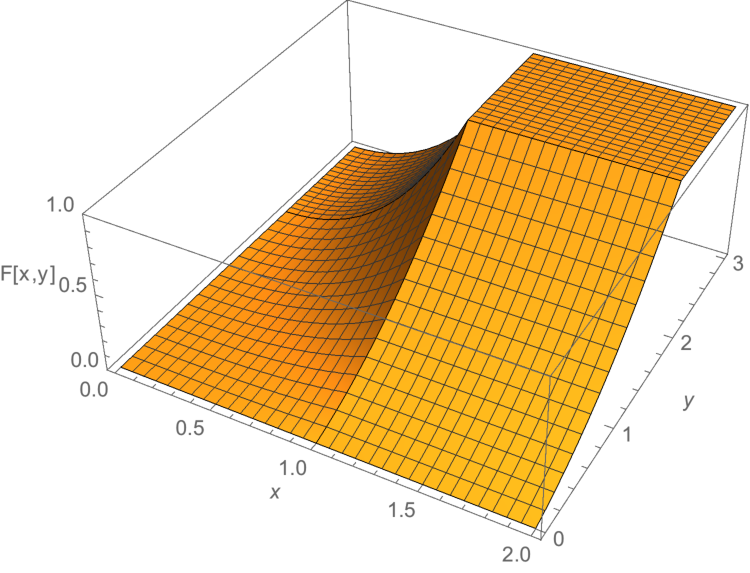
\includepdf[noautoscale=false]{images/cover.pdf}%
\end{document}